\documentclass[a4paper]{report}
\usepackage[utf8]{inputenc}
\usepackage[dvipsnames]{xcolor}
\usepackage{url}
\usepackage{listings}
\usepackage[colorlinks=true,citecolor=blue]{hyperref}
\usepackage{amsmath,amsfonts,amssymb}
\usepackage[margin=2cm]{geometry}
\usepackage{titlesec}
\usepackage{booktabs} %python only so may be removed on update
\usepackage{graphicx}
% \usepackage{lmodern} %to remove `OT1/cmss/m/n' in size <36> not available” warning
% \usepackage[T1]{fontenc}
\usepackage{natbib}
\bibliographystyle{unsrtnat}
\usepackage{pmboxdraw}

% see https://www.overleaf.com/learn/latex/Glossaries
% make glossaries must be written before the first glossary entry
\usepackage[utf8]{inputenc}
\usepackage[acronym, toc]{glossaries}

\newcommand{\publisher}[0]{Geoscience Australia and Frontier-SI}
\newcommand{\authors}[0]{Sebastien Allgeyer, Rupert Brown, John Donovan,
Ken Harima, Aaron Hammond, Lavanya Kumarappan, Tao Li, Ronald Maj,
Bogdan Matviichuk, Simon McClusky, Michael Moore, Thomas Papanikolaou,
Tzupang Tseng, Umma Zannat}




% updating section formatting
\titleformat{\section}
  {\normalfont\fontsize{12}{15}\bfseries}{\thesection}{1em}{}
\titleformat{\subsection}
  {\normalfont\fontsize{10}{10}\bfseries}{\thesubsection}{1em}{}
\titleformat{\chapter}[display]
  {\normalfont\bfseries}{}{0pt}{\Large}

% simple environment to prevent hyphenation 
\newenvironment{nohyphens}{%
  \hyphenpenalty=10000
  \exhyphenpenalty=10000
  \sloppy % Makes TeX obey margins by stretching inter word spaces
}{\par}

% code coloring here
\definecolor{codegreen}{rgb}{0,0.6,0}
\definecolor{codegray}{rgb}{0.5,0.5,0.5}
\definecolor{codepurple}{rgb}{0.58,0,0.82}
\definecolor{backcolour}{rgb}{0.95,0.95,0.92}

\lstdefinestyle{mystyle}
{
	backgroundcolor=\color{backcolour},   
	commentstyle=\color{codegreen},
	keywordstyle=\color{magenta},
	numberstyle=\tiny\color{codegray},
	stringstyle=\color{codepurple},
	basicstyle=\ttfamily\footnotesize,
	breakatwhitespace=false,         
	breaklines=true,                 
	captionpos=b,                    
	keepspaces=true,                 
	numbers=left,                    
	numbersep=5pt,                  
	showspaces=false,                
	showstringspaces=false,
	showtabs=false,                  
	tabsize=4,
}
\lstset{style=mystyle}

% yaml styling below
\newcommand\YAMLcolonstyle{\color{red}\mdseries}
\newcommand\YAMLkeystyle{\color{black}\bfseries}
\newcommand\YAMLvaluestyle{\color{blue}\mdseries}

\makeatletter
% here is a macro expanding to the name of the language
% (handy if you decide to change it further down the road)
\newcommand\language@yaml{yaml}

\expandafter\expandafter\expandafter\lstdefinelanguage
\expandafter{\language@yaml}
{
	keywords={true,false,null,y,n},
	keywordstyle=\color{darkgray}\bfseries,
	basicstyle=\YAMLkeystyle,                                 % assuming a key comes first
	sensitive=false,
	comment=[l]{\#},
	morecomment=[s]{/*}{*/},
	commentstyle=\color{purple},
	stringstyle=\YAMLvaluestyle,
	moredelim=[l][\color{orange}]{\&},
	moredelim=[l][\color{magenta}]{*},
	moredelim=**[il][\YAMLcolonstyle{:}\YAMLvaluestyle]{:},   % switch to value style at :
	morestring=[b]',
	morestring=[b]",
	basicstyle=\ttfamily\footnotesize
}

\usepackage{parskip}

% switch to key style at EOL
\lst@AddToHook{EveryLine}{\ifx\lst@language\language@yaml\YAMLkeystyle\fi}
\makeatother

\usepackage{makeidx}
\makeindex
\usepackage[totoc]{idxlayout}


\loadglsentries{glossary}
\makeglossaries

\begin{document}

\numberwithin{equation}{section}
\numberwithin{lstlisting}{section}
\numberwithin{table}{section}

	\newgeometry{left=3cm,bottom=2cm}
	\begingroup%
	\setlength{\parindent}{0pt}
	{\fontsize{10}{20}\selectfont\textit{}\par}
	\vspace{2.75in}{\fontsize{60}{64}\selectfont Ginan\par}
	\vspace{.1in}\hspace{2.5cm}{\fontsize{14}{14}\selectfont\texttt{v1.0-alpha}\par}
	\vfill{\fontsize{14}{14}\selectfont\publisher\par}
	\thispagestyle{empty}
	\endgroup

	\newpage
	~\vfill
	\noindent Copyright \copyright\ \the\year \begin{nohyphens}
	\authors 
	\end{nohyphens}
	\vspace{0.5cm}
	\noindent\textsc{Published by \publisher}
	\thispagestyle{empty}
	\restoregeometry
	\clearpage

	\tableofcontents

	% \chapter{Welcome}
\label{ch:Ginan}

% We would like to thank the Wardaman people for permission in the use of their word Ginan. 

Ginan is the fifth-brightest star in the Southern Cross (Epsilon Crucis) . It represents a red dilly-bag filled with special songs of knowledge.

Indigenous Australians often used songs to convey and to pass on knowledge to others, song were also often used as a way to navigate the country.

We hope that you find this software tool kit will convey our understanding on how to process GNSS signals and will also help you to navigate the country!

the story Ginan was found by Mulugurnden (the crayfish), who brought the red flying foxes from the underworld to the sky. The bats flew up the track of the Milky Way and traded the spiritual song to Guyaru, the Night Owl (the star Sirius). The bats fly through the constellation Scorpius on their way to the Southern Cross, trading songs as they go.

The song informs the people about initiation, which is managed by the stars in Scorpius and related to Larawag (who ensures the appropriate personnel are present for the final stages of the ceremony).

The brownish-red colour of the dilly bag is represented by the colour of Epsilon Crucis, which is an orange giant that lies 228 light years away.

	%
	\part{Overview}
	%
	\chapter{Introduction to Ginan GNSS Processing Toolkit}
\label{ch:introduction}

Ginan\footnote{\url{https://github.com/GeoscienceAustralia/ginan}} is a collection of source code that is currently made up two distinct software repositories, the POD and the PEA.
Using the POD and PEA together will allow you to estimate your own satellite orbits from a global tracking network.
The POD (precise orbit determination) contains all of the source code needed to determine a GNSS satellite's orbit. You can establish the initial conditions of an orbit from a broadcast ephemeris file, or from an IGS SP3 file. It can then estimate it's own orbital trajectory based upon the models specified in configuration files, and output an SP3 file, or provide a partial files which can then be updated from a tracking network. 


The PEA (parameter estimation algorithm) takes raw observations in RINEX format or in RTCM format, to estimates the parameters you are interested in. You can run it a single user mode, taking in orbit and clocks supplied by real-time streams to SP3 files obtained from the IGS to estimate your own position in static and kinematic mode. 
You can also run the PEA in a network mode, and take in a global network of observations to determine your own orbits and satellite clocks to support your application.

\begin{figure}
	\centering
	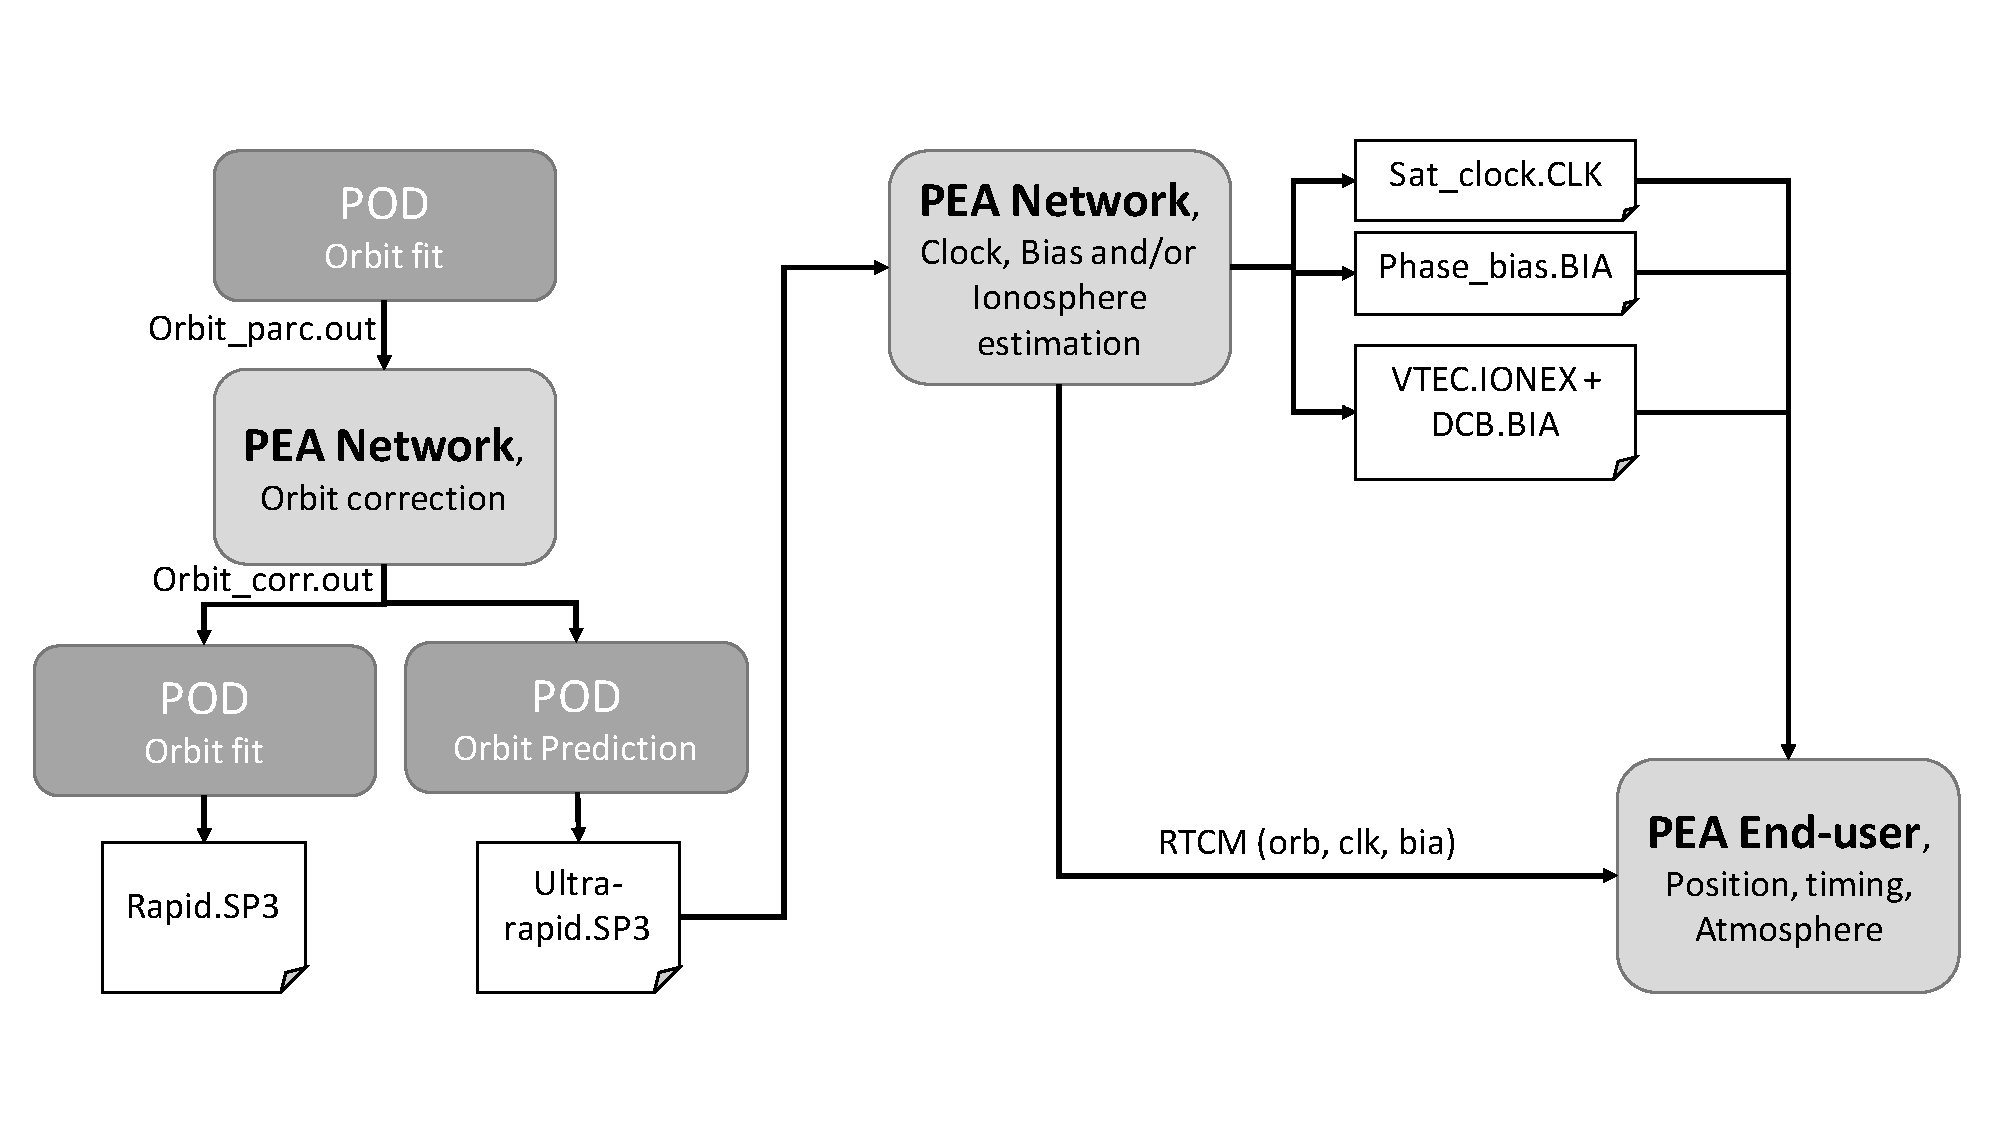
\includegraphics[width=\linewidth]{Figures/Ginan_diagram.pdf}
	\caption{Ginan software components}
	\label{fig:PEAnPOD}
\end{figure}

The software is aimed at supporting Australia's implementation of a national positioning infrastructure that supports the objective of 'instantaneous GNSS positoning anywhere, anytime, with the highest possible accuracy and the highest possible integrity.

\textbf{Carrier phase ambiguity}. The underlying signals transmitted by the Global Navigation Satellite Systems (GNSS) can be considered as waves, just like repeating sine waves from high school mathematics. Measurements of these waves are referred to as carrier phase observations, and they are used to provide the precise distance, with mm precision and accuracy, between the orbiting satellites and user’s receiver that are subsequently used to compute position. However, a complicating factor is that carrier phase observations have an ambiguous component where the total whole number of waves, or integer cycles, between the satellite and the user’s receiver cannot be measured, only the fractional part. The unknown number of integer cycles is called the carrier phase ambiguity. Fortunately, the ambiguities can be estimated, and the mathematical and statistical solution to this problem is known as integer ambiguity estimation. While there is a long history of research in this area, which has largely focused on GPS applications, the most optimal solution to this problem when simultaneously combining data from all the GNSS remains unresolved.

\textbf{Atmosphere delay of GNSS signals}. The Earth is surrounded by layers of gases held by Earth's gravity. Signals, such as those transmitted by GNSS, propagated from space are delayed as they pass through the atmosphere. In the troposphere, the region from the Earth’s surface to approximately 20 km altitude, the delay is proportional to temperature, pressure and humidity. The ionosphere, the region from 50-1000 km altitude, causes delay as a function of the frequency of the signal. The composition of both the troposphere and ionosphere vary both in space and time, and this variability currently limits the accuracy, speed and reliability of positioning. But it’s not all bad news, and like a CAT scan in medical science, the new GNSS signals and satellites can potentially be combined to provide a more complete three dimensional picture of the atmospheric delay as a function of time. Models that more completely remove the nuisance atmospheric signals will lead to improved accuracy, speed and reliability of positioning.

\textbf{Precise Point Positioning (PPP) and Real Time Kinematic (RTK)}. Conventional positioning technologies almost exclusively use a technique called Real Time Kinematic (RTK). The RTK technique takes information from nearby Continuously Operating Reference Stations (CORS) to generate corrections for measurements made by users. One of the most important of these is the carrier phase ambiguity correction. The ability to correctly determine carrier phase ambiguities with RTK is determined by many factors, such as the distance between the reference stations and the user and also atmospheric effects. Consequently, RTK relies on relatively dense CORS networks with a typical spacing of 30 to 70 km. An alternative to RTK is Precise Point Positioning (PPP). The PPP technique, rather than directly using measurements from nearby reference stations, uses global satellite orbit and clock information such as that provided by the International GNSS Service. The major advantage of PPP is that it doesn’t require a dense CORS network nearby the user’s location just access to global products. Unfortunately, the PPP technique can have difficulties in resolving carrier phase ambiguities in real time, but additional research focused on greater exploitation of multi-GNSS data and more regional approaches may in the future overcome this limitation.
	\chapter{Installation}
\label{ch:installation}


In this chapter we will describe how to install the PEA and POD from source. An alternative option to installing all of the dependencies and the source code would be to use one of our docker images available from Docker Hub. Instructions on how to do this are in (see \hyperref[ch:docker]{Docker}).

\section{Supported Platforms}\label{supported-platforms}

Ginan is supported on the following platforms

\begin{itemize}
\item
  Linux
\item
  MacOS\\
\end{itemize}

\section{Download}\label{download}
You can download Ginan source from github using git clone:

\begin{lstlisting}[language=bash]
$ git clone https://github.com/GeoscienceAustralia/ginan.git
\end{lstlisting}

Then download all of the example data using the python script provided:

\begin{lstlisting}[language=bash]
$ python3 scripts/download_examples.py 
\end{lstlisting}


\section{Directory Structure}\label{directory-structure}

\begin{verbatim}
ginan/
├── README.md           ! General README information
├── LICENSE.md          ! Software License information
├── aws/                ! Amazon Web Services config
├── bin/                ! Binary executables directory*
├── CMakeLists.txt      ! Cmake build file
├── docs/               ! Documentation directory
├── examples/           ! Ginan examples directory
│   ├── data/           ! example dataset (rinex files)**
│   ├── products/       ! example products and aux files**
│   ├── solutions/      ! example solutions for QC**
│   --------------PEA examples--------------
│   ├── ex11            ! PEA example 1
│   ├── ex12            ! PEA example 2
│   ├── ex13            ! PEA example 3
│   ├── ex14            ! PEA example 4
│   ├── ex15            ! PEA example 5
│   ├── ex17            ! PEA example 7
│   ├── ex18            ! PEA example 8
│   --------------POD examples--------------
│   ├── ex21            ! POD example 1
│   ├── ex22            ! POD example 2
│   ├── ex23            ! POD example 3
│   ├── ex24            ! POD example 4
│   ├── ex25            ! POD example 5
│   └── ex26            ! POD example 6
│
├── lib/                ! Compiled objectlibrary directory*
├── scripts/            ! Auxillary Python and Shell scripts and libraries
└── src/                ! Source code directory
    ├── cpp/            ! PEA source code
    ├── fortran/        ! POD source code
    ├── cmake/   
    ├── doc_templates/
    ├── build/          ! Cmake build directory*
    └── CMakeLists.txt
\end{verbatim}

\emph{*created during installation process}

\emph{**created by \texttt{download\_examples.py} script}\\


\section{Dependencies}\label{dependencies}

Ginan has several software dependencies:

\begin{itemize}
\item
  C/C++ and Fortran compiler. We use and recommend
  \href{https://gcc.gnu.org}{gcc-g++ and gfortran}
\item
  BLAS and LAPACK linear algebra libraries. We use and recommend
  \href{https://www.openblas.net/}{OpenBlas} as this contains both
  libraries required
\item
  CMAKE \textgreater{} 3.0
\item
  YAML \textgreater{} 0.6
\item
  Boost \textgreater{} 1.70
\item
  Eigen3
\item
  netCDF4
\item
  Python3 (tested on Python 3.7)\\
\end{itemize}

\section{Installing dependencies with Ubuntu}\label{installing-dependencies-with-ubuntu}


Update the base operating system:

\begin{lstlisting}[language=bash]
$ sudo apt update
$ sudo apt upgrade
\end{lstlisting}

Install base utilities \texttt{gcc}, \texttt{gfortran}, \texttt{git},
\texttt{openssl}, \texttt{openblas} etc:

\begin{lstlisting}[language=bash]
$ sudo apt install -y git gobjc gobjc++ gfortran libopenblas-dev openssl curl net-tools openssh-server cmake make libssl1.0-dev
\end{lstlisting}


\section{Building additional
dependencies}\label{building-additional-dependencies}

Depending on the user's installation choice: install PEA-only, POD-only
or all software packages, a set of additional dependencies that need to
be built may change. Below, we explain building all the additional
dependencies:

First, create a temporary directory structure to make the dependencies
in, it can be removed after the installation process is done:

\begin{lstlisting}[language=bash]
$ sudo mkdir -p /data/tmp
$ cd /data/tmp
\end{lstlisting}

Note that \texttt{/data/tmp} is only used here as example and can be any
directory

\begin{itemize}
  

\item \textbf{YAML}
We are using the \href{https://github.com/jbeder/yaml-cpp}{YAML} library
to parse the configuration files used to run many of the programs found
in this library. Here is an example of how to install the yaml library
from source:

\begin{lstlisting}[language=bash]
$ cd /data/tmp
$ sudo git clone https://github.com/jbeder/yaml-cpp.git
$ cd yaml-cpp
$ sudo mkdir cmake-build
$ cd cmake-build
$ sudo cmake .. -DCMAKE\_INSTALL\_PREFIX=/usr/local/ -DYAML\_CPP\_BUILD\_TESTS=OFF
$ sudo make install yaml-cpp
$ cd ../..
$ sudo rm -fr yaml-cpp
\end{lstlisting}

\item\textbf{Boost (PEA)}

PEA relies on a number of the utilities provided by
\href{https://www.boost.org/}{boost}, such as their time and logging
libraries.

\begin{lstlisting}[language=bash]
$ cd /data/tmp/
$ sudo wget -c https://boostorg.jfrog.io/artifactory/main/release/1.73.0/source/boost_1_73_0.tar.gz
$ sudo gunzip boost_1_73_0.tar.gz
$ sudo tar xvf boost_1_73_0.tar
$ cd boost_1_73_0/
$ sudo ./bootstrap.sh
$ sudo ./b2 install
$ cd ..
$ sudo rm -fr boost_1_73_0/ boost_1_73_0.tar
\end{lstlisting}

\item\textbf{Eigen3 (PEA)}

Eigen3 is used for performing matrix calculations in PEA, and has a very
nice API.

\begin{lstlisting}[language=bash]
$ cd /data/tmp/
$ sudo git clone https://gitlab.com/libeigen/eigen.git
$ cd eigen
$ sudo mkdir cmake-build
$ cd cmake-build
$ sudo cmake ..
$ sudo make install
$ cd ../..
$ sudo rm -rf eigen
\end{lstlisting}

\item\textbf{MongoDB (PEA, optional)}

Needed for realtime preview of the processed results (developers-only)

\begin{lstlisting}[language=bash]
$ wget https://github.com/mongodb/mongo-c-driver/releases/download/1.17.1/mongo-c-driver-1.17.1.tar.gz
$ tar -xvf mongo-c-driver-1.17.1.tar.gz

$ cd mongo-c-driver-1.17.1/
$ mkdir cmakebuild
$ cd cmakebuild/
$ cmake -DENABLE_AUTOMATIC_INIT_AND_CLEANUP=OFF ..
$ cmake --build .
$ sudo cmake --build . --target install

$ cd ../../
$ curl -OL https://github.com/mongodb/mongo-cxx-driver/releases/download/r3.6.0/mongo-cxx-driver-r3.6.0.tar.gz
$ tar -xzf mongo-cxx-driver-r3.6.0.tar.gz

$ cd mongo-cxx-driver-r3.6.0/

$ cd build/
$ cmake -DCMAKE_BUILD_TYPE=Release -DCMAKE_INSTALL_PREFIX=/usr/local ..
$ sudo cmake --build . --target EP_mnmlstc_core
$ cmake --build .
$ sudo cmake --build . --target install

$ wget -qO - https://www.mongodb.org/static/pgp/server-4.4.asc | sudo apt-key add -
$ echo "deb [ arch=amd64,arm64 ] https://repo.mongodb.org/apt/ubuntu focal/mongodb-org/4.4 multiverse" | sudo tee /etc/apt/sources.list.d/mongodb-org-4.4.list
$ echo "deb [ arch=amd64,arm64 ] https://repo.mongodb.org/apt/ubuntu bionic/mongodb-org/4.4 multiverse" | sudo tee /etc/apt/sources.list.d/mongodb-org-4.4.list

$ sudo apt update
$ sudo apt install mongodb-org 

$ sudo systemctl start mongod
$ sudo systemctl status mongod
$ mongod
\end{lstlisting}

\item\textbf{netcdf4 (OTL package)}

\begin{lstlisting}[language=bash]
$ sudo apt -y install libnetcdf-dev libnetcdf-c++4-dev
\end{lstlisting}

\end{itemize}

\section{Build}\label{build}

Prepare a directory to build in, its better practise to keep this
seperated from the source code.

\begin{lstlisting}[language=bash]
$ cd src
$ mkdir -p build
$ cd build
\end{lstlisting}

Run cmake to find the build dependencies and create the make file. If
you wish to enable the optional MONGO DB utilities you will need to add
the \texttt{-DENABLE\_MONGODB=TRUE} flag. If you wish to compile an
optimised version, typically this version will run 3 times faster but
you may run into compile problems depending on your system, add the
\texttt{-DOPTIMISATION=TRUE} flag:

\begin{lstlisting}[language=bash]
$ cmake [-DENABLE_MONGODB=TRUE] [-DENABLE_OPTIMISATION=TRUE] ..
\end{lstlisting}

To build every package simply run \texttt{make} or \texttt{make\ -j\ 2},
where 2 is a number of parallel threads you want to use for the
compilation:

\begin{lstlisting}[language=bash]
$ make [-j 2]
\end{lstlisting}

To build specific package (e.g.~PEA or POD), run as below:

\begin{lstlisting}[language=bash]
$ make pea -j 2
$ make pod -j 2
\end{lstlisting}

This should create executables in the \texttt{bin} directory of Ginan.

Check to see if you can execute the PEA:

\begin{lstlisting}[language=bash]
$ ../../bin/pea --help
\end{lstlisting}

and you should see something similar to:

\begin{lstlisting}[language=bash]
PEA starting... (pea_pod_examples vbf8c9cc from Tue Jul 6 06:09:50 2021)
Options:
--help                      Help
--quiet                     Less output
--verbose                   More output
--very-verbose              Much more output
--config arg                Configuration file
--trace_level arg           Trace level
--antenna arg               ANTEX file
--navigation arg            Navigation file
--sinex arg                 SINEX file
--sp3files arg              Orbit (SP3) file
--clkfiles arg              Clock (CLK) file
--dcbfiles arg              Code Bias (DCB) file
--bsxfiles arg              Bias Sinex (BSX) file
--ionfiles arg              Ionosphere (IONEX) file
--podfiles arg              Orbits (POD) file
--blqfiles arg              BLQ (Ocean loading) file
--erpfiles arg              ERP file
--elevation_mask arg        Elevation Mask
--max_epochs arg            Maximum Epochs
--epoch_interval arg        Epoch Interval
--rnx arg                   RINEX station file
--root_input_dir arg        Directory containg the input data
--root_output_directory arg Output directory
--start_epoch arg           Start date/time
--end_epoch arg             Stop date/time
--run_rts_only arg          RTS filename (without _xxxxx suffix)
--dump-config-only          Dump the configuration and exit
--input_persistance         Begin with previously stored filter and 
                            navigation states
--output_persistance        Store filter and navigation states for restarting
PEA finished
\end{lstlisting}

Similarly, check the POD:

\begin{lstlisting}[language=bash]
$ ../../bin/pod --help
\end{lstlisting}

This returns:

\begin{lstlisting}[language=bash]
Earth Radiation Model (ERM):   1

Default master POD config file = POD.in
To run from default config file: ../../bin/pod or ../../bin/pod -c POD.in

POD.in config file options by defaut can be overridden on the command line

Command line: ../../bin/pod -m -s -o -a -p -r -t -n -i -u -q -k -w -y -h 

Where: 
    -m --podmode = POD Mode:
                                1 - Orbit Determination (pseudo-observations; orbit fitting)
                                2 - Orbit Determination and Prediction
                                3 - Orbit Integration (Equation of Motion only)
                                4 - Orbit Integration and Partials (Equation of Motion and Variational Equations)
    -s --pobs    = Pseudo observations orbit .sp3 file name
    -o --cobs    = Comparison orbit .sp3 file name
    -a --arclen  = Orbit Estimation Arc length (hours)
    -p --predlen = Orbit Prediction Arc length (hours)
    -r --eopf    = Earth Orientation Paramaeter (EOP) values file
    -t --eopsol  = Earth Orientation Paramaeter file type: (1,2,3)
                                1 - IERS C04 EOP
                                2 - IERS RS/PC Daily EOP
                                3 - IGS RP + IERS RS/PC Daily (dX,dY)
    -n --nutpre  = IAU Precession / Nutation model
                                2000 - IAU2000A
                                2006 - IAU2006/2000A
    -i --estiter = Orbit Estimatimation Iterations (1 or greater)
    -u --sp3vel  = Output .sp3 file with velocities
                                0 - Do not write Velocity vector to sp3 orbit
                                1 - Write Velocity vector to sp3 orbit
    -q --icmode  = Initial condition from parameter estimation procedure
    -k --srpmodel= 1: ECOM1, 2:ECOM2, 12:ECOM12, 3:SBOX
    -w --empmodel= 1: activated, 0: no estimation
    -d --verbosity = output verbosity level [Default: 0]
    -y --yaml = yaml config file
    -h --help.   = Print program help

Examples:

        ../../bin/pod -m 1 -q 1 -k 1 -w 0 -s igs16403.sp3 -o igs16403.sp3 -y ex1.yaml
        ../../bin/pod -m 2 -q 1 -k 1 -w 0 -s igs16403.sp3 -p 12 -y ex2.yaml

For orbit updates using Parameter Estimation Algorithm (PEA):
        ../../bin/pod -m 4 -q 2 -k 1 -w 0 -s igs16403.sp3 -o igs16403.sp3 -y ex3.yaml
\end{lstlisting}


\section{Documentation}\label{documentation}

Ginan documentation consists of two parts: a doxygen-generated
documentation that shows the actual code infrastructure and a detailed
manual, written in latex, that provides an overview of the software, a
thoretical background, a detailed ``how to'' guide etc.\\
Below, we explain on how to generate each bit of documentation:

\subsection{Doxygen}\label{doxygen}

The Doxygen documentation for Ginan requires \texttt{doxygen} and
\texttt{graphviz}. If not already installed, type as follows:

\begin{lstlisting}[language=bash]
$ sudo apt -y install doxygen graphviz
\end{lstlisting}

On success, proceed to the build directory and call make with
\texttt{doc\_doxygen} target:

\begin{lstlisting}[language=bash]
$ cd src/build
$ make doc_doxygen
\end{lstlisting}

The docs can then be found at \texttt{docs/html/index.html}. Note that
documentation is generated automatically if \texttt{make} is called
without arguments and \texttt{doxygen} and \texttt{graphviz}
dependencies are satisfied.

\subsection{Latex}\label{latex}

A detailed Ginan manual is located in \texttt{docs/manual} and is in
latex format. To compile Latex to pdf you will need a compiler, such as
texlive:

\begin{lstlisting}[language=bash]
$ sudo apt install texlive-latex-base texlive-latex-extra
\end{lstlisting}

Now, go to \texttt{docs/manual} and generate the pdf:

\begin{lstlisting}[language=bash]
$ cd docs/manual
$ pdflatex main.tex
$ makeglossaries main
$ pdflatex main.tex
\end{lstlisting}

\texttt{main.pdf} file should now appear in the directory.\\


\section{Ready!}\label{ready}

Congratulations! You are now ready to trial the examples of PEA and POD
from the examples directory. See Ginan's manual for detailed explanation
of each example. Note that examples have relative paths to files in them
and rely on the presence of \texttt{products}, \texttt{data} and
\texttt{solutions} directories inside the \texttt{examples} directory.
Make sure you've run \texttt{download\_examples.py} from the
\hyperref[download]{download} step of this instruction.

The paths are relative to the examples directory and hence all the
examples must be run from the \texttt{examples} directory.

\begin{lstlisting}[language=bash]
cd ../../examples
\end{lstlisting}

To run the first example of the PEA:

\begin{lstlisting}[language=bash]
../bin/pea --config ex11_pea_pp_user_gps.yaml
\end{lstlisting}

This should create \texttt{ex11} directory with
\texttt{ex11-ALIC201919900.TRACE} and \texttt{ex1120624.snx} output
files. You can remove the need for path specification to the executable
by adding Ginan's bin directory to \texttt{\textasciitilde{}/.bachrc}
file:

\begin{lstlisting}[language=bash]
PATH="path_to_ginan_bin:$PATH"
\end{lstlisting}

And an example of POD:

\begin{lstlisting}[language=bash]
../bin/pod -y ex21_pod_fit_gps.yaml
\end{lstlisting}

At the completion of the test run, \texttt{ex21} directory should be
create. The \texttt{ex21\_.sh} script will return any differences to the
standard test resuts.


\section{Python Installation for Plotting, Processing,
etc.}\label{python-installation-for-plotting-processing-etc.}

Lastly, to run many of the included scripts for fast parsing of
.trace/.snx files, plotting of results, automatic running of the PEA
based on input date/times and stations, etc. then a number of python
dependencies are needed.

The file scripts/conda\_gn37.yaml has a list of the necessary python
dependencies.\\
The best way to take advantage of this is to install the Miniconda
virtual environment manager.\\
This will allow you to pass the .yaml file into the conda command and
automatically set up a new python environment.

\begin{enumerate}
  \item\textbf{Install Miniconda}

To install Miniconda, download and execute the Miniconda shell file:

\begin{lstlisting}[language=bash]
$ wget https://repo.anaconda.com/miniconda/Miniconda3-latest-Linux-x86_64.sh
$ bash Miniconda3-latest-Linux-x86_64.sh
\end{lstlisting}

And follow the on-screen instructions (choosing all defaults is fine).

\item\textbf{Create virtual
environment}

After installation you can create the \texttt{gn37} python environment
using a prepared receipy. First open a new terminal session and enter:

\begin{lstlisting}[language=bash]
$ conda env create -f <dir_to_ginan>/scripts/conda_gn37.yaml
\end{lstlisting}

\end{enumerate}

You have now created the virtual python environment \texttt{gn37} with
all necessary dependencies. Anytime you wish you run python scripts,
ensure you are in the virtual environment by activating:

\begin{lstlisting}[language=bash]
$ conda activate gn37
\end{lstlisting}

And then run your desired script from the \texttt{scripts} directory.
	%\include{implementation overview of software}
	% % block diagram from aaron
	\chapter{PEA examples}
\label{ch:pea_examples}

In this section we go through a number of different ways that the pea can be used to process GNSS data.
\begin{enumerate}
	\item Precise Point Positioning (PPP) processing - In this section we will demonstrate how to processing in PPP mode using the Ionosphere free combination, we will provide an example on how to use IGS products to obtian a float solution, and then an example on how to obtain an ambguity fixed solution. We will also cover how to process gnss streams in realtime.
	\item Obtain an orbit solution from a global tracking network
	\item Obtain an orbit and clock solution from a global tracking network
	\item How to process a Global solution in real-time
	\item How to obtain an ionosphere model 
\end{enumerate}
%


	\chapter{POD Examples}
\label{ch:pod_examples}

\section{Processing Example 1}
In this example the pod will perform a dynamic orbit determination for PRN04 over a 6 hour arc. 
The full gravitational force models are applied, with a cannonball model SRP model.

To run the POD ...
\begin{lstlisting}
$ bin/pod
\end{lstlisting}

This should output the following to stdout...
\begin{lstlisting}
Orbit Determination
Orbit residuals in ICRF : RMS(XYZ)   1.6754034501980351E-002   5.2908718335411935E-002   1.5676115599034774E-002
Orbit Determination: Completed
CPU Time (sec)   298.48134399999998
External Orbit comparison
Orbit comparison: ICRF
RMS RTN   2.8094479714173427E-002   2.4358145601708528E-002   4.4097979280889953E-002
RMS XYZ   1.6754034501980351E-002   5.2908718335411935E-002   1.5676115599034774E-002
Orbit comparison: ITRF
RMS XYZ   3.9069978513805753E-002   3.9343671258381237E-002   1.5660654272651970E-002
Write orbit matrices to output files
CPU Time (sec)   349.19307899999995
The results above show that our orbits arcs, over 6 hours, are currently within 2-5 cm of the final combined IGS orbit.
\end{lstlisting}

The processing also produces the following output files...
\begin{verbatim}
%├── DE.430            planetary ephemris intermediate file
%├── Amatrix.out       design matrix
%├── Wmatrix.out       reduced observation matrix
%├── orbext_ICRF.out   intermediary file for the IGS orbit solution in ICRF for comparison purposes
%├── orbext_ITRF.out   intermediary file for the IGS orbit solution in ITRFfor comparison purposes
%├── dorb_icrf.out     differences in solutions in ICRF
%├── dorb_RTN.out      differences in solutions in orbital frame components radial, tangential and normal (RTN)
%├── dorb_Kepler.out   differences in solutions in keperian elements 
%├── dorb_itrf.out     differences in solutions in ITRF 
%├── orb_icrf.out      the final estimated orbit in ICRF
%├── orb_itrf.out      the final estimated orbit in ITRF
%├── VEQ_Smatrix.out   State transition matrix from the variational equations solution
%├── VEQ_Pmatrix.out   Sensitivity matrix from the variational equations solution
\end{verbatim}

\section{Processing Example 2 - ECOM2 SRP}
In this example we will change the SRP model to use the ECOM2 model.

Edit the EQM.in file so that the Solar Radiation Pressure configuration section now looks:

! Solar Radiation Pressure model: ! 1. Cannonball model ! 2. Box-wing model ! 3. ECOM (D2B1) model SRP\_model 3

Then edit VEQ.in, so that the Non-gravitational forces now looks like:

%% Non-gravitational Effects Solar_radiation 0 Earth_radiation 0 Antenna_thrust 0

! Solar Radiation Pressure model: ! 1. Cannonball model ! 2. Box-wing model ! 3. ECOM (D2B1) model SRP\_model 3

run the POD ...

\begin{lstlisting}
$ bin/pod
\end{lstlisting}
This should output the following to stdout...
\begin{lstlisting}
Orbit Determination
Orbit residuals in ICRF : RMS(XYZ)   2.0336204859568077E-002   8.4715644601919167E-003   3.9687932322714677E-002
Orbit Determination: Completed
CPU Time (sec)   299.68054799999999
External Orbit comparison
Orbit comparison: ICRF
RMS RTN   2.8182836396022540E-002   2.4598832384842121E-002   2.5879201921952168E-002
RMS XYZ   2.0336204859568077E-002   8.4715644601919167E-003   3.9687932322714677E-002
Orbit comparison: ITRF
RMS XYZ   1.8757217704973204E-002   1.1635302426688266E-002   3.9702619816620370E-002
Write orbit matrices to output files
CPU Time (sec)   350.88653299999999\
\end{lstlisting}

\section{Example 3 - (pod/examples/ex3)}
GPS IGS SP3 file orbit fitting, orbit prediction and comparison to next IGS SP3 file

\section{Example 4 - (pod/examples/ex4):}
Integration of POD initial conditions file generated by the PEA

\section{Example 5 - (pod/examples/ex5):}
ECOM1+ECOM2 hybrid SRP model
In each example directory (ex1/ex2/ex3/ex4) there is a sh\_ex? script that when executed will run the example and compare the output with the expected solution.

\textit{The POD} is designed to do some stuff.
	% %
	\part{Background Theory}
	\chapter{GNSS Overview}
\label{ch:GNSSOverview}

\section{GPS}

\section{Glonass}

\section{Galileo}

\section{Beidou}

\section{QZSS}

\textbf{The \index{PEA} and POD} is designed to do some stuff.
	\chapter{Equation Conventions}
\label{ch:conventions}

\textit{In this manual we will} be adhering to the following conventions

\section{List of Symbols}

\begin{itemize}
	\item {\boldmath{$i$}} Receiver identification or {\boldmath{$r$}}
	\item {\boldmath{$j$}} Satellite identification or {\boldmath{$s$}}
	\item {\boldmath{$k$}} Epoch number or {\boldmath{$t$}}
	\item {\boldmath{$q$}} GNSS type (GPS,GALILEO,GLONASS,QZSS)
	\item {\boldmath{$c$}} Speed of light [m/s]
	\item {\boldmath{$x$}} Vector of parameters to be estimated
	\item {\boldmath{$y$}} Vector of observations
	\item {\boldmath{$v$}} Vector of residuals
	\item {\boldmath{$H$}} Design matrix
	\item {\boldmath{$\sigma$}} Standard deviation of observable
	\item {\boldmath{$\Delta$}} Increment to a priori values [m]
	\item {\boldmath{$\lambda$}} Wavelength or {\boldmath{$\lambda_1,\lambda_2,\lambda_5$}}
	\item {\boldmath{$f_1,f_2,f_5$}} frequency
	\item {\boldmath{$\alpha$}} Ambguity or {\boldmath{$N$}} Real valued ambguity and {\boldmath{$\bar{N}$}} Integer part of real valued ambguity
	\item {\boldmath{$\alpha$}} level of significance
	
	\item {\boldmath{$\beta$}} Biases
	\item {\boldmath{$\zeta$}} Clock offsets
	\item {\boldmath{$\delta t$}} Clock error [s]
	\item {\boldmath{$\kappa$}} Correction - relativity
	\item {\boldmath{$\iota$}} Ionosphere or  {\boldmath{$I$}}
	\item {\boldmath{$\tau$}} Troposphere or {\boldmath{$T,T_h,T_w$}}
	\item {\boldmath{$M$}} elevation dependent mapping function for the troposphere wet delay
	\item {\boldmath{$\xi$}} Phase wind-up error
	\item {\boldmath{$\epsilon$}} Error in observations and unmodelled effects [m]
	\item {\boldmath{$\phi_i^j$}} Carrier phase observable (times c) [m]
	\item {\boldmath{$P_i^j$}} Pseudo range observable [m]
		
\end{itemize}

Lets try this for example:
For an undifference, uncombined float solution, the linearized observation equations for pseudorange and phase observations from satellite $s$ to receiver $r$ can be described as:

\begin{math}
\Delta P_{r,f}^{q,s} = u_r^{q,s} . \Delta x + c . (\delta t_r^q - \delta t^{q,s}) + M_r^{q,s} . T_r + \gamma_f^q . I_{r,1}^{q,s} + d_{r,f}^q - d_f^{q,s} + \epsilon_{P,f}^q
\end{math}\\
\begin{math}
\Delta\phi_{r,f}^{q,s} = u_r^{q,s} . \Delta x + c . (\delta t_r^q - \delta t^{q,s}) + M_r^{q,s} . T_r - \gamma_f^q . I_{r,1}^{q,s} + \lambda_f^q . N_{r,f}^{q,s} + b_{r,f}^q - b_f^{q,s} + \epsilon_{L,f}^q 
\end{math}

where$\Delta P_{r,f}^{q,s}$ and $\Delta\phi_{r,f}^{q,s}$ are the respective pseudorange and phase measurements on the frequency $f$(f=1,2), from which the computed values are removed;
$u_r^{q,s}$ is the receiver-to-satellite unit vector;
$\Delta x$ is the vector of the receiver position corrections to its preliminary position; 
$\delta t_r^q$ and $\delta t^{q,s}$ are the receiver and satellite clock errors respectively;
$c$ is the speed of light in a vaccum
$M_r^{q,s}$ is the elevation dependent mapping function for the troposphere wet delay from the corresponding zenith one $T_r$;
$I_{r,1}^{q,s}$ is the ionosphere delay along the line-of-sight from a receiver to a satellite at the first frequency and $\gamma_f^q = (\lambda_f^q / \lambda_1^q)^2$;
$\lambda_f^q$ is the wavelength for the frequency $f$ of a GNSS $q$;
$N_{r,f}^{q,s}$is the phase ambguity 
$d_{r,f}^q$ and $b_{r,f}^q$ are the receiver hardware delays of code and phase observations respectively;
$d_f^{q,s}$ and $b_f^{q,s}$ are the satellite hardware delays of code and phase observations, respectively;
$\epsilon_{P,f}$ and $\epsilon_{L,f}$ are the code and phase measurement noises respectively. 


	\chapter{Observation Modelling}
\label{ch:observation_modelling}

\section{Ionosphere-Free Observations}

\section{Undifferenced - Uncombined}
To do ..
\textit{The PEA and POD} is designed to do some stuff.

\section{GPS Quarter Cycle}
The $L_2$ Civil code (L2C-code) is shifted by a quarter cycle with respect to the P-code. If a receiver is using either the one or the other code to reconstruct the carrier phase measurements, then they will also be shifted by a quarter of a wavelength relative to each other.\\
The noise of phase measurement based on L2C-code is usually lower than the noise of phase observations reconstructed based on p-code. However this is only possible to obtain from satellites that have launched since GPS Block IIR-M was deployed. Older GPS satellites do not provide the L2C-code signal.\\
In RINEX version 2, in order to prevent potential problems in ambiguity resolution some receiver manufactures do correct the phase measurements by 0.25 cycles to keep the phase observations consistent, while others provide the uncorrected phase measurements, an din other cases the user can decide if the correction is applied. Since RINEX version 3.02 the definition has been defined that the phase measurements need to be corrected to have a consistent set of observable that can be introduce for ambiguity resolution.\\
One option to prevent having the quarter cycle issue is to ensure that ambiguities are not resolved between a Block IIR-M or later  with an older satellite.

\section{Single-satellite and Single-Receiver Observation Combinations}

Linear combinations of the original observations are often applied to eliminate model parameters (eg ionosphere slant delays) or to transform ambiguity parameters (eg widelane transformation). Some of these transformations maintain the information content of the system as they are invertible, but other transformation that are used are do not, and these should be used with caution as the information that contributes to the parameters of interest are lost.\\
%
A large number of different permutations of linear combinations can be formed, with just the dual-frequency legacy signals, this can increases even more as more additional frequencies are available with modernized GNSS signals are deployed. We will only cover the ones used by the PEA in this manual.\\
%
Combining two or more carrier-phase observations into a new signal leads to a different frequency/wavelength. To generalise in the case of a combination for which $\sigma \alpha = 1$, the combined frequency $f_c$ is:
\begin{equation}
f_c = \sigma_{j=1}^n i_j f_j 
\label{eq:comb_freq}
\end{equation}

Remembering that all frequencies for GNSS are derived from a single frequency $f_0$ by multiplication with an integer $k_j$, the individual frequency is obtained from $f_j = j_jf_0$. substituting this into the above equation

$f_c = (\sigma_{j=1}^n i_j k_j) = kf_0$ \label{eq:}

where $k$ is the \emph{lane number}. The corresponding wavelength is:

$\lambda_c = c / kf_0 = \lambda_0 / k$ 

where $\lambda_0$ is the wavelength of the base frequency $f_0$. Since all $i_j$ and $k_j$ are integers, $k$ is also an integer. This parameter uniquely defines the frequency and wavelength of the new signal combination.

With the help of the lane number $k$, the combinations can be categorized into three groups:
\begin{enumerate}
    \item \emph{wide-lane} combination,where the combined wavelength is larger than the largest individual wavelength in the combination.
    \item \emph{intermediate} combinations, for which $\lambda_0$ leas between the largest and shortest individual wavelength.
    \item \emph{narrow-lane} combinations which have a shorter wavelength than the individual signal with the shortest wavelength in the combination.
\end{enumerate}

\textit{The zero-differenced}, ionosphere free mathematical model for code and phase measurements using dual-frequency can be described by:\\

$ E(P_{r,IF}^S) = \rho_{r}^s + c(dt_{r} - dt^s) + \tau_r^s + c (d_{r,IF} + d_{r,IF}^s) $\label{eq:code_IF_eq}\\

$ E(L_{r,IF}^S) = \rho_{r}^s + c(dt_{r} - dt^s) + \tau_r^s + \lambda_{IF} (z_{r,IF}^s + \delta_{r,IF} - \delta_{IF}^S$\label{eq:phase_IF_eq}\\

with:

$E()$ the expectation notation
$P_{r,IF}^S$ code measurements (m) between satellite $s$ and receiver $r$ for the ionosphere-free measurements;\\
$L_{r,IF}^S$ phase measurements (m)\\
$\rho$ the geometric distance (m)\\
$c$ speed of light (m/s)\\
$dt_r$ receiver clock error (s)\\
$dt^S$ satellite clock error (s)\\
$\tau_r^s $ slant troposphere delay between satellite s and receiver r (m)\\
$dt_{r,IF}$ receiver code bias (s)\\
$dt_{IF}^S$ satellite code bias (s)\\
$\lambda_{IF}$ ionosphere-free wavelength (m)\\
$z_{r,IF}^S$ ionosphere-free ambiguity vector (cycle)\\
$\delta_{r,IF}^S$ receiver ionosphere-free phase bias (cycle)\\
$\delta_{IF}^S$ satellite ionosphere-free phase bias (cycle)\\
%
The ionosphere-free combination will remove the first-order ionosphere delay, both equations are rand deficient and the ambiguity term in eq (2) is not an integer. In order to resolve the ambiguities the linear dependency among the unknown parameters needs to be resolved and the integer property of the ambiguities needs to be recovered. 

\section{Widelane combinations}
The group of wide-lane combinations is especially useful to help with integer ambiguity resolution due to their longer wavelength.

%\begin{figure*}[h]
%\includegraphics[]{images/widelane.png}
%  \caption{Illustration of the linear widelane combinations. Two original frequencies (top and middle) are subtracted to form a longer wavelength observable (bottom)}%
%  \label{fig:widelane}%
%\end{figure*}



\subsection{Common widelane}
To improve ambiguity resolution, often the wide lane linear combination (also called L5 or LW linear combination) is formed from the L1 and L2 carrier phase observables. It is designed to be a geometry-preserving combination using only carrier-phase measurements in the frequencies $f_a$ and $f_b$. By selecting the integer coefficients as $i_A = +1$ and $i_B = -1$, one obtains the WL carrier-phase combination $\phi_{r,WL}^s$ in units of cycles:
\begin{equation}
\phi_{r,WL}^s = \phi_{r,A}^A - \phi_{r,B}^S = \frac{\psi_{r,A}^s}{\lambda_A} - \frac{\psi{r,B}^s}{\lambda_B} \label{eq:wl_cycles}
\end{equation}

The corresponding wavelength $\lambda_{WL}$ is:
\begin{equation}
\lambda_{WL} = \frac{c}{f_A - f_B} 
    \label{eq:wl_wavelength}
\end{equation}

Multiplication of the two above equations leads to the wide-lane combination $\psi_{r,WL}^s$ in units of meters:
\begin{equation}
\psi_{r,WL}^S = \frac{f_A}{f_A-f_B}\psi_{r,A}^s - \frac{f_B}{f_A-f_B}\psi_{r,B}^s
\end{equation}

\subsection{Melbourne-Wubbena linear combination}
The Melbourne-Wubbena linear combination (Melbourne 1985),(Wubbena 1985) is a linear combination of the L1 and L2 carrier phase plus the P1 and P2 pseudorange. The geometry, troposphere and ionosphere are eliminated by it. The Melbourne-Wubbena linear combination can be represented as:

$
E(L_{r,IF}^S) - \frac{cf_2z_{r,w}^s}{f_1^2 - f_2^2} = \rho_r^s + c(dt_{r,IF} - dt_{IF}^s) + \tau_r^s + \lambda_n z_{r,1}^s + (\lambda_{IF}\delta_{r,IF}$

Since ,,% comprises of both code and phase measurements, it is reasonable to exclude the lower
elevation measurements to avoid the multipath impacts from the code observation. Normally, with
30 degree elevation cut-off, an averaging of 5 minutes of (4) is good enough to fixing the wide-lane
ambiguities [RD 04]. The rests are the wide-lane phase bias, which can be broadcasted to the user for
user side wide-lane ambiguity resolution. Either choosing a pivot receiver bias or a single-differencing
between two satellites can avoid the linear dependency. 


-doesn't need lambda not as correlated
	\chapter{Kalman Filtering}
\label{ch:kalman_filter}
%
The Kalman filter is over 50 years old but is still one of the most important and common data fusion algorithms in use today. 
Named after Rudolf E.Kálmán, the great success of the Kalman filter is due to its small computational requirement, elegant recursive properties, and its status as the optimal estimator for one-dimensional linear systems with Gaussian error statistics. 
Typical uses of the Kalman filter include smoothing noisy data and providing estimates of parameters of interest. 
Kalman filtering is used in a wide range of applications include global positioning system receivers, in control systems, through to the smoothing the output from laptop trackpads, and many more.

\section{Overview of Kalman Filtering}

Kalman filter are typically used to estimate parameters which change with time. 
Parameters with no process noise are called deterministic.
A Kalman filter has measurements $y_t$, with noise $y_t$, and a state vector $\hat x_t$ (or a parameter list) which have specified statistical properties.

The observation equation at time t:
\begin{equation}
    y_t = H_t x_t + \epsilon_t	 \label{eq:kfObs}
\end{equation}

The state transition equation:
\begin{equation}
    x_{t+} = F_t x_t + w_t	
\end{equation}

The kalman filter processing is broken up into three main steps.

\textit{Prediction} {uses a process noise model} to 'predict' the parameters at the next data epoch, subscript is time quantity refers to, where as the superscript refers to the time of the data:
\begin{equation}
    \hat{x}_{t+1}^t = F_t \hat{x}_t^t
\end{equation}
where, $F_t$ is the state transition matrix
\begin{equation}
    P_{t+1}^t = F_t P_t^t F_t^\intercal + Q_t
\end{equation}
where, $Q_t$ is the process noise covariance matrix.
The state transition matrix $F$ projects the state vector (parameters) forward to the next epoch.
\begin{itemize}
    \item For random walk $F$ = 1
    \item For rate terms: $F$ is matrix 
    $\begin{bmatrix}
    1 & \delta t\\
    0 & 1
  \end{bmatrix}$
    \item for FOGM: $F$ = $e^{-\delta t \beta}$
    \item For white noise $F$ = 0
\end{itemize}
The second equation projects the covariance matrix of the state vector, $P$, forward in time. Contributions from the state transition and process noise ($Q$ matrix). 
$Q$ elements are 0 for deterministic parameters.
%
\textit{The Kalman gain} {is the matrix} that allocates the differences between the observation at time t+1 and their predicted value at this time based on the current values of the state vector according to the noise in the measurements and the state vector noise.

\section{Comparison between Weighted Least Squares and Kalman Filtering}

\begin{itemize}
    \item In kalman filtering apriori constraints must be give for all parameters. This is not needed in weighted least squares, but can also be done.
    \item Kalman filters can allow for 0 variance parameters, this cannot be done in WLS, as this requires the inversion of the constraint matrix.
    \item Kalman filter can allow for a method of applying absolute constraints, WLS can only tightly constrain parameters.
    \item Kalman filters are more prone to numerical stability problems, and take longer to run (they have more parameters).
    \item Process noise models can be implemented in WLS, but they are computationally slow.
\end{itemize}

\section{Implementation in the PEA}

\subsection{Robust Kalman Filter Philosophy}

It is well known that the Kalman filter is the optimal technique for estimating parameters of interest from sets of noisy data - provided the model is appropriate.

In addition, statistical techniques may be used to detect defects in models or the parameters used to characterise the data, providing opportunities to intervene and make corrections to the model according to the nature of the anomaly.

By incorporating these features into a single generic module, the robustness that was previously available only under certain circumstances may now be automatically applied to all systems to which it is applied. These benefits extend automatically to all related modules (such as RTS), and often perform better than modules designed specifically to address isolated issues.

\subsection{Initialisation}

When parameters' initial values are not known a-priori, it is often possible to determine them using a least-squares approach.

To minimise processing times, the minimal subset of existing states, measurements, and covariances are used in least-squares estimation whenever the initial value and variance of a parameter is unspecified.

For rate parameters, multiple epoch’s worth of data are required for an ab-initio initialisation. This logic is incorporated into the filter and is applied automatically as required.

\subsection{Outlier detection, Iteration, and Hypothesis Testing}

As a statistical machine, the Kalman filter is capable of detecting measurements that do not fit within the system as modelled.

In these cases, the model may be adjusted on-the-fly, to allow all measurements to be continued to be used without contaminating the results in the filter.

A typical example of a modelling error in GNSS processing is a cycle-slip, in which the ambiguity term (which usually modelled with no change over time) has a discontinuity. Other examples may include clock-jumps or satellite burns.

Hypotheses are to be generated for any measurements that are statistical outliers, and the model iterated as required.

\subsection{Performance Optimisation}

The inversion of large matrices as required by the Kalman filter easily dominates the processing time required during operation. Techniques are available to reduce, and distribute this processing burden across multiple processors.

The Eigen library is used for algebraic manipulation which allows for automatic parallelisation of vector algebra, and improves code robustness by checking matrix dimensions while in use.

\subsubsection{Chunking}

By dividing measurements into multiple smaller sub-matrices, the long inversion times may be reduced, as the inversion order is of $O(n^3)$

\subsubsection{Blocking}
By separating the filter covariance matrix into a block-diagonal form, individual blocks of the filter may be processed individually, without degredation in accuracy. This may improve performance, and may also enable blocks that are relatively independent to be processed separately, albeit with some degredation in accuracy.

\section{Configuration} \label{KFConfig}

All elements within the kalman filter are configured using the yaml configuration file, and use a consistant format.

\subsection{default\_filter\_parameters}

\begin{lstlisting}[language=yaml,caption=Filter Parameters:]

default_filter_parameters:

    stations:

        error_model:        elevation_dependent         #uniform elevation_dependent
        code_sigmas:        [0.15]
        phase_sigmas:       [0.0015]

        pos:
            estimated:          true
            sigma:              [0.1]
            proc_noise:         [0] #0.57 mm/sqrt(s), Gipsy default value from slow-moving
            proc_noise_dt:      second
            #apriori:                                   # taken from other source, rinex file etc.
            #frame:              xyz #ned
            #proc_noise_model:   Gaussian

        clk:
            estimated:          true
            sigma:              [0]
            proc_noise:         [10]
            proc_noise_dt:      second
            #proc_noise_model:   Gaussian

        clk_rate:
            estimated:          false
            sigma:              [500]
            proc_noise:         [1e-4]
            proc_noise_dt:      second
            clamp_max:          [+500]
            clamp_min:          [-500]
            
    satellites:

        clk:
            estimated:          true
            sigma:              [1000]
            proc_noise:         [1]
            #proc_noise_dt:      min
            #proc_noise_model:   RandomWalk

        # clk_rate:
        #     estimated:          true
        #     sigma:              [10]
        #     proc_noise:         [1e-5]
        #     # clamp_max:          [+500]
        #     # clamp_min:          [-500]

        orb:
            estimated:          false

    eop:
        estimated:  true
        sigma:      [40]


override_filter_parameters:

    stations:
        #ALIC:
            pos:
                sigma:              [0.001]
                proc_noise:         [0]
\end{lstlisting}


The majority of estimated states are configured in this section. These configurations are applied to all estimates unless another configuration overrides these parameters in the override\_filter\_parameter section.

The parameters that are available for estimation include:
\begin{itemize}
\item stations:
\begin{itemize}
\item pos
\item pos\_rate
\item clk
\item clk\_rate
\item amb
\item trop
\item trop\_grads
\end{itemize}
\item satellites:
\begin{itemize}
\item pos (coming soon)
\item pos\_rate (coming soon)
\item clk
\item clk\_rate
\item orb
\end{itemize}
\end{itemize}


\subsection*{estimated:}

Boolean to add the state(s) to the kalman filter for estimation.

\subsection*{sigma:}

List of a-priori sigma values for each of the components of the state.

If the sigma value is left as zero (or not initialised), then the initial variance and value of the state will be estimated by using a least-squares approach.
In this case, the user must ensure that the solution is likely rank-sufficient, else the least-squares initialisation will fail.

For states with multiple elements (eg, X,Y,Z positions), multiple sigma values may be added to the list. However, if insufficient values are added to the list, the intialiser will use the last value in the list for any extra elements.
ie. Setting \lstinline{sigma: [10]} is sufficient to set all x,y,z components of the apriori standard deviation to 10.

\subsection*{proc\_noise:}

List of process noises to be added to the state during state transitions. These are typically in m/sqrt(s), but different times may be assigned separately.
As for the sigma list, the last value will be used for any elements exceeding the list length.

\subsection*{proc\_noise\_dt:}

Unit of measure for process noise. 
May be left undefined for seconds, or using sqrt\_second, sqrt\_seconds, sqrt\_minutes, sqrt\_hours, sqrt\_days, sqrt\_weeks, sqrt\_years.

\subsection{override\_filter\_parameters:}

In the case that a specific station or satellite requires an alternate configuration, or to exclude estimates entirely, the override\_filter\_parameters section may be used to overwrite selected components of the configuration.


\subsection{user\_filter\_parameters, network\_filter\_parameters:}

The internal operation of the kalman filter is specified in this section. It has a large impact on the robustness, and associated processing time that the filter will achieve.

\begin{lstlisting}[language=yaml,caption=Filter Operating Parameters:]

user_filter_parameters:

    max_filter_iterations:      5 #5
    max_prefit_removals:        3 #5

    rts_lag:                    -1      #-ve for full reverse, +ve for limited epochs
    rts_directory:              ./
    rts_filename:               PPP-<CONFIG>-<STATION>.rts

    inverter:                   LLT         #LLT LDLT INV

\end{lstlisting}


\subsection*{max\_prefit\_removals:}

Maximum number of pre-fit residuals to reject from the filter.

After the vector of residuals has been generated and before the filter update stage is computed, the residuals are compared with the expected values given the existing states and design matrix.
If the values are deemed to be unreasonable - because the variances of the transformed states and measurements do not overlap to with a 4-sigma level of confidence - then these measurements are deweighted by deweight\_factor, to prevent the bad values from contaminating the filter.

These measurements are recorded as being rejected, and may have additional consequences according to other configurations such as phase\_reject\_limit.

\subsection*{max\_filter\_iterations:}

Maximum number of times to compute the full update stage due to rejections.

This is similar to the max\_filter\_rejections parameter, but the 4-sigma check is performed with post-fit residuals, which are much more precise.

Rejections that occur in this stage require the entire filter inversion to be repeated, and has an associated performance hit when used excessively.


\subsection*{inverter:}

There are multiple inverters that may be used within the kalman filter update stage, which may provide different performance outcomes in terms of processing time and accuracty and stability.

The inverter may be selected from:
\begin{itemize}
\item llt
\item ldlt
\item inv
\end {itemize}



\subsection{outage\_reset\_limit:}
Maximum number of epochs with missed phase measurements before the ambiguity associated with the measurement is reset.

\subsection{phase\_reject\_limit:}
Maximum number of phase measurements to reject before the ambiguity associated with the measurement is reset.


\subsection*{rts\_X:}

For details about rts configuration, see section \ref{ch:RTS}







\subsection{Process Noise Guidelines}

Currently in the PEA we have random walk process noise models implemented.

The units are typically in meters, and they are given as $\sigma$ = $\sqrt{variance}$

For a random walk process noise, the process noise is incremented at each epoch as $\sigma^2\times dt$ where dt is the time step between filter updates.

If you want to allow kinematic processing, then you can increase the process noise e.g.\\
proc\_noise [0.003]\\
proc\_noise\_dt: second\\ 

equates to $0.003\frac{1}{\sqrt{s}}$
\\ 
Or if you wanted highway sppeds 100km/hr = 28 m/s\\
proc\_noise [28]\\
proc\_noise\_dt: second

A nice value for using VMF as an apriori value is 0.1mm /sqrt(s)
%
\begin{lstlisting}
trop:
    estimated:          true
    sigma:              [0.1]
    proc_noise:         [0.01]
    proc_noise_dt:      hour
\end{lstlisting}



\section{Recommended Reading}

\begin{enumerate}
    \item https://ocw.mit.edu/courses/earth-atmospheric-and-planetary-sciences/12-540-principles-of-the-global-positioning-system-spring-2012/lecture-notes/MIT12\_540S12\_lec13.pdf
\end{enumerate}







	\chapter{RTS Smoothing} \label{ch:RTS}

While the Kalman filter is an optimal solution to computing state estimates from all previous data, better estimates could be obtained if all future data were also incorporated.

The RTS Smoothing algorithm is an approach to determine estimates of states and uncertainties by considering the state transistion between two kalman filtered estimates, smoothing the transition between prior and 'future' data.

\section{Example} 

Consider the system of a single particle moving in one dimension. At time t=0, the particle's position is measured to be x=0. The system then evolves with a random walk, with no more measurements until the time t=100.

At t=99, the particles position has a large uncertainty - it has likely moved from its original position, however, with no more data available, its mean expected value remains as x=0.

At t=100, the particles position is again measured, this time as x=10. If this system were monitored using a Kalman filter, the expected position of the particle would be a constant x=0 for the first 99 seconds, before an abrupt change in location at t=100. During the 100 seconds, the variance would increase steadily, before abruptly returning to a low value when the second measurement is taken.

If the kalman filter measurements were taken in reverse order, with the first measurement at t=100, the variance of the particle would steadily increase going backward in time until t=0, before the second measurement again reduced the variance, this time at t=0.

Using an RTS Smoother effectively combines both forward and backward filtering. At t=1, the variance is low due to the measurement at t=0. Likewise, at t=99, the variance is low due to the measurement at t=100. In this example, in addition to the measurements at t=0 and t=100, the expected mean value at t=50 can be expected to be the midpoint between the two measurements - a result that can not be obtained using Kalman filtering alone.

In order to accurately calculate the expected position and variance at t=50 however, knowledge of the measurement at t=100 was required (50 seconds later). RTS smoothed estimates necessarily lag behind the primary Kalman filter to allow some time for future data to be obtained. The length of this lag determines the effectiveness of the smoothing.

\section{Usage}

\begin{lstlisting}[language=yaml,caption=RTS Configuration]
user_filter_parameters:

    max_filter_iterations:      5
    max_prefit_removals:        3

    rts_lag:                    -1      #-ve for full reverse, +ve for limited epochs
    rts_directory:              ./
    rts_filename:               PPP-<CONFIG>-<STATION>.rts

    inverter:                   LLT         #LLT LDLT INV

\end{lstlisting}

All kalman filters in the toolkit are capable of having RTS Smoothing applied. If configured appropriately with an RTS\_lag and output files, intermediate filter results will be stored to file for reverse smoothing.

For real-time processing, a small lag may be applied to improve short-term accuracy. After each filtering stage, the new result is propagated backward through time to correct the previous N epochs. Each epoch worth of lag however requires a comparable processing time to an Kalman filter processing stage - a lag of N epochs may slow processing by up to a multiple of N.

For post-processing, the optimal lag is to use all future and past data. This is achieved by first computing the forward solution, before propagating the final results backward through to the first epoch. The processing time required for a complete backward smoothed filter may be less than 2x a non-smoothed filte - considerably faster than a finite lag in real-time.

\subsection{rts\_lag:}
Number of future epochs to use in RTS smoothing. A larger lag will give more optimal smoothing results, at the expense of a longer lag before they are calculated, and requiring more processing time per epoch.

A negative value indicates that the entire solution should be smoothed at the conclusion of processing. 
This will obtain optimal results, with lowest processing time, but is not suitable for real-time applications.

\subsection{rts\_directory:}
Directory to output RTS files.

\subsection{rts\_filename:}
Filename for RTS files. Multiple intermediate files are generated by RTS smoothing, as well as an additional output files for kalman filter states and clocks.

	% %
	\chapter{Gravitational Force Models}

\section{Non-Gravitational Force Models}

\subsection{Solar Radiation Force Models}
The magnitude of the SRP acting on the satellite depends on a wide range of parameters. 
The distance to the Sun and the position of the satellite with respect to Earth and Sun (regarding possible eclipses) define the intensity of the incoming radiation.
The geometry of the satellite, the optical properties of the external surfaces, and the actual orientation with respect to the Sun largely influence the orientation and magnitude of the evolving SRP.Therefore any SRP model depends on an accurate implementation of the satellite orbit, the attitude, and the geometric/physical properties of the satellite structure.
 
\subsection{Cannonball}
\label{sec:cannonball_srp}
The most basic approach with regard to its analytic development is referred to as the cannonball
model.The cannonball model provides a useful, first-order approximation, however, due to its homogeneous material properties and symmetrical shape approximation. We recommend its use as an apriori model, before estimation.

\subsection{ECOM I}
The ECOM I model has been widely used for a cubic-like satellite and is formed by three unit vectors as defined in the following: 
\begin{equation}
e_d = r_{sun} - r_{sat} / |r_{sun} - r_{sat}|
\end{equation}
\begin{equation}
e_y = r_z \times e_d / |r_z \times e_d|
\end{equation}
\begin{equation}
e_b = e_d \times e_y 
\end{equation}

Where 
$e_d$ denotes the satellite-sun vector,
$e_y$ denotes the vector along the axis of the solar panel, 
$e_b$ is given by the right-hand rule of ed and ey.
The total SRP acceleration $\ddot{r}_{srp}$ is expressed as 

\begin{equation}
\ddot{r}_{srp} = D \cdot e_d + Y \cdot e_y + B \cdot e_b
\end{equation}
Where 
$D$ denotes the total acceleration in ed,
$Y$ denotes the total acceleration in ey, 
$B$ denotes the total acceleration in eb.
The D, Y and B can be expressed as 

\begin{equation}
D = D_0 + D_C \cdot cos \Delta u + D_S \cdot sin \Delta u
\end{equation}
\begin{equation}
Y = Y_0 + Y_C \cdot cos \Delta u + Y_S \cdot sin \Delta u
\end{equation}
\begin{equation}
B = B_0 + B_C \cdot cos \Delta u + B_S \cdot sin \Delta u
\end{equation}

Where
$\Delta u$ denotes the argument of latitude of the satellite with respect to the Sun. 

\subsection{ECOM II}
The ECOM II model has been widely used for an elongate-like satellite and is also formed by ed, ey and eb. The parameters of the ECOM II are different from the ECOM I:  

\begin{equation}
\begin{split}
D = D_0 &+ D_2C \cdot cos 2\Delta u + D_2S \cdot sin 2\Delta u \\  
        &+ D_4C \cdot cos 4\Delta u + D_4S \cdot sin 4\Delta u
\end{split}
\end{equation}
\begin{equation}
Y = Y_0 
\end{equation}
\begin{equation}
B = B_0 + B_C \cdot cos \Delta u + B_S \cdot sin \Delta u
\end{equation}

\subsection{ECOM C}
The ECOM C model is resulted from the combination of ECOM I and ECOM II. The idea is to add the even periodic terms from the ECOM II to the ECOM I. This is because some Block types of satellites are sensitive to the even periodic terms in the SRP model and this ECOM C model might be potentially applied to multi-GNSS constellations. The parameters of the ECOM C are expressed as   

\begin{equation}
\begin{split}
D = D_0 &+ D_C  \cdot cos  \Delta u + D_S  \cdot sin  \Delta u \\
        &+ D_2C \cdot cos 2\Delta u + D_2S \cdot sin 2\Delta u \\
        &+ D_4C \cdot cos 4\Delta u + D_4S \cdot sin 4\Delta u 
\end{split}
\end{equation}
\begin{equation}
Y = Y_0 + Y_C \cdot cos \Delta u + Y_S \cdot sin \Delta u
\end{equation}
\begin{equation}
B = B_0 + B_C \cdot cos \Delta u + B_S \cdot sin \Delta u
\end{equation}


\subsection{Box Wing}
The SRP effect also can be handled by a so-called box-wing model that takes satellite bus areas, solar panel area, satellite attitude and interactions between photons and optical properties. The box-wing model $\ddot{r}_{boxw}$ used for a flat surface of satellite bus with thermal effect can be expressed as
\begin{equation}
\ddot{r}_{boxw} = -(A \cdot S_0)/(M \cdot C) cos \theta  
                   [(\alpha + \delta)(e_d+2/3 \cdot e_N) + 2\rho cos \theta \cdot e_N]  
\end{equation}
Where 
$A$ denotes the cross-section area,
$S_{0}$ denotes the solar irradince at 1 AU $(1367W/m^2)$, 
$M$ denotes the mass of satellite,
$C$ denotes the speed of light,
$\alpha$ denotes the absorption coefficient,
$\delta$ denotes the diffusion coefficient,
$\rho$ denotes the reflection coefficient,
$e_N$ denotes the normal vector of the surface,
$cos \theta$ denotes the angle between the $e_d$ and $e_N$. 


\subsection{Antenna Thrust}
The navigation antenna produces a re-bouncing acceleration when the signal is transmitted. This is called as antenna thrust, which generates a constant acceleration in the radial direction of satellite orbit and can be model as 
\begin{equation}
\ddot{r}_{ant} = W/(M \cdot C)   
\end{equation}
Where 
$W$ denotes the emitted power in watt.


\subsection{Albedo}
The earth radiation pressure (ERP), called albedo, also creates a small acceleration on navigation satellites. The ERP acceleration can be expressed as
For satellite bus and solar panel mast



\section{Transformation between Celestial and Terrestrial Reference Systems}

The variational equations obtained from the POD need to be transformed into the terrestrial reference frame so that the adjustments can be made in the ECEF frame that the PEA operates in.

\begin{equation}
    [CRS] = Q(t)R(t)W(t)[TRS]
\end{equation}

Where,
$CRS$ is the Celestial Reference System
$TRS$ is the Terrestrial Reference Systems
$Q(t)$ is the Celestial Pole motion (Precession-Nutation) matrix
$R(t)$ is the Earth Rotation matrix
$W(t)$ is the Polar motion matrix
\\
\begin{equation}
Q(t) = 
\begin{bmatrix} 
1-aX^2  & -aXY     & X \\
 -aXY   & 1 - aY^2 & Y \\
 -X     & -Y       & 1-a(X^2+Y^2) 
\end{bmatrix}
\end{equation}
\\
\begin{equation}
R(t) = R_2(-\theta) = 
\begin{bmatrix}
cos \theta & -sin \theta & 0 \\ 
sin \Theta & cos \theta  & 0 \\
0 & 0 1
\end{bmatrix}
\end{equation}
%\\
%\begin{equation}
%    W(t) = R_z (-s^') R_y(x_p) R_x(y_p)
%\end{equation}

	\chapter{Ionosphere Modelling}
\label{ch:ionosphere_modelling}
%
%\begin{fullwidth}
\textit{Ionospheric delay} is the most important nuisance parameter on GNSS processing. 
GNSS processing algorithm needs to account for it by estimating, correcting or cancelling its effects. 
The objective of the project is to develop Ionospheric modelling modules to aid in GNSS data processing. 
he modules will allow end user position algorithms correct the effect of ionosphere delay. 
The modules also allow the network processing more effectively estimate the ionospheric delays.
\\
%
Two potential ionosphere models have been implemented to date. 
Both are dual-layer models, each layer containing an ionosphere density map. 
The maps are represented by spherical cap harmonics in one case and 3rd order b-splines in another. 
The effectiveness of the maps has been tested using measurements from 60 Australian stations distributed. 
The geometry free combination of carrier smoothed pseudorange have been used as ionosphere delay measurements. 
The spherical cap harmonics tested so far can represent the ionospheric delays with an accuracy of about 2-3 TECu, slightly better than the model used for IONEX (single layer, grid based map), but not enough for the 0.2 TECu accuracy needed for PPP. 
The specific parameters (number of layers, map resolution, layer heights and order of the base function) of each model will be refined to improve model accuracy.
\\
%
%\end{fullwidth}

%\section{Ionosphere-Free Observations}

	\chapter{Ambiguity Resolution}
\label{ch:Ambiguity Resolution}
An advantage of the ambiguity fixed solutions is the significantly reduced number of parameters which have to be solved for. 
A reduction of the normal equation to be inverted is important because usually a duplication of its size leads to over four times longer computing time for the inversion. 
If many parameters are estimated (orbits, Earth orientation parameters etc.) ambiguity resolution improves also the results of much longer sessions than the traditional daily solution.  
Due to the FDMA technology the ambiguity resolution for GLONASS is not a straight forward task, and we have not attempted to implement this into the pea yet.
%
There are many methods that can be used to resolve ambiguities, but they mainly consist of two steps:
%
\begin{enumerate}
    \item The ambiguities are estimates as real numbers (with the other parameters).
    \item Integer values of the ambiguities are resolved using the results of step 1 (the real-value ambiguities and the VCV matrix) employing a number of statistical tests to ensure a reliable estimate.
\end{enumerate}
%
\textit{Determining a reference or a pivot} is normally done by selecting a station with the most number of observations, however this is not possible to no apriori for a systems that is designed to run in real-time.
%
In the pea we have implemented a number of different ambiguity resolution strategies:
\begin{itemize}
    \item rounding and weighted rounding
    \item bootstrapping
    \item lambda decorelation
    \item BIE
\end{itemize}
%
\section{rounding algorithm}
The simplest strategy to apply is to round the real-values estimates to the nearest integers, without using any variance co-variance information.
%
\section{bootstrapping}
%
The bootstrapping algorithm takes the first ambiguity and rounds its value to the nearest integer. Having obtained the integer value of this first ambiguity, the real-valued estimates of all remaining ambiguities are then corrected by virtue of their correlation with the first ambiguity. 
Then the second, but now corrected, real-valued ambiguity estimate is rounded to its nearest integer, and the process is then repeated again with both ambiguities held fixed, and the process is continued until all ambiguities are accommodated. 
Thus the bootstrapped estimator reduces to ’integer rounding’ in case correlations are absent.
%
\section{lambda}
\section{BIE}
The previously mentioned algorithms are known as @hard decision algorithms.

\subsection{Melbourne-Wubbena linear combination}
The Melbourne-Wubbena linear combination (Melbourne 1985),(Wubbena 1985) is a linear combination of the L1 and L2 carrier phase plus the P1 and P2 pseudorange. The geometry, troposphere and ionosphere are eliminated by it. The Melbourne-Wubbena linear combination can be represented as:
%
\begin{equation}
E(L_{r,IF}^S) - \frac{cf_2z_{r,w}^s}{f_1^2 - f_2^2} = \rho_r^s + c(dt_{r,IF} - dt_{IF}^s) + \tau_r^s + \lambda_n z_{r,1}^s + (\lambda_{IF}\delta_{r,IF}
\end{equation}
%
Since ,,\% comprises of both code and phase measurements, it is reasonable to exclude the lower
elevation measurements to avoid the multipath impacts from the code observation. Normally, with
30 degree elevation cut-off, an averaging of 5 minutes of (4) is good enough to fixing the wide-lane
ambiguities [RD 04]. The rests are the wide-lane phase bias, which can be broadcasted to the user for
user side wide-lane ambiguity resolution. Either choosing a pivot receiver bias or a single-differencing
between two satellites can avoid the linear dependency. 
%
%
doesn't need lambda not as correlated
%
\section{Narrowlane and phase clock estimation}
%
highly correlated need lambda
% \[E(L^S) - \]
%
%
With the fixing of the wide-lane ambiguity, equation (1) and (2) can be further deducted as:
%
The code bias and phase bias in equations \eqref{obsEq} and (6) can be lumped into the corresponding receiver
and satellite clock errors. Then equations (5) and (6) become:
%
with:
%
By such an reformulation, there are two types of satellite clock: 1) IGS type clock, but estimated only
from code measurements; 2) phase clock, estimated using phase measurements and can be used to
support PPP ambiguity resolution on the user side. The drawback of this approach is that there is no
precise IGS compatible clock after the processing and it has to be derived from the existing PEA
processing
%
\section{Narrowlane and phase bias estimation}
%
In this approach, equation (7) holds the same for the code measurements. However, in equation (8),
the phase biases are not lumped into the clocks, but the ambiguities. More specifically, equation (8)
can be written as:
%
In equation (9), the clocks are the same as the clocks provided in equation (7), which means the
precise IGS satellite clock can be estimated.
The narrow-lane integer ambiguities, as shown in equation (9), are linearly dependent on the phase
biases, which means they cannot be estimated simultaneously. However, similar as the wide-lane
ambiguity resolution, the narrow-lane integer ambiguities can be fixed by rounding the float solution
to the nearest integer, and the remaining will be the phase bias, which can be broadcasted to the
user for user side PPP ambiguity resolution.
%
\textit{Bootstrapping} is designed to do some stuff.
%
\textit{Rounding}
%
\textit{Lambda}
%
Decorrelation algorithm
%
%2 nearest
%
\section{References on Ambiguity Resolution}
%
\begin{itemize}
    \item A modified phase clock/bias model to improve PPP ambiguity resolution at Wuhan University Journal of Geodesy - Geng et al. (2019)
    \item On the interoperability of IGS products for precise point positioning with ambiguity resolution Journal of Geodesy - Simon et al. (2020)
    \item Resolution of GPS carrier-phase ambiguities in precise point positioning (PPP) with daily observations Journal of Geodesy - Ge et al. (2008)
    \item Real time zero-difference ambiguities fixing and absolute RTK ION NTM - Laurichesse et al. (2008)
    \item Undifferenced GPS ambiguity resolution using the decoupled clock model and ambiguity datum fixing Navigation – Collins et al. (2010)
    \item Improving the estimation of fractional-cycle biases for ambiguity resolution in precise point positioning Journal of Geodesy – Geng (2012).
    \item Modeling and quality control for reliable precise point positioning integer ambiguity resolution with GNSS modernization
GPS Solutions – Li et al. (2014).
\end{itemize}
	 
\chapter{Minimum Constraints} \label{ch:MinCon}

When running the toolkit in network mode, the positions of receivers and satellites may both be estimated simultaneously. This presents a complication in that the absolute positions of all elements may be unconstrained - the model of the system would be completely consistent if every element of the network (receivers and satellites) were on the opposite side of the planet! For the results of such processing to be of value, the system needs to be referenced to a standard reference frame.

One method of ensuring the system is referenced to a suitable reference frame is to constrain receiver positions to their nominal position in the reference frame. Constraining 3 receivers is sufficient to ensure the system is well defined, but this gives select receivers precedence over all others - a movement of one of these receivers will instead show up as a movement of every other reciever on the planet.

An alternative method may be to weakly constrain all receivers to their nominal positions. This removes the priority effect of choosing 3 receivers, but will also apply a small restoring bias to the estimated position of the receivers.

Minimum constrains is a method of referring a system of estimates to a standard reference frame without unduly prioritising any receiver, or biasing the measurements.

\section{Computation}

To compute a minimally constrained system, the deviations of all receivers from their nominal positions are used as pseudo-observations in a filter to estimate a transformation between reference frames.

The filter estimates a rigid transformation comprising of 3d rotation and translation components, which when applied produces a least-squares solution of the errors of all desired receivers.

The estimated transformation is then applied to the network solution, transforming both the estimated position states, as well as the covariances associated with them.

\section{Usage} \label{MinConConfig}


\begin{lstlisting}[language=yaml,caption=Minimum Constraints Configuration]
minimum_constraints:

    estimate:
        translation:    true
        rotation:       true
        #scale:          false   #not yet implemented

    station_default_noise: -1        #constrain none by default (negative numbers are not constrained)
    #station_default_noise: +1       #constrain all by default

    #station_noise:
    #    ALIC: 0.001     #constrain strongly
    #    AGGO: 1
    #    BOAV: 100       #constrain weakly
\end{lstlisting}

If minumum constraints is enabled, the transformation will be applied after the completion of all forward processing, and configured according to the yaml file.

\subsection*{estimate:}

Booleans to enable the modelling of the transformation operations.

\subsection*{station\_noise, station\_default\_noise:}

These parameters allow the different stations in the solution to be weighted according to their priority.

The station default noise is applied to all stations unless they are specifically overridden using a station\_noise entry.

High noise values indicate that the station should only be weakly constrained to its a-priori position, while low values indicate they should be weighted more strongly. Only the relative weighting between stations is important.

Stations may have zero weighting applied by assiging a negative value to the station\_noise override for that station.


	% %
	\chapter{Flex Events}
\label{ch:flex_events}

\section{Introduction}

Certain satellites in the GPS constellation have the ability to change the output power on the signals they transmit toward Earth. Effectively this is achieved by re-distributing the power allocated to each signal component as seen in \cite{steigenberger_flex_2018}. This means that individual signal components can therefore transmit above previously stated maximum \citep[sec. 6.3.1]{IS-GPS-200G_2012}. 


This ``flexible power" or ``flex power" capability is used as an anti-jamming technique. When flex power is activated (or de-activated) by the Control Segment of the GPS system, it is sometimes referred to as a "flex event". When a series of flex events are associated with a given set of GPS satellites, alter the power spectral distribution in similar ways and/or are targeted over the same geographical region, this is categorised as a flex power mode \citep{steigenberger_flex_2018}. In \cite{steigenberger_flex_2018}, three flex power modes are discussed. This include a global activation for all healthy GPS Block IIR-M and IIF satellite for a period of 4 days (Mode II) to a geographically localised (regional) activation for 10 out of 12 Block IIF satellites on a continuous basis over a point centred in the Middle East (Mode I).


Since the launch of the first GPS block IIR-M satellite in 2005\footnote{\url{https://www.e-education.psu.edu/geog862/node/1773}}, every new GPS satellite has had programmable power output capabilities. This therefore includes the newer block satellites IIF and IIIA as well. Other constellations do not have this programmable variation, i.e. the power output is static.


GLONASS has greater variation in the total power output within a generation , i.e. different satellites in a given generation will vary by 10’s of watts. The power output of L1 and L2 frequencies will also differ with gradation of low/medium/high. This is covered in \citep{steigenberger_flex_2018}, but a good summary can be found in \cite{steigenberger_gps_2019}.


Galileo also has some variation in signal outputs across the In-Orbit Validation (IOV) satellites although the Full Operational Capability (FOC) satellites are designed to be constant \citep{bar-sever_why_2019}. According to the  \cite{steigenberger_gnss_2018} the power range for IOV sats is 95 - 134 W, and FOC sats is 254 - 273 W.


\section{Ginan Code Example}
In order to detect flex events, we require both RINEX3 observation files for a given station and time period, and the associated sp3 orbital files which detail the positions of the satellites. The Ginan code base includes Python scripts to automatically download and process files to find these flex events. 


For example, running the following command:


\begin{lstlisting}[language=bash]
python3 find_flex_events.py HOB200AUS 2021-02-15 2021-02-18 S2W /home/user/test/test_data/ -c_dir /home/user/test/test_csv/ -p -p_dir /home/user/test/test_plts/ -p_span 2400
\end{lstlisting}


will download RINEX3 and sp3 files for the \texttt{HOB200AUS} station between the dates \texttt{2021-02-15} and \texttt{2021-02-18} into the directory \texttt{/home/user/test/test\_data/}, find any flex events (``Start" and ``End") for all GPS satellites, output a list of these events to a \texttt{csv} file in \texttt{/home/user/test/testcsv/} and output the results as a series of \texttt{.png} plots (one for each event). 


Apart from the station, dates and download directory provided in the command, all others are optional;

\begin{itemize}
    \item \texttt{-c\_dir} specifies the directory to save the \texttt{csv} file;
    \item \texttt{-p} specifies that plots are to be produced;
    \item \texttt{-p\_dir} specifies the directory to save the \texttt{png} plot files;
    \item \texttt{-p\_span} specifies the time span for the plots (in seconds).
\end{itemize}
	% %%
	\part{Using the software}
	\include{Overview_of_the_POD}
	As explained in previous sections, the Ginan repository consist on two main components. The \textit{precise orbit deterination} (POD) component estimates precise satellite position and orbital parameters, while the \textit{parameter estimation algorithm} (PEA) monitor systematic biases asociated with GNSS signals. The Ginan software follows uses the \textit{precise point positioning}(PPP) philosophy for processing of GNSS signals. PPP was originally developed as a GNSS based positioning method for calculating location of autonomous receivers with high levels of accuracy and precision. PPP aims to calculate the end user position by rigorously modelling and/or estimating error sources in GNSS measurements. 
The systematic of errors in GNSS signals can be summarised as: 
\begin{itemize}
	\item Satellite state estimation errors: position, clock offset, hardware biases, antenna effects
	\item Receiver state estimation errors: position, clock offset, hardware biases, antenna effects
	\item Atmospheric effects: ionospheric propagation delay, tropospheric propagation delay
	\item Other (modellable) enviromental effects: Relativistic corrections, phase windup
\end{itemize}

The various components of the Ginan software package are designed to model or estimate these errors as parameters. A diagram illustrating of the way the Ginan components interact to estimate these parameters can be found in figure \ref{fig:PEAnPOD}. In the example illustrated by the figure:
\begin{enumerate}
	\item  The POD in orbit fitting mode is used to calculate an a-priori position and the linearization partials of orbit parameters  
	\item  The PEA, in network mode, estimate orbital parameters from orbit partials
	\item  The POD, use the orbital parameters to estimate and predict precise satellite positions
	\item  The PEA, in network mode, is used to estimate wide-area parameters: satellite clock offsets, satellite hardware bias and atmospheric delays 
	\item  The PEA, in end-user mode, is used to callculate local parameters like receiver position, receiver clock offset and local atmospheric delays 
\end{enumerate}

Other parameters, such as antenna, phase windup and relativistic effects are calculated from predefined models.

A description of each components and its use is presented below.\\

\chapter{Using the POD Module}
GINAN applications use YAML format to define configuration files. After installing the dependencies and compiling building the POD application, the POD processing can be started by typing the command.
\begin{lstlisting}
$ ./pod -y <path_to_config_file>
\end{lstlisting}
Details on the configuration parameters included in YAML files can be found in chapter \ref{ch:pod_yaml_configuration}. Configuration files corresponding to the examples in this section can be found in the \textit{ginan/examples} directory.\\

The POD module has two main modes of operation, the orbit fitting mode and the orbit integration/prediction mode. In orbit fitting mode, precise orbit parameters are calculated from, potentially inaccurate, satellite position pseudo-observations. In orbit integration mode, precise satellite positions are estimated/predicted from precise orbit parameters.\\

\section{Using the POD for orbit fitting}
The orbit fitting mode can be selected by setting the \textit{ pod\_mode\_fit} to true and \textit{ic\_input\_format : sp3} to true. In this mode, the POD will take satellite position pseudo-measurments from a SP3 formatted file and estimate the orbit state of each satellite contained in the SP3 file. The SP3 file containing a priory satellite position needs to be specified as the \textit{pseudobs\_orbit\_filename} parameter.
The orbit state in POD is represented by a set of parameters consisting of 
\begin{itemize}
	\item Satellite position (in ITRF or TCRF) at the first epoch in the SP3 file
	\item Satellite velocity (in ITRF or TCRF) at the first epoch in the SP3 file
	\item Up to 9 parameters describing the Solar Radiation Pressure over the fitting time
\end{itemize}
These initial conditions, and the models described in chapter \ref{ch:observation_modelling} will allow for the precise determination of satellite positions over the fitting arch (set by the \textit{orbit\_arc\_determination} parameter).\\

The main outputs from this mode of operation are the a-posteriori satellite position in SP3 format, and the orbit partials of satellite positions with respect to the initial conditions. 
The ouput SP3 file which can be found on \textit{output\_directory/gagWWWWD.sp3} where \textit{WWWW} is the GPS week and /textit{D} is the GPS day of the first epoc on the SP3 files.
The orbit partials are written in Ginan's proprietary Initial Conditions File (ICF) format, and can be found in  \textit{output\_directory/gagWWWWD\_orbit\_partials.out}.
Configuration files, \textit{ex21\_pod\_fit\_gps} and \textit{ex21\_pod\_fit\_gnss},  for this mode of operation are included in Ginans \textit{examples} folder.\\

\section{using the POD for orbit integration/prediction}
The orbit fitting mode can be selected by setting the \textit{ pod\_mode\_ic\_int} to true and \textit{ic\_input\_format : icf} to true. 
 In this mode, the POD will take the initial conditions contained in the ICF formatted files and propagaes the satellite positions forward over the time period specified by the sum of \textit{orbit\_arc\_determination} and \textit{orbit\_arc\_prediction} parameters. 
 It also propagates the satellite position backwards by a number of hours specified by the \textit{orbit\_arc\_backwards} parameter.
 The ICF file containing the satellites initial condition and radiation pressure parametes needs to be specified as the \textit{ic\_input\_format : ic\_filename} parameter.\\

It is to note that the orbit fitting mode will also use the orbit integration operation after estimating the initial conditions from pseudo-observations. 
Although the  mode \textit{ pod\_mode\_fit} will only integrated for a number of hours specified  by \textit{orbit\_arc\_determination}.
Selecting the \textit{pod\_mode\_predict} will propagate the initial conditions a number of hours specified by the sum of \textit{orbit\_arc\_determination} and \textit{orbit\_arc\_prediction}
The integrated/predicted satellite position will be output to a SP3 formatted file located in \textit{output\_directory/gagWWWWD.sp3}.\\

The configuration file to perform orbit integration/prediction from SP3 files is \textit{ex23\_pod\_prd\_gps}.  
The configuration file to perform orbit integration/prediction from ICF files is \textit{ex24\_pod\_ic\_gps}. Both located in Ginans \textit{examples} folder.\\


	\chapter{Overview of the PEA}


The software execution will be largely sequential, using threads sparingly to limit the amount of collision avoidance overhead. Where possible though, tasks will be completed in parallel utilising parallelisation libraries to take advantage of all cpu cores in multi-processor systems while still retaining a linear flow through the execution.

Sections of the software that create and modify global objects, such as while reading ephemeris data, will be executed on a single core only. This will ensure that there are no collisions that need to be checked for, and debugging of these functions is deterministic.

For sections of the software that have clear delineation between objects, such as per-receiver calculations, these may be completed in parallel, provided they do not attempt to modify or create objects with more global scope. When globally accessible objects need to be created for individual receivers, they should be pre-initialised before the entry to parallel execution section.


\section{Data Input and Synchronisation}

Before the processing of data from an epoch is initiated, all other relevant data is accumulated. As this code affects global objects that have effects in multiple places, this code is run in a single thread until data processing is ready to begin.


\subsection{Config}

Configurations are defined in .yaml files. At the beginning of each epoch the timestamp of the configuration file is read, and if there has been a modification, new parameters in the configuration will be loaded into memory.


\subsection{Product Input}

Various external products may be required for operation of the software, as defined in the configuration file. At the beginning of each epoch, if any product input files have been added to the config, or if the inputs are detected to have been modified, they will be re-read into memory.


\subsection{Metadata Input}

Metadata such as GNSS ephemerides are available from external sources to augment the capability of the software. This data is ingested at the beginning of each epoch before processing begins.


\subsection{Observation Data Input}

Observation data forms the basis for operation of the software. Observations from various sources are synchronised and collated at the beginning of each epoch before processing begins. The software uses class inheritance and polymorphism such that all data type inputs are retrieved using a single common instruction, with backend functions performing any retrieval and parsing required.

Observation data is syncronised by timestamp - when the main function requests data of a specific timestamp all data until that point is parsed (but may be discarded), before the observation data corresponding to that timestamp being used in processing.


\subsection{Initialisation of Objects}

During the following stages of processing many receiver-specific objects may be created within global objects. To prevent thread collision in the global objects, the receiver-specific objects are created here sequentially.


\section{Preprocessor}

The preprocessor is run on input data to detect the anomolies and other metrics that are available before complete processing of the data is performed. This enables low-latency reporting of issues, and prepares data for more efficient processing in the later stages of operation.

\subsection{Cycle Slip Detection}
\subsection{Low Latency Anomaly Detection}
\subsection{Missing Data}
\subsection{Output / Reporting}

\section{Precise Point Positioning}

The largest component of the software, the PPP module ingests all of the data available, and applies scientific models to estimate and predict current and future parameters of interest.

Version 1 of the GINAN toolkit satisfies many of the requirements for GNSS modelling, but has been achieved by incrementally adding features as they became available and as scientific models have been developed. Many of the components make assumptions about the outputs of previous computations performed in the software, and require care before adding or making changes to the code, or even setting configuration options.

It is intended that the software will be reorganised with the benefit of hindsight, to remove interactions between modules and explicitly execute each processing step in a manner similar to an algebraic formulation used by experts in the field.

It is tempting for researchers to apply heuristics or corrections that may have been historically used to assist in computation, but these must be limited to effects that can be modelled and applied through the kalman filter, in order to maintain the optimality and robustness that it provides.

As the models required for ‘user’, ‘network’, and even ‘ionosphere’ modes are equivalent, the only distinction between the modes is the extent of modelling to be applied, which can be reduced to a simple configuration change. As such the parallel streams within the software will be eliminated and reduced to a single unified model, with example configurations for common use-cases.

\subsection{Force and Dynamic Models}

At the beginning of processing of an epoch, parameters with time-dependent models are updated to reflect the time increment since the previous epoch. Simple models will be well defined when initialised, but more complex models will require updating at every epoch.

Ultimate positioning performance largely depends on accurate dynamic models, with development of these models improving predictive capability, and reducing uncertainty and adjustments at every point in time.

\subsubsection{Gravity}
\subsubsection{Solar Radiation Pressure}
\subsubsection{Other}


\subsection{Orbit and State Prediction}

Before the available observations for an epoch are utilised, a prediction is made of the parameters of interest by utilising the previous estimates and applying dynamic models through the Kalman filter’s state transition.


\subsection{Phenomena Modelling + Estimation}

In order to accurately estimate and predict parameters of interest, all phenomena that affect GNSS/SLR observations must be isolated and modelled, as being components comprising the available measurements.

Where the values of parameters are well known they may be used directly to extract other parameters of interest from the data - such as using published corrections to precisely determine a user’s position.

When data is unavailable, or when it is desired to compute these products for subsequent publication and use, estimates of the values are derived from the available data.

It is the sophistication of the models available and applied that determines the ultimate performance of the software.

The software will be developed to allow for all applicable phenomena to be modelled, estimated, such that user’s desired constraints may be applied and parameters of interest extracted.


\subsection{Initialisation of Parameters}

Estimation parameters are initialised on the point of first use, automatically by the kalman filter module. Their initial value may be selected to be user-defined, extracted from a model or input file, or established using a least-squares estimation.


\subsection{Robust Kalman Filter}

It is well known that the Kalman filter is the optimal technique for estimating parameters of interest from sets of noisy data - provided the model is appropriate.

In addition, statistical techniques may be used to detect defects in models or the parameters used to characterise the data, providing opportunities to intervene and make corrections to the model according to the nature of the anomaly.

By incorporating these features into a single generic module, the robustness that was previously available only under certain circumstances may now be automatically applied to all systems to which it is applied. These benefits extend automatically to all related modules (such as RTS), and often perform better than modules designed specifically to address isolated issues.

For further details about the software's robust kalman filter see chapter \ref{ch:kalman_filter}



\subsection{RTS Smoothing}

The intermediate outputs of a kalman filter are of use for other algorithms such as RTS smoothers. All intermediate values required for such algorithms are to be recorded in a consistent manner, suitable for later processing.

For further details about the software's RTS smoothing algorithm see chapter \ref{ch:RTS}


\subsection{Integer Ambiguity Resolution}

GNSS phase measurements allow for very precise measurements of biases but require extra processing steps to disambiguate between cycles. Techniques have been demonstrated that perform acceptably under certain conditions and measurement types, but require substantial bookkeeping and may not easily transfer to different measurement applications.

For further details about the software's ambiguity resolution algorithms see chapter \ref{ch:Ambiguity Resolution}


\subsection{Product calculation}

In order for estimated and predicted values to be of use to end-users, they must be prepared and distributed in an appropriate format.

Some parameters of interest are not directly estimated by the filter, but may be derived from estimates by secondary operations, which are performed in this section of the code.

In this section, data is written to files or pushed to NTRIP casters and other data sinks.


\section{Post-processing}


\subsection{Smoothing}

The RTS Smoothing algorithm is capable of using intermediate states, covariances, and state transition matrices stored during the Kalman filter stage to calculate reverse smoothed estimates of parameters.

The intermediate data is stored in binary files with messages that contain tail blocks containing the length of the message. This allows for the file to be efficiently traversed in reverse; seeking to the beginning of each message as defined by the tail block.

For further details about the software's RTS Smoothing algorithm see chapter \ref{ch:RTS}


\subsection{Minimum Constraints}

The minimum constraints algorithm is capable of aligning a network of stations to a reference system without introducing any bias to the positions of the stations.

A subset of stations positions are selected and weighted to create pseudo-observations to determine the optimal rigid transformation between the coordinates and the reference frame. The transformation takes the same algebraic form as a kalman filter stage and is implemented as such in the software.

For further details about the software's minimum constraints algorithm see chapter \ref{ch:MinCon}


\subsection{Unit Testing}

The nature of GNSS processing means that well-defined unit tests are difficult to write from first-principles. The software however, is capable of comparing results between runs to determine if the results have changed unexpectedly.

Intermediate variables are tagged throughout the code, and auxiliary files specify which variables should be tested as they are obtained, and the expected values from previous runs.

For further details about the software's unit testing see chapter \ref{ch:UnitTesting}

\subsection{Logging}

Details of processing are logged to trace files according to the processing mode in use.

Per-station files are created with intermediate processing values and information, while a single summary file is generated for the unified filter and combined processing.

Information produced during processing is output to the console, and may also be redirected to other logging sinks such as a database, or json formatted output.

In addition to processing information, inputs may be recorded to file for replaying later.

 

 
	\chapter{Using PEA in network mode}
\label{ch:pea_network_mode}
The Parameter Estimation Algorithm (PEA) is designed estimate the GNSS error parameters that cannot be precisely estimated. The PEA will estimate the following parameters:
\begin{itemize}
	\item Correction to satellite initial conditions estimated by the POD component
	\item Satellite clock offset and drift
	\item Satellite hardware bias for two signal carriers
	\item Satellite differential bias for two signal pseudoranges 
	\item Ionospheric propagation delay
	\item Tropospheric propagation delay
	\item Receiver/station position and velocity
	\item Receiver/station clock offset and drift
	\item Receiver/station hardware biase for signal carriers
	\item Receiver/station differential bias for two signal pseudoranges 
	\item Relative carrier phase ambiguities
\end{itemize}  
In order to estimate the full range of parameters, the PEA will need to ingest GNSS observation data form a Global network of proper density. Receiver position and clock, Tropospheric delays can also be estimated from a single receiver and thus will be addressed on chapter \ref{ch:pea_user_mode}.\\

As is the case for the POD, the PEA use YAML formatted configuration files to set the processing options, and is run using the command:
\begin{lstlisting}
$ ./pea --config <path_to_config_file>
\end{lstlisting}
Details on the configuration parameters included in YAML files can be found in chapter \ref{ch:pea_yaml_configuration}.
With one exception (Ionosphere delay modelling using smoothed pseudorange), processing of network data is activated by setting the \textit{ processing\_options : process\_modes : network} to \textit{true}.
Configuration files corresponding to the examples in this section can be found in the \textit{ginan/examples} directory. A few of these examples are exaplained bellow.\\

\section{Processing a Global Network to Adjust Satellite Positions}
The is designed to use integrated/predicted satellite positions for their real-time network  processing mode, thus all satellite position correction can olny be made in post process mode.
A basic example for PEA network processing is provided in  \textit{ex17\_pea\_pp\_netw\_gnss\_ar.yaml}. 
In order to activate estimation of satellite position corrections the entry /textit{default\_filter\_parameters : satellites : orb : estimated} neets to be set to \textit{true}.
It will also require an ICF file, generated by POD in orbit fitting mode, as input. The path to such file should be given in \textit{input\_files : orbfiles} entry.
ANTEX files, with antenna information for both stations and satellites should be provided in  \textit{input\_files : atxfiles} 
SINEX files, with station antennas should be provided in  \textit{input\_files : snxfiles}
RINEX 3.XX navigation files, with broadcast clocks should be provided in  \textit{input\_files : navfiles}
BLQ formatted ocean tide  loading parameters for each station   should be provided in \textit{input\_files : blqfiles} if available to correct for OTL, otherwise \textit{processing\_options : tide\_otl} should be set to \textit{false}.
RINEX 3.XX observation files for the network stations should be provided in \textit{station\_data : rnxfiles} (* can be used as a wildcard).\\

The main output of this processing mode would be an ICF formatted file containing the corrected initial conditions for each of the processed satellites. 
The file will be created in the same path as the input ICF file with the \textit{\_pea} suffix attached. 
This file can be used by the POD to integrate/predict the satellite positions over the required time window.\\

Receiver/station positions can also be estimated as part of the network processing. 
In order to estimate station positions, the parameter \textit{default\_filter\_parameters : stations : pos : estimated} and \textit{output\_files : output\_sinex} needs to be set to \textit{true}
A SINEX formatted file with the estimated station position will be generated in thepath specified as \textit{root\_output\_directory}.\\

\section{Post process estimation of Satellite clocks and biases}
The example configuration file \textit{ex17\_pea\_pp\_netw\_gnss\_ar.yaml} corresponds to a post-mission network processing mode for GPS satellite clocks.
The required input files are similar to the satellite position estimation example.
The main difference will be that SP3 formatted files can be used as input for satellite position (POD generated ICF files can also be used).
The frequency in which the GNSS error parameters, including satellite and receiver clocks, are estimated should be set by the parameter \textit{processing\_options : epoch\_interval}. 
In order to output the estimated clocks, the parameter  \textit{output\_files : output\_clocks} needs to be set to \textit{true}.
The satellite and receiver will then be output to a RINEX clock formatted file specified in \textit{output\_files : clock\_filename}.\\
 
In order to estimate the satellite and receiver hardware biases, the ambiguities need to be separated from the biases and resolved to integer values. 
In order to perform ambiguity resolution, the proper parameters needs to be set on the \textit{ambiguity\_resolution\_options} fields. 
The target constellations need to be selected by setting  \textit{GPS\_amb\_resol} and/or \textit{GAL\_amb\_resol} to true (only GPS and GAL constellation are supported in the current version). 
Both \textit{WL\_mode} and \textit{NL\_mode} needs to be set to something different than \textit{off}. 
It is advised that \textit{round} or \textit{iter\_rnd} be used for network processing. 
In order to output the estimated biases the parameter  \textit{output\_files : output\_biasSINEX} needs to be to \textit{true} and \textit{ambiguity\_resolution\_options : bias\_output\_rate} set to a number (of seconds) different than zero.
The satellite biases will then be output to a bias SINEX formatted file specified in \textit{output\_files : biasSINEX\_filename}.
Receiver biases are also estimated by the process, however they are not reflected on the output files.\\

\section{Real-time estimation of Satellite clocks and biases}
An example of using PEA for real-time estimation of GPS satellite clocks is provided in \textit{ex17\_pea\_rt\_netw\_gnss\_ar.yaml}.
The configuration file is similar to that used for post-mission processing.
The main difference is that the input data specified in the \textit{station\_data} field will correspond to RTCM formatted streams instead of files.
Currently the PEA can only get real-time data by connecting to an NTRIP caster.
The host name, user name and password corresponding to the NTRIP can shold be specified under \textit{station\_data : stream\_root} using the format \textit{http(s)://user:password@hostname/}.
The mountpoint corresponding to station observables need to be listed under \textit{station\_data : obs\_streams}.
Ephemeris streams (broadcast ephemeris and SSR corrections) shold be listed under \textit{station\_data : nav\_streams}.
Alternatively the mountpoints can be specified using the full path \textit{http(s)://user:password@hostname/mountpoint}, leaving the  \textit{station\_data : stream\_root} field empty,  this allows to use streams from multiple NTRIP casters.
Satellite positions needs to be provided using (predicted) SP3 files or using real-time streams (broadcast + SSR corrections).\\

In the \textit{processing\_options} field, the \textit{ppp\_ephemeris} parameter needs to be set to \textit{precise} is using SP3 files and \textit{ssr\_apc} or \textit{ssr\_com} if using SSR correction streams.
In the same field, the \textit{epoch\_interval} is used to set the update interval of the network solutions, and the \textit{wait\_next\_epoch} and \textit{wait\_all\_stations} to help syncronise station streams.
The PEA will wait for  \textit{wait\_next\_epoch} seconds from the start of the previous epoc for the first observation to arrive (and skip the current epoc if no observations arrive).
The PEA will wait for \textit{wait\_all\_stations} seconds from the first observation for data from other stations before processing.\\

The estimated clock and bias can be output to an NTRIP caster (as well as to local files). 
The output NTRIP caster streams need to be specified using the \textit{output\_streams} field.
The host name, user name and password can be set in the \textit{output\_streams : stream\_root} parameter.
The names for the output streams should be listed under \textit{output\_streams : stream\_label}
Once the label is created, the mountpoint and RTCM messages to encode can be specified in the \textit{output\_streams : label} field.
Currently the PEA supports output for GPS and Galileo orbits and clock messages (1060 and 1243), code bias (1059 and 1243) and phase bias (1265 and 1267).\\ 

\section{Post process estimation of atmospheric delays}
The PEA is capable of estimation both Tropospheric and Ionospheric delays on GNSS signals.
Tropospheric delays can be estimated both in network (\textit{processing\_options : process\_modes : network = true}) and end-user (\textit{processing\_options : process\_modes : user = true}) processing mode and will be addressed in the next chapter.
Ionosphere delay estimation and mapping is activated by setting \textit{processing\_options : process\_modes : ionosphere} to \textit{true}.
Two types of Ionosphere delay estimates are supported by PEA. 
If all other parameters in the \textit{processing\_options : process\_modes} field are set to \textit{false} then the Ionospheric delay are estimated based on carrier smoothed pseudoranges.
If in addition to \textit{processing\_options : process\_modes : ionosphere}, \textit{processing\_options : process\_modes : network} is set to true, the PEA will attempt to calculate Ionospheric delay measurements from ambiguity resolved carrier phase measurements. For this mode to work, the parameters in the \textit{ambiguity\_resolution\_options} field needs to be set properly.
Ionospheric delay estimate are availabe for GPS signals only.\\

The Ionosphere slant delay measurements delay measurments can be outputted into STEC files if \textit{output\_files : output\_ionstec} parameter is set to \textit{true} (the output file name can be set using \textit{ionstec\_filename}).
The format of STEC files have one of two forms. If the vector in \textit{ionosphere\_filter\_parameters : layer\_heights} is not empty, each line on the STEC file will contain the slant delay measurements and the piercing points at each layer height:
 \begin{lstlisting}
#IONO_MEA, 2102,171000.000, AGGO, G05, -1.6030, 1.9699e-04, 2, 1, 350, -33.662, -61.955, 1.443
\end{lstlisting}
the fields representing, from left to right:
\begin{enumerate}
	\item  "IONO\_MEA" label
	\item  GPS week
	\item  GPS TOW in seconds
	\item  Receiver/station name
	\item  Satellite ID
	\item  Slant delay in meters
	\item  Slant delay variance in meters$^2$
	\item  Number of Ionosphere layers N
	\item  N fields containing: 
	\begin{enumerate}
		\item Height of layer in Km
		\item Latitude of piercing point (in degrees)
		\item Longitude of piercing moint (in degrees)
		\item Slant to vertical mapping function
	\end {enumerate}  
\end{enumerate}
If the layer heights field is empty the "Number of Ionosphere layers" field will be 0 and folloed by the receiver position in ECEF, and the satellite position in ECEF.\\

Vertial TEC (VTEC) maps can be estimated from the slant delay measurments and output as IONEX formatted maps ( \textit{output\_files : output\_ionex = true}) and its corresponding DCB ( \textit{output\_files : output\_biasSINEX = true}).
Ionosphere mapping and output are controlled by parameters in the \textit{ionosphere\_filter\_parameters} field.
Currently only spherical harmonics based mapping is supported by the PEA \textit{model = spherical\_harmonic}, setting  \textit{ionosphere\_filter\_parameters : model} to \textit{meas\_out} will output the ionosphere measurments but will not perform mapping. 
If spherical harmonics is selected as mapping method, the ionospheric delays will be mapped into myltiple thin layer shells.
The heigh of the shells can be set in the \textit{ionosphere\_filter\_parameters : layer\_heights} vector
The VTEC at each layer will be fit to spherical harmonic comonents, with a maximum order and degree of  \textit{ionosphere\_filter\_parameters : func\_order}.
If  \textit{output\_files : output\_ionex} is set to \textit{true} the Ionosphere map will be outputtted in IONEX 1.11 format.
The area of the IONEX map can be set using the \textit{lat\_center}, \textit{lon\_center},  \textit{lat\_width}, \textit{lon\_width} parameters.
The horizontal resolution of the IONEX map can be set using the \textit{lat\_res}, \textit{lon\_res} parameters.
The temporal resolution of the IONEX file is defined by the \textit{time\_res} parameter.\\  

A configuration file, \textit{ex16\_pea\_pp\_ionosphere.yaml} can be used to generate a single layer IONEX map and acompanning biasSINEX file from smoothed pseudorange observations.\\

	\chapter{Using PEA in end user mode}
\label{ch:pea_user_mode}
When set to end user mode, the PEA component of Ginan will process each station separately. This mode will allow the estimation of parameters available to users with single receivers. 
\begin{itemize}
	\item Receiver position
	\item Receiver clock offset
	\item Tropospheric delay at receiver location
	\item Ionospheric delay at the receiver location (not yet available)
	\item Carrier phase ambiguities
\end{itemize}
In order to use the PEA in end-user mode, the \textit{ processing\_options : process\_modes : user} parameter needs to be set to \textit{true}.
The results of PEA run in end user mode are printed in the trace files.
Trace file outputs can be activated by setting the \textit{ output\_files : output\_trace} parameter to \textit{true}.
The most commonly used outputs from the PEA used in end-user mode are expected to be: the receiver position, receiver velocity, receiver clocks and tropospheric delays.

\textbf{Receiver position}  results are preceded by the "\$POS" label and thus, in Linux, can be extracted using the command:
 \begin{lstlisting}
$ grep "$POS" <path_to_trace_file>
\end{lstlisting}
the output line for the for receiver position will have 10 comma separated fields with the following format:
\begin{lstlisting}
$POS,2166,278015.000,6,-4052053.0060,4212836.8682,-2545105.0796,0.0245227,0.0231919,0.0163678
\end{lstlisting}
the fields represent, from left to right:
\begin{enumerate}
	\item  "\$POS" label
	\item  GPS week
	\item  GPS TOW in seconds
	\item  Solution type (6 for float PPP, 1 for ambiguity fixed PPP)
	\item  Receiver ECEF X position in meters
	\item  Receiver ECEF Y position in meters
	\item  Receiver ECEF Z position in meters
	\item  Standard deviation of ECEF X positions in meters
	\item  Standard deviation of ECEF X positions in meters
	\item  Standard deviation of ECEF X positions in meters
\end{enumerate}

\textbf{Receiver clock} offset results are preceded by the "\$CLK" label and thus, in Linux, can be extracted using the command:
 \begin{lstlisting}
$ grep "$CLK" <path_to_trace_file>
\end{lstlisting}
the output line for the for receiver position will have 13 comma separated fields with the following format:
\begin{lstlisting}
$CLK,2166,278015.000,6,14,3.1902,0.0000,1.1924,0.0000,0.0860,0.0000,0.0953,0.0000
\end{lstlisting}
the fields represent, from left to right:
\begin{enumerate}
	\item  "\$CLK" label
	\item  GPS week
	\item  GPS TOW in seconds
	\item  Solution type (6 for float PPP, 1 for ambiguity fixed PPP)
	\item  Number of satellites used in the solution
	\item  Receiver clock offset for with respect to GPS clock, in nanoseconds
	\item  Receiver clock offset for with respect to GLONASS clock, in nanoseconds
	\item  Receiver clock offset for with respect to Galileo clock, in nanoseconds
	\item  Receiver clock offset for with respect to Beidou clock, in nanoseconds	
	\item  Standard deviation of clock offset wrt. GPS, in nanoseconds
	\item  Standard deviation of clock offset wrt. GLONASS, in nanoseconds
	\item  Standard deviation of clock offset wrt. Galileo, in nanoseconds
	\item  Standard deviation of clock offset wrt. Beidou, in nanoseconds	
\end{enumerate}
If clock offsets for a particular constellation are not available both the offset and its variance will be set to 0.

\textbf{Tropospheric delays} at the receiver position are preceded by the "\$TROP" label and thus, in Linux, can be extracted using the command:
 \begin{lstlisting}
$ grep "$TROP" <path_to_trace_file>
\end{lstlisting}
the tropospheric delay solutions will be represented to either a single line, with the "\$TROP" or three lines, as follows:
\begin{lstlisting}
$TROP,2166,278015.000,6,14,2.294950,0.0030977
$TROP_N,2166,278015.000,6,14,-0.174797,0.0181385
$TROP_E,2166,278015.000,6,14,-0.223868,0.0250276
\end{lstlisting}
each of the troposphere output line will contain 7 comma separated field, of which the first five are:
\begin{enumerate}
	\item  Label, "\$TROP", "\$TROP\_N" or "\$TROP\_E"
	\item  GPS week
	\item  GPS TOW in seconds
	\item  Solution type (6 for float PPP, 1 for ambiguity fixed PPP)
	\item  Number of satellites used in the solution
\end{enumerate}
The line starting with "\$TROP" contain the Zenith Tropospheric Delay (ZTD) and its standards deviation, both in meters, as their last two fields.  The line starting with "\$TROP\_N" contains the tropospheric delay gradient in north-south direction, and  the line starting with "\$TROP\_E" contains the tropospheric delay gradient in east-west direction.

Configuration files for specific examples have been added to the \textit{examples} folder in the repository. Examples corresponding to end user processing are explained bellow. In order to 

\subsection{Dual frequency PPP with floating ambiguities}
As the end-user processing mode cannot calculate satellite states, the satellite position and clock offset needs to be provided externally.
The PEA supports SP3 formatted satellite position inputs, specified in \textit{input\_files : sp3files}, and RINEX clock files, \textit{input\_files : clkiles}, as satellite clock inputs. 
ANTEX files, with antenna information for both stations and satellites should be provided in  \textit{input\_files : atxfiles} 
SINEX files, with station antennas should be provided in  \textit{input\_files : snxfiles}
RINEX 3.XX navigation files, with broadcast clocks should be provided in  \textit{input\_files : navfiles}
BLQ formatted ocean tide  loading parameters for each station should be provided in \textit{input\_files : blqfiles} if available to correct for OTL, otherwise \textit{processing\_options : tide\_otl} should be set to \textit{false}.
RINEX 3.XX observation files for the network stations should be provided in \textit{station\_data : rnxfiles} (* can be used as a wildcard).\\

The configuration files named \textit{examples/ex11\_pea\_pp\_user\_gps.yaml} and \textit{examples/ex12\_pea\_pp\_user\_gnss.yaml} set the PEA to calculate a post-process end user solution for a static receiver. 
The constellations to be used in processing can be specified in the \textit{processing\_options : process\_sys} field.
The tracking of a moving receiver can be done by setting the \textit{default\_filter\_parameters : stations : pos : proc\_noise} parameter to the maximum expected velocity.
Receiver velocity can also be estimated by setting  \textit{default\_filter\_parameters : stations : pos\_rate : estimate} to \textit{true}.\\

Tropospheric delays are estimated as a combination of hydrostatic and wet components, each component is in turn estimated as the products of the zenith delay and a mapping function.
 If \textit{default\_filter\_parameters : stations : trop : estimate} is set to \textit{true}, the PEA estimates the zenith wet delay.
 If \textit{default\_filter\_parameters : stations : trop\_grad : estimate} is set to \textit{true}, the PEA also estimates azimutal components of tropospheric mapping functions.
The hydrostatic zenith delays and elevation dependent component of mapping functions are calculated based on pre-defined models.
Available models, whic can be selected using the \textit{processing\_options : troposphere : model} parameter, are the GPT2 and VMF3 models.
If using the GPT2 model the path to the necessary grid file needs to be specified in  \textit{processing\_options : troposphere : gpt2grid}
If using the VMF3 model, the tropospheric parameters corresonding to the observatin times need to be provided in a directory specified by \textit{processing\_options : troposphere : vmf3dir}, and the orography file for atmospheric circulation models need to be specified in \textit{processing\_options : troposphere : orography}.\\
 
\subsection{Single frequency PPP}
It is possible to perform end user PPP processing using single frequency data (although at reduced accuracy) by providing extenal Ionospheric delay data.
The configuration files named \textit{examples/ex13\_pea\_pp\_user\_gps\_sf.yaml} set an example to process single frequency observations.
The PEA currently uses IONEX formatted VTEC maps as Ionosphere delay data. 
The path to the IONEX file needs to be specified  in  \textit{input\_files : ionfiles}.
In order for the PEA to use the VTEC maps, the \textit{processing\_options : ionosphere : corr\_mode} parameter should to be set to \textit{total\_electron\_content}.
If provided separatelly, files containing the satellite DCB (either RINEX DCB or bias SINEX) should be specified in \textit{input\_files :dcbfiles} \\

\subsection{Dual frequency PPP with ambiguity resolution}
The PEA (in both network and user processing modes) can be specified to perform ambiguity resolution in an attempt to improve accuracy and convergence times.
In aside from the requirements for floating PPP ambiguities, information on satellite hardware biases needs to be provided order to allow correct ambiguity resolution in end user PEA processing.
For post-process, the PEA use bias SINEX formatted files as input channels for satellite hardware biases.
The bias SINEX file can be specified in \textit{input\_files :bsxfiles}.

The ambiguity resolution process is controlled by the \textit{ambiguity\_resolution\_options} field.
Currently ambiguity resolution is only supported for GPS and Galileo satellited. 
Ambiguity resolution for GPS satellites can be activated by setting the \textit{GPS\_amb\_resol} parameter to \textit{true}.
Ambiguity resolution for Galileo satellites can be activated by setting the \textit{GAL\_amb\_resol} parameter to \textit{true}.
In addition the ambiguity resolution algorithm needs to be specified for both the wide-lane ambiguity (\textit{WL\_mode}) and narrow-lane ambiguities (\textit{NL\_mode}.
For best results, \textit{round} or \textit{iter\_rnd} are recommended for Wide-lane ambiguities and  \textit{lambda\_alt} or \textit{lambda\_bie} is recommended for narrow-lane ambiguities.\\

\subsection{Real-time PPP}
The PEA can also be used to process GNSS data in real-time. 
Real-time processing will make use of RTCM formatted streams for receiver observables and satellite data.
Currently the PEA can only get real-time data by connecting to an NTRIP caster.
An example of such a caster, can be accessed by registering at \href{https://www.auscors.ga.gov.au/}.
The host name, user name and password corresponding to the NTRIP can shold be specified under \textit{station\_data : stream\_root} using the format \textit{http(s)://user:password@hostname/}.
The mountpoint corresponding to station observables need to be listed under \textit{station\_data : obs\_streams}.
Ephemeris streams (broadcast ephemeris and SSR corrections) shold be listed under \textit{station\_data : nav\_streams}.
The PEA support MSM4, MSM5, MSM6 and MSM7 messages for observations, and orbit and clock messages, code bias messages and phase bias messages for GPS and Galileo.\\

Real-time outputs are not yet defined for PEA, the processed receiver solution are printed in real time on the TRACE files.\\
	% %
	\part{Using the Source Code}
	\chapter{Coding Standards}
\label{ch:coding_standards}

\textit{Coding Standards} for C++

\section{Code style}
Decades of experience has shown that codebases that are built with concise, clean code have fewer issues and are easier to maintain. If submitting a pull request for a patch to the software, please ensure your code meets the following standards.

Overall we are aiming to
\begin{itemize}
	\item  Write for clarity
	\item  Write for clarity
	\item  Use short, descriptive variable names
	\item  Use aliases to reduce clutter.
\end{itemize}

\subsubsection{Unconcise code - Not recommended}
\begin{lstlisting}[language=C++]
//check first letter of satellite type against something

if (obs.Sat.id().c_str()[0]) == 'G') 
    doSomething(); 
else if (obs.Sat.id().c_str()[0]) == 'R')
    doSomething();
else if (obs.Sat.id().c_str()[0]) == 'E')
    doSomething();
else if (obs.Sat.id().c_str()[0]) == 'I')
    doSomething();
    
\end{lstlisting}

\subsubsection{Clear Code - Good}

\begin{lstlisting}[language=c++]
char& sysChar = obs.Sat.id().c_str()[0];

switch (sysChar)
{
    case 'G':   doSomething();   break;
    case 'R':   doSomething();   break;
    case 'E':   doSomething();   break;
    case 'I':   doSomething();   break;
}
\end{lstlisting}


\section{Spacing, Indentation, and layout}

\begin{itemize}
	\item  Use tabs, with tab spacing set to 4.	
	\item  Use space or tabs before and after any \begin{verbatim} + - * / = < > == != % etc.\end{verbatim}
	\item  Use space, tab or new line after any , ;
	\item  Use a new line after if statements.
	\item  Use tabs to keep things tidy - If the same function is called multiple times with different parameters, the parameters should line up.
\end{itemize}

\subsubsection{Scattered Parameters - Bad}

\begin{lstlisting}[language=c++]
trySetFromYaml(mongo_metadata,output_files,{"mongo_metadata" });
trySetFromYaml(mongo_output_measurements,output_files,{"mongo_output_measurements" });
trySetFromYaml(mongo_states,output_files,{"mongo_states" });
\end{lstlisting}

\subsubsection{Aligned Parameters - Good}
\begin{lstlisting}[language=c++]
trySetFromYaml(mongo_metadata,             output_files, {"mongo_metadata"              });
trySetFromYaml(mongo_output_measurements,  output_files, {"mongo_output_measurements"	});
trySetFromYaml(mongo_states,               output_files, {"mongo_states"		        });
\end{lstlisting}

\section{Statements}

One statement per line 
- * unless you have a very good reason

\subsubsection{Multiple Statements per Line - Bad}
\begin{lstlisting}[language=c++]
z[k]=ROUND(zb[k]); y=zb[k]-z[k]; step[k]=SGN(y);
\end{lstlisting}

\subsubsection{Single Statement per Line - Good}

\begin{lstlisting}[language=c++]
z[k]    = ROUND(zb[k]);
y       = zb[k]-z[k]; 
step[k] = SGN(y);
\end{lstlisting}

\subsubsection{Example of a good reason:}

* Multiple statements per line sometimes shows repetetive code more clearly, but put some spaces so the separation is clear.

\subsubsection{Normal}

\begin{lstlisting}[language=c++]
switch (sysChar)
{
    case ' ':
    case 'G': 
        *sys = E_Sys::GPS; 
        *tsys = TSYS_GPS; 
        break;
    case 'R': 
        *sys = E_Sys::GLO;  
        *tsys = TSYS_UTC; 
        break;
    case 'E': 
        *sys = E_Sys::GAL;  
        *tsys = TSYS_GAL; 
        break;
    //...continues
}
\end{lstlisting}

\subsubsection{Ok}

\begin{lstlisting}[language=c++]
if      (sys == SYS_GLO)    fact = EFACT_GLO;
else if (sys == SYS_CMP)    fact = EFACT_CMP;
else if (sys == SYS_GAL)    fact = EFACT_GAL;
else if (sys == SYS_SBS)    fact = EFACT_SBS;
else                        fact = EFACT_GPS;
\end{lstlisting}

\subsubsection{Ok}	

\begin{lstlisting}[language=c++]
switch (sysChar)
{
    case ' ':
    case 'G':   *sys = E_Sys::GPS;      *tsys = TSYS_GPS;    break;
    case 'R':   *sys = E_Sys::GLO;      *tsys = TSYS_UTC;    break;
    case 'E':   *sys = E_Sys::GAL;      *tsys = TSYS_GAL;    break;
    case 'S':   *sys = E_Sys::SBS;      *tsys = TSYS_GPS;    break;
    case 'J':   *sys = E_Sys::QZS;      *tsys = TSYS_QZS;    break;
//...continues
}
\end{lstlisting}

\section{Braces}

New line for braces.
\begin{lstlisting}[language=c++]
if (pass)
{
    doSomething();
}
\end{lstlisting}

\section{Comments}

\begin{itemize}
\item Prefer \lstinline{//} for comments within functions
\item Use \lstinline{/* */} only for temporary removal of blocks of code.
\item Use \lstinline{/** */} and \lstinline{///<} for automatic documentation
\end{itemize}

\section{Conditional checks}
%
\begin{itemize}
\item  Put \lstinline{&&} and \lstinline{||} at the beginning of lines when using multiple conditionals.
\item  Always use curly braces when using multiple conditionals.
\end{itemize}
%
\begin{lstlisting}[language=c++]
if  ( ( testA     > 10)
    &&( testB   == false
      ||testC   == false))
{
    //do something
}
\end{lstlisting}

* Use variables to name return values rather than using functions directly

\subsubsection{Bad}

\begin{lstlisting}[language=c++]
if (doSomeParsing(someObject))
{
    //code contingent on parsing success? failure?
}
\end{lstlisting}

\subsubsection{Good}
\begin{lstlisting}[language=c++]
bool fail = doSomeParsing(someObject);
if (fail)
{
    //This code is clearly a response to a failure
}
\end{lstlisting}

\section{Variable declaration}

\begin{itemize}
\item Declare variables as late as possible - at point of first use.
\item One declaration per line.
\item Declare loop counters in loops where possible.
\item Always initialise variables at declaration.
\end{itemize}

\begin{lstlisting}[language=c++]
int  type  = 0;
bool found = false;         //these have to be declared early so they can be used after the for loop

for (int i = 0; i < 10; i++)
{
    bool pass = someTestFunction();    //this pass variable isnt declared until it's used - good
    if (pass)
    {
        type  = typeMap[i];
        found = true;
        break;
    }
}

if (found)
{
    //...
}    
\end{lstlisting}

\section{Function parameters}

\begin{itemize}
\item One per line.
\item Add doxygen compatible documentation after parameters in the cpp file.
\item Prefer references rather than pointers unless unavoidable.
\end{itemize}

\begin{lstlisting}[language=c++]
void function(
        bool        runTests,           ///< Run unit test while processing
        MyStruct&   myStruct,           ///< Structure to modify
        OtherStr*	otherStr = nullptr)	///< Optional structure object to populate (cant use reference because its optional)
{
   	//...
}
\end{lstlisting}

\section{Naming and Structure}
%
\begin{itemize}
\item For structs or classes, use `CamelCase` with capital start
\item For member variables, use `camelCase` with lowercase start
\item For config parameters, use `lowercase\_with\_underscores`
\item Use suffixes (`\_ptr`, `\_arr`, `Map`, `List` etc.) to describe the type of container for complex types.
\item Be sure to provide default values for member variables.
\item Use heirarchical objects where applicable.
\end{itemize}
%
\begin{lstlisting}[language=c++]
struct SubStruct
{
    int    type = 0;
    double val  = 0;
};

struct MyStruct
{
    bool          memberVariable = false;
    double        precision      = 0.1;

    double                     offset_arr[10]  = {};
    OtherStruct*               refStruct_ptr   = nullptr;

    map<string, double>        offsetMap; 
    list<map<string, double>>  variationMapList;
    map<int, SubStruct>        subStructMap;
};

//...

MyStruct myStruct = {};

if (acsConfig.some_parameter)
{
    //..
}
\end{lstlisting}
\section{Testing}
\begin{itemize}
	\item Use TestStack objects at top of each function that requires automatic unit testing.
	\item Use TestStack objects with descriptive strings in loops that wrap functions that require automatic unit testing.
\end{itemize}
\begin{lstlisting}[language=c++]
void function()
{
    TestStack ts(__FUNCTION__);

    //...

    for (auto& obs : obsList)
    {
        TestStack ts(obs.Sat.id());

        //...
    }
}
\end{lstlisting}
\section{Documentation}
\begin{itemize}
\item Use doxygen style documentation for function and struct headers and parameters
\item `/**`  for headers.
\item `///<` for parameters
\end{itemize}
\begin{lstlisting}[language=c++]
/** Struct to demonstrate documentation.
* The first line automatically gets parsed as a brief description, but more detailed descriptions are possible too.
*/
struct MyStruct
{
    bool    dummyBool;                  ///< The thing to the left is documented here
};

/** Function to demonstrate documentation
*/
void function(
        bool        runTests,           ///< Run unit test while processing
        MyStruct&   myStruct,           ///< Structure to modify
        OtherStr*	otherStr = nullptr)	///< Optional string to populate
{
   	//...
}
\end{lstlisting}

\section{STL Templates}
\begin{itemize}
\item Prefer maps rather than fixed arrays.
\item Prefer range-based loops rather than iterators or `i` loops, unless unavoidable.
\end{itemize}

\subsubsection{Bad}
\begin{lstlisting}[language=c++]
double double_arr[10] = {};

//..(Populate array)

for (int i = 0; i < 10; i++)    //Magic number 10 - bad.
{

}
\end{lstlisting}
%
\begin{lstlisting}[language=c++]
map<string, double> doubleMap;

//..(Populate Map)

for (auto iter = doubleMap.begin(); iter != doubleMap.end(); iter++)   //long, undescriptive - bad
{
   	if (iter->first == someVar)     //'first' is undescriptive - bad
   	{
   		//..
   	}
}
\end{lstlisting}
\subsubsection{Good - Iterating Maps}
\begin{lstlisting}[language=c++]
map<string, double> offsetMap;

//..(Populate Map)

for (auto& [siteName, offset] : doubleMap)	//give readable names to map keys and values
{
    if (siteName.empty() == false)
    {
    
    }
}
\end{lstlisting}
\subsubsection{Good - Iterating Lists}
\begin{lstlisting}[language=c++]
list<Obs> obsList;

//..(Populate list)

for (auto& obs : obsList)         //give readable names to list elements
{
    doSomethingWithObs(obs);
}
\end{lstlisting}

\subsubsection{Special Case - Deleting from maps/lists}

Use iterators when you need to delete from STL containers:
\begin{lstlisting}[language=c++]
for (auto it = someMap.begin(); it != someMap.end();  )
{
    KFKey key = it->first;				//give some alias to the key/value so they're readable

    if (measuredStates[key] == false)
    {
    	it = someMap.erase(it);
   	}
    else
    {
    	++it;
   	}
}
\end{lstlisting}
\section{Namespaces}

Commonly used std containers may be included with `using`
\begin{lstlisting}[language=c++]
#include <string>
#include <map>
#include <list>
#include <unordered_map>

using std::string;
using std::map;
using std::list
using std::unordered_map;
\end{lstlisting}

	\include{repositories}
	
\chapter{Python}
The recommended way of installing python and the necessary dependencies is described in section \ref{python-installation-for-plotting-processing-etc.}.

\section{Examples to run the PEA from a python script}\label{examples-to-run-the-pea-from-a-python-script}

The following examples will show how to use the python scripts in the
\texttt{scripts} directory to automatically gather files and run the pea
to produce results (such as .TRACE files and plots).

\section{Run the PEA}\label{run-the-pea}

The easiest way to run a customised example is to choose a reference station, a start
time, end time and directories to store the gathered files and resultant
outputs.\\
Doing this for station \emph{HOB200AUS} and processing the most recent 2 days of data from CDDIS, we have an example run
below (assuming the \texttt{pwd} contains the \texttt{ginan} directory):

\begin{lstlisting}[language=bash]
        python3 ginan/scripts/run_PEA_custom.py ginan ginan/examples/ex11_pea_pp_user_gps.yaml test/out test/data HOB200AUS test/products -ac igr -m_r 2 -o_yml test/test_yaml.yaml
\end{lstlisting}

This will produce a .TRACE file that contains XYZ position information
for that station and estimates for the Zenith Total Delay (ZTD). 
The ordering of the arguments are as follows:
\begin{itemize}
\item \texttt{ginan/scripts/run\_PEA\_custom.py}: The script used to run a customised version of a given example \\
\item \texttt{ginan}: Path to the ginan directory. The script will assume the PEA is at \texttt{<ginan\_dir>/bin/pea} \\
\item \texttt{ginan/examples/ex11\_pea\_pp\_user\_gps.yaml}: Path to the example YAML file that will be customised with the user's data \\
\item \texttt{test/out}: Path to place outputs of the PEA run \\
\item \texttt{test/data}: Path to download the RINEX station files necessary to run the PEA \\
\item \texttt{HOB200AUS}: The chosen station with which to run the PEA \\
\item \texttt{test/products}: Path to download product (sp3, snx, erp, etc.) files \\
\item \texttt{-ac igr}: Flag to choose preference of analysis centre products to download. In this case the IGS's rapid products \\
\item \texttt{-m\_r 2}: Flag to tell the script to download the most recent 2 days worth of data. Any integer value can be passed \\
\item \texttt{-o\_yml test/test\_yaml.yaml}: Flag to keep the custom YAML file that is generated and path to save the file\\
\end{itemize}

Additionally, these flags are also useful:\\
- \texttt{-st}: is used to provide a start date and time for the PEA run in \texttt{YYYY-DOY\_hh:mm:ss} format \\
- \texttt{-en}: is used in conjuction with \texttt{-en}, provides an end date and time for the PEA run in \texttt{YYYY-DOY\_hh:mm:ss} format\\
- \texttt{-md}: flag to allow date format to be \texttt{YYYY-MM-DD} instead of \texttt{YYYY-DOY}\\
- \texttt{-ac\_s}: option to choose analysis centre product for the SINEX proudct (independent to the required argument above) Default: \texttt{igs}\\
- \texttt{-ac\_b}: option to choose the analysis centre from which to download the Broadcast file. Default: \texttt{igs}\\
- \texttt{-c\_typ}: option to change the clock file type downloaded. Default: \texttt{clk}\\


% \section{Near-Real-Time (NRT) Daily
% Run}\label{near-real-time-nrt-daily-run}

% In this example, we will see how to run the pea to produce ZTD and
% station coordinate results for reference station \emph{HOB200AUS}, using
% the most rececnt data available on GA and CDDIS servers.\\
% Assuming the pwd is your \texttt{pea} directory, then the following code
% should run to produce a .TRACE file and plots of ZTD and XYZ station
% coordinates for the most recent day:

% \texttt{python3\ python/source/run\_pea\_PPP.py\ HOB200AUS\ \_\ \_\ \textless{}directory\_to\_download\_files\_to\textgreater{}\ \textless{}results\_output\_directory\textgreater{}\ -rapid\ -m\_r\ -plt\_m\_r}

% This differs to the code above in that the flags \texttt{-rapid},
% \texttt{-m\_r} and \texttt{plt\_m\_r} have been selected.\\
% - \texttt{-rapid} will find the rapid versions of files - these are less
% accurate than final versions but are available sooner at CDDIS\\
% - \texttt{-m\_r} will get the code to search the CDDIS database and find
% the most recent rapid files available for \texttt{clk} and \texttt{sp3}
% files. The date and time is then selected based on this, allowing us to
% \_ \_ for the start and end times\\
% - \texttt{-plt\_m\_r} will plot the ZTD and XYZ results as \texttt{.png}
% files and place in a \texttt{plots} directory


\section{Site metadata utility}\label{log2snx}

Proper geodetic processing requires knowing of the site's receiver and antenna information. PEA extracts this information from the input sinex file or a set of sinex files. In addition, user can download \href{ftp://igs.ensg.ign.fr/pub/igs/igscb/station/general/igs.snx}{igs.snx} file that contains historical records of $\sim$500 sites and is regenerated daily from the logfiles available at \url{ftp://ftp.igs.org/pub/station/log/}. We developed a similar tool, log2snx.py, that does parsing of available igs logfiles and produces a sinex file as needed by PEA.

\begin{lstlisting}[caption=log2snx.py help message]
$ python3 scripts/log2snx.py  -h
  usage: log2snx.py [-h] [-l LOGGLOB] [-r RNXGLOB [RNXGLOB ...]] [-o OUTFILE]
  [-fs FRAME_SNX] [-fd FRAME_DIS] [-fp FRAME_PSD]
  [-d DATETIME] [-n NUM_THREADS]

IGS log files parsing utility. Globs over log files using LOGGLOB expression
and outputs SINEX metadata file. If provided with frame and frame
discontinuity files (soln), will project the selected stations present in the
frame to the datetime specified. How to get the logfiles: rclone sync
igs:pub/sitelogs/ /data/station_logs/station_logs_IGS -vv How to get the frame
files: rclone sync itrf:pub/itrf/itrf2014 /data/ITRF/itrf2014/ -vv --include
"*{gnss,IGS-TRF}*" --transfers=10 rclone sync igs:pub/ /data/TRF/ -vv
--include "{IGS14,IGb14,IGb08,IGS08}/*" see rclone config options inside this
script file Alternatively, use s3 bucket link to download all the files needed
s3://peanpod/aux/

optional arguments:
-h, --help            show this help message and exit
-l LOGGLOB, --logglob LOGGLOB
        logs glob path (required)
-r RNXGLOB [RNXGLOB ...], --rnxglob RNXGLOB [RNXGLOB ...]
        rinex glob path (optional)
-o OUTFILE, --outfile OUTFILE
        output file path (optional)
-fs FRAME_SNX, --frame_snx FRAME_SNX
        frame sinex file path (optional)
-fd FRAME_DIS, --frame_dis FRAME_DIS
        frame discontinuities file path (required with
        --frame_snx)
-fp FRAME_PSD, --frame_psd FRAME_PSD
        frame psd file path (optional)
-d DATETIME, --datetime DATETIME
        date to which project frame coordinates, default is
        today (optional)
-n NUM_THREADS, --num_threads NUM_THREADS
        number of threads to run in parallel
\end{lstlisting}

\section{Sinex preview utility}\label{snx2map}

To quickly visualise and compare networks, a fast sinex preview utility has been developed - snx2map.py. It accepts any number of sinex files, extract estimated coordinates of the sites present and outputs a map in the form of html page.

\begin{lstlisting}[caption=snx2map.py help message]
$ python3 scripts/snx2map.py  -h
usage: snx2map.py [-h] [-i SNXPATH [SNXPATH ...]] [-o OUTDIR]

Parse sinex SITE/ID block and create html map.

optional arguments:
  -h, --help            show this help message and exit
  -i SNXPATH [SNXPATH ...], --snxpath SNXPATH [SNXPATH ...]
                        path to sinex file (.snx/.ssc). Can be compressed with
                        LZW (.Z)
  -o OUTDIR, --outdir OUTDIR
                        path to output dir
\end{lstlisting}



% \section{Latency Tool}\label{latency-tool}

% To run currently do something like\ldots{}

% \begin{lstlisting}
% nohup python source/main/python/npi/latency.py 2>&1 & 
% \end{lstlisting}

% A simple configuration file \texttt{config/config.yaml} looks
% like\ldots{}

% \begin{lstlisting}
% streams:
% - type: NTRIP
%   protocol: http
%   host: auscors.ga.gov.au
%   port: 2101
%   username: a_username
%   password: a_password
%   count: 10
%   stations:
%   - {format: RTCM3, id: COCO7}
 
% \end{lstlisting}

% and again with more streams looks something like\ldots{}

% \begin{lstlisting}
% streams:
% - type: NTRIP
%   protocol: http
%   host: auscors.ga.gov.au
%   port: 2101
%   username: a_username
%   password: a_password
% #  count: 10
%   stations:
%   - {id: TID17}
%   - {id: 00NA7}
%   - {id: 01NA7}
%   - {id: ABMF7}

% \end{lstlisting}


% \section{Messages}\label{messages}

% %\subsection{COCO7}\label{coco7}
% %
% %From 10,000 messages\ldots{} - 1006 - 1008 - 1013 - 1019 - 1020 - 1033 -
% %1044 - 1077 - 1087 - 1097 - 1117 - 1127
% %
% %From 1,000 messages\ldots{} - 1006 Station co-ordinates - 1008 Antenna
% %Description - 1013 Auxiliary Operation Information - System Parameters -
% %1019 Auxiliary Operation Information - Satellite Ephemeris Data - 1020
% %Auxiliary Operation Information - Satellite Ephemeris Data - 1033
% %Receiver and Antenna Description - 1044 Auxiliary Operation Information
% %- Satellite Ephemeris Data - 1077 Observations - GPS MSMs (MSM7) - 1087
% %Observations - GLONASS MSMs (MSM7) - 1097 Observations - Galileo MSMs
% %(MSM7) - 1117 Observations - QZSS MSMs (MSM7) - 1127 Observations - BDS
% %MSMs (MSM7)
% %
% %2018-07-20 12:05:51,887 INFO Connected - starting to read
% %messages\ldots{} 2018-07-20 12:05:51,894 INFO frame length={[}None{]}
% %message number={[}None{]} 2018-07-20 12:05:51,895 INFO frame
% %length={[}56{]} message number={[}1117{]} 2018-07-20 12:05:51,896 INFO
% %frame length={[}294{]} message number={[}1127{]} 2018-07-20 12:05:51,898
% %INFO frame length={[}422{]} message number={[}1077{]} 2018-07-20
% %12:05:51,899 INFO frame length={[}261{]} message number={[}1087{]}
% %2018-07-20 12:05:51,899 INFO frame length={[}22{]} message
% %number={[}1097{]} 2018-07-20 12:05:51,900 INFO frame length={[}56{]}
% %message number={[}1117{]} 2018-07-20 12:05:51,901 INFO frame
% %length={[}294{]} message number={[}1127{]} 2018-07-20 12:05:51,902 INFO
% %frame length={[}422{]} message number={[}1077{]} 2018-07-20 12:05:51,903
% %INFO frame length={[}261{]} message number={[}1087{]} 2018-07-20
% %12:05:51,904 INFO frame length={[}22{]} message number={[}1097{]}
% %2018-07-20 12:05:51,904 INFO frame length={[}56{]} message
% %number={[}1117{]} 2018-07-20 12:05:51,906 INFO frame length={[}294{]}
% %message number={[}1127{]} 2018-07-20 12:05:51,906 INFO frame
% %length={[}56{]} message number={[}1033{]} 2018-07-20 12:05:51,908 INFO
% %frame length={[}422{]} message number={[}1077{]} 2018-07-20 12:05:51,909
% %INFO frame length={[}261{]} message number={[}1087{]} \ldots{}
% %2018-07-20 12:08:27,591 INFO frame length={[}22{]} message
% %number={[}1097{]} 2018-07-20 12:08:27,591 INFO frame length={[}56{]}
% %message number={[}1117{]} 2018-07-20 12:08:27,593 INFO frame
% %length={[}294{]} message number={[}1127{]} 2018-07-20 12:08:28,718 INFO
% %frame length={[}21{]} message number=\protect\hyperlink{section-1}{1006}
% %2018-07-20 12:08:28,718 INFO frame length={[}29{]} message
% %number={[}1008{]} 2018-07-20 12:08:28,720 INFO frame length={[}422{]}
% %message number={[}1077{]} 2018-07-20 12:08:28,720 INFO frame
% %length={[}256{]} message number={[}1087{]} 2018-07-20 12:08:28,720 INFO
% %frame length={[}22{]} message number={[}1097{]} 2018-07-20 12:08:28,721
% %INFO frame length={[}56{]} message number={[}1117{]} 2018-07-20
% %12:08:28,721 INFO frame length={[}294{]} message number={[}1127{]}
% %2018-07-20 12:08:29,566 INFO frame length={[}422{]} message
% %number={[}1077{]} 2018-07-20 12:08:29,567 INFO count={[}1000{]}
% %skipped={[}1{]}
% %
% %9 secs -\textgreater{} 06:00 then 2:29 to 08:29 so 2:38 secs to get
% %1,000 messages = 158 secs to get 1,000 messages = 0.158 secs / message
% %or 6.3 messages / sec

% \begin{itemize}
% \item
%   1033 Received and Antenna Description
% \item
%   1077 GPS MSMs
% \item
%   1087 GLONASS MSMs
% \item
%   1097 Galileo MSMs
% \item
%   1117 QZSS MSMs
% \item
%   1127 BDS MSMs
% \end{itemize}

% \subsection{MSM (1,2,3,4,5,6,7)}\label{msm-1234567}

% MSM message contains - message header - satellite data - signal data

% The message header contains - message number DF002 uint12 12-bits -
% reference station id DF003 uint12 12-bits - GNSS epoch time ??? uint30
% 30-bits - multiple message bit DF393 bit(1) 1-bit

% GNSS Epoch Time - GPS is --TOW DF004 DF004 GPS Epoch Time (TOW)
% 0-604,799,999ms 1ms uint30 milliseconds from beginning of GPS week
% (midnight GMT on Saturday night/Sunday morning measured in GPS time) -
% GLONASS is -- GLONASS DAY OF WEEK DF416 int3 3-bits DF416 GLONASS Day of
% Week 0-7 1 uint3 0=sunday, 1=monday, \ldots{}, 6=saturday, 7=not known
% -- GLONASS EPOCH TIME DF034 uint27 27-bits DF034 GLONASS Epoch Time
% 0-86,400,999ms 1ms uint27\\
% - Galileo is -- TOW DF248 DF248 GALILEO Epoch Time 0-604,799,999ms 1ms
% uint30 - QZSS is -- TOW DF428 DF428 QZSS Epoch Time 0-604,799,999ms 1ms
% uint30\\
% - BeiDou is -- TOW DF+002 DF427 BeiDou Epoch Time 0-604,799,999ms 1ms
% uint30

% \section{RTCM v3}\label{rtcm-v3}

% The following is a Hex-ASCII example of a message type 1005 (Stationary
% Antenna Reference Point, No Height Information).

% D3 00 13 3E D7 D3 02 02 98 0E DE EF 34 B4 BD 62 AC 09 41 98 6F 33 36 0B
% 98

% The parameters for this message are: 
% % 
% Reference Station Id = 2003 
% % 
% GPS
% Service supported, but not GLONASS or Galileo 
% % 
% ARP ECEF-X =
% 1114104.5999 meters 
% % 
% ARP ECEF-Y = -4850729.7108 meters 
% % 
% ARP ECEF-Z =
% 3975521.4643 meters

% \section{ACS Metrics}\label{acs-metrics}

% \subsection{RTCM v3}\label{rtcm-v3-1}

% An \texttt{RTCM\ v3} stream of data consists of a set of
% \texttt{RTCM\ v3} packets.

% An \texttt{RTCM\ v3} packet consists of:

% \begin{itemize}
% \item
%   8-bit preamble
% \item
%   16-bits ** 6-bit reserved (should be \texttt{0}s) ** 10-bit length
% \item
%   variable length message ** 12-bit message type
% \item
%   24-bit message CRC
% \end{itemize}

% \begin{longtable}[]{@{}lll@{}}
% \toprule
% x & x & x\tabularnewline
% \midrule
% \endhead
% Preamble & 8-bits &\tabularnewline
% \tabularnewline
% \bottomrule
% \end{longtable}

% \begin{itemize}
% \item
%   8-bit pre-amble character
% \item
%   The start or an \texttt{RTCM\ v3} packet is marked by the
%   \texttt{0xD3} pre-amble character
% \end{itemize}

% Following this is

% \subsection{Reading RTCM3 Data\ldots{}}\label{reading-rtcm3-data}

% \begin{itemize}
% \item
%   RTCM3 packet starts with 0xd3 byte so first skip to start of packet
% \end{itemize}

% See
% {[}https://pdfs.semanticscholar.org/bf93/21e569cc0f009982af3158a6489accc8f3e5.pdf{]}

% RTCM v3 frame looks like: - preamble 8-bits (0xD3) - reserved 6-bits -
% message length 10-bits - message variable length - CRC 24-bits

% So to parse it we do 1. find the start of packet byte - i.e.~the
% preamble byte - i.e.~0xd3\\
% 2. read the next 2 bytes (aka 16-bits) and extract the message length
% from the right-hand 10-bits

% \section{RTCM v3}\label{rtcm-v3-2}

% d3 74 63

% \begin{lstlisting}
%                09   8765 4321
% \end{lstlisting}

% 1101 0011 \textbar{} 0111 0100 \textbar{} 0110 0011 \textbar{}

% so the length is 63 (hex which is 99 decimal)

% d3 74 63 18 d1 94 65 0d 43 4c 53 14 b1 2c 4f

% 1101 0011 \textbar{} 0111 0100 \textbar{} 0110 0011 \textbar{} 1101 0011
% \textbar{} 0111 0100 \textbar{} 0110 0011

% 00011000 00011000

% byte 0 = preamble = 0xD3

% bytes 1 \& 2 = reserved (6-bits) + message length (10-bits)

% \begin{lstlisting}
% byte1 & 0x03 << 8 | byte2

% byte1 = 00011000
% byte2 = 00011000

% 00011000 & 0x03 = 00000000
% \end{lstlisting}

% bytes 3\ldots{}n-1 = variable length message

% bytes n\ldots{}n+2 = 24-bit CRC (CRC24)

% \subsection{RTCM v3 Message}\label{rtcm-v3-message}

% reserved : 1-bit message number : 12-bits uint12

% 18 d1 is\ldots{}

% 123456789012 0001100011010001

% \section{RTCM v3}\label{rtcm-v3-3}

% \subsection{GPS RTK Observable
% Messages}\label{gps-rtk-observable-messages}

% message header (aka number aka type): - 1001 - 1002 - 1003 - 1004

% \begin{longtable}[]{@{}llll@{}}
% \toprule
% DATA FIELD & DF NUMBER & DATA TYPE & NO. OF BITS\tabularnewline
% \midrule
% \endhead
% Message Number (e.g.,``1001''= 0011 1110 1001) & DF002 & uint12 &
% 12\tabularnewline
% Reference Station ID & DF003 & uint12 & 12\tabularnewline
% GPS Epoch Time (TOW) & DF004 & uint30 & 30\tabularnewline
% Synchronous GNSS Flag & DF005 & bit(1) & 1\tabularnewline
% No. of GPS Satellite Signals Processed & DF006 & uint5 &
% 5\tabularnewline
% GPS Divergence-free Smoothing Indicator & DF007 & bit(1) &
% 1\tabularnewline
% GPS Smoothing Interval & DF008 & bit(3) & 3\tabularnewline
% TOTAL & & & 64\tabularnewline
% \bottomrule
% \end{longtable}

% \subsection{Station Antenna Reference Point
% Messages}\label{station-antenna-reference-point-messages}

% \begin{itemize}
% \item
%   1005
% \item
%   1006
% \end{itemize}

% {\emph{1005}}\label{section}

% \begin{longtable}[]{@{}llll@{}}
% \toprule
% DATA FIELD & DF NUMBER & DATA TYPE & NO. OF BITS\tabularnewline
% \midrule
% \endhead
% Message Number (e.g. ``1005''= 0011 1110 1101) & DF002 & uint12 &
% 12\tabularnewline
% Reference Station ID & DF003 & uint12 & 12\tabularnewline
% \ldots{} & & &\tabularnewline
% TOTAL & & & 152\tabularnewline
% \bottomrule
% \end{longtable}

% \hypertarget{section-1}{{\emph{1006}}\label{section-1}}

% \begin{longtable}[]{@{}llll@{}}
% \toprule
% DATA FIELD & DF NUMBER & DATA TYPE & NO. OF BITS\tabularnewline
% \midrule
% \endhead
% Message Number (e.g. ``1006''= 0011 1110 1110) & DF002 & uint12 &
% 12\tabularnewline
% Reference Station ID & DF003 & uint12 & 12\tabularnewline
% \ldots{} & & &\tabularnewline
% TOTAL & & & 168\tabularnewline
% \bottomrule
% \end{longtable}

% \subsection{Antenna Description
% Messages}\label{antenna-description-messages}

% \begin{itemize}
% \item
%   1007
% \item
%   1008
% \end{itemize}

% {\emph{1007}}\label{section-2}

% \begin{longtable}[]{@{}llll@{}}
% \toprule
% DATA FIELD & DF NUMBER & DATA TYPE & NO. OF BITS\tabularnewline
% \midrule
% \endhead
% Message Number (e.g. ``1007''= 0011 1110 1111) & DF002 & uint12 &
% 12\tabularnewline
% Reference Station ID & DF003 & uint12 & 12\tabularnewline
% \ldots{} & & &\tabularnewline
% TOTAL & & & 40+8*N\tabularnewline
% \bottomrule
% \end{longtable}

% The Python RTCM3 library knows about the following messages: - 1001 -
% 1002 - 1003 - 1004 - 1005 - 1006 - 1008 - 1009 - 1010 - 1011 - 1012 -
% 1033


	\chapter{Docker}
\label{ch:docker}
\textit{Docker is} ``an open platform for developing, shipping, and running applications''. It is a convenient way for us to provide all of the dependencies and the latest release source code so that we can use the ginan tool kit straight out of the box.
%
In order for this to work, we will first need to install the docker engine onto our local machine. If we are running a different operating system instructions on how to install docker can be found at \href{https://docs.docker.com/get-docker/}{docker desktop downlod link}, these also include alternative methods of installing on ubuntu and has links to recommended best practices.
%
To find more information on docker have a look at the \href{https://docs.docker.com/get-started/}{getting started guide} provided by docker.
%
\section{Ubuntu Docker dependency installation guide}
If we are running ubuntu, we can install a docker engine. A summary of the commands to download and install docker involve setting up the ubuntu repository system to link with the docker repsotory are given below.

\begin{lstlisting}[language=bash]
$ sudo apt -y update
$ sudo apt -y install \
    apt-transport-https \
    ca-certificates \
    curl \
    gnupg \
    lsb-release
\end{lstlisting}

Add the dockers official GPG key:
\begin{lstlisting}[language=bash]
$ curl -fsSL https://download.docker.com/linux/ubuntu/gpg | sudo gpg --dearmor -o /usr/share/keyrings/docker-archive-keyring.gpg
$ echo \
"deb [arch=amd64 signed-by=/usr/share/keyrings/docker-archive-keyring.gpg] https://download.docker.com/linux/ubuntu $(lsb_release -cs) stable" | sudo tee /etc/apt/sources.list.d/docker.list > /dev/null
\end{lstlisting}
%
Then update the repository management system and install the packages.
%
\begin{lstlisting}[language=bash]
$ sudo apt-get update
$ sudo apt-get install docker-ce docker-ce-cli containerd.io
\end{lstlisting}

Verify that the Docker engine is installed correctly by running the \emph{hello-world} image.
\begin{lstlisting}[language=bash]
$ docker run hello-world
\end{lstlisting}

Then we will need to include the current user to the \emph{docker} group:
\begin{lstlisting}[language=bash]
$ sudo usermod -aG docker root
$ sudo usermod -aG docker ${USER}
\end{lstlisting}
You will need to log out and back in for the permissions to take effect.

\section{Using Docker}

Once we have docker installed on our local machine we will need to download our image for Ginan:
\begin{lstlisting}[language=bash]
$ docker pull gnssanalysis/ginan:latest
\end{lstlisting}
Then we can run the image as follows:
\begin{lstlisting}[language=bash]
$ docker run -it -v /data:/data gnssanalysis/ginan:latest bash
\end{lstlisting}
This gives us a run-time environment where Ginan is installed with the executables
\emph{pea} and \emph{pod} already in your path.
Here, the \emph{-v} option mounts a volume inside the docker instance at \emph{/data},
which maps to the \emph{/data} folder of the host machine. This way this folder
can be shared between the host and the container, and the results can persist.

You should now see a \emph{bash} prompt running inside the docker container.
You can check the availability of Ginan executables by running
\begin{lstlisting}[language=bash]
$ pea --help
$ pod --help
\end{lstlisting}

To run some tests, try:
\begin{lstlisting}[language=bash]
$ /ginan/docker/run-tests-pea.sh 1   # this is the test number to run, from 1 to 8 currently
$ /ginan/docker/run-tests-pod.sh 1   # this is the test number to run, from 1 to 6 currently
\end{lstlisting}

Finally, to exit this session, type:
\begin{lstlisting}[language=bash]
$ exit
\end{lstlisting}


\section{Keeping a container running}
If we instantiate a container this way, our session will finish when we quit the \emph{bash} prompt.
The changes we make to the container will also be lost, except the changes that persist outside
of the container, that is, the \emph{/data} folder in our example.

Therefore, it is sometimes useful to keep a container running, and connect to it and detach
from it as needed.

To start up a docker container in the detached mode, run:
\begin{lstlisting}[language=bash]
$ docker run -d -v /data:/data gnssanalysis/ginan:latest sleep infinity
\end{lstlisting}
we can verify that the container is running in the background:
\begin{lstlisting}[language=bash]
$ docker ps
\end{lstlisting}
This will show a container ID. Docker conveniently also provides an alias as a ``name``.
We can start a new bash shell inside the container by:
\begin{lstlisting}[language=bash]
$ docker exec -it <name> bash
\end{lstlisting}
where \emph{<name>} is the name or ID of the running docker container.

	\chapter{Unit Testing} \label{ch:UnitTesting}

When developing code for comlex software, it is useful to run tests to demonstrate that not only is new code working as expected, but that no existing code has been broken or had bugs introduced.

The toolkit has some capacity for automatic unit testing to record and compare results from processing runs, to determine if code changes have had unexpected effects.


\section{Operation and Usage} 

When the software is running, 'TestStack' objects are created in functions of interest that record the approximate frame stack as the execution progresses through the code. 
Variables of interest are passed to test functions such as TestMat, with a description of the variable, to either record to, or test the value against, the binary test file.

To run tests, ensure that the code is compiled with the unit testing compile option enabled, and the process\_modes: unit\_tests option set to true.

On each run of the software, a list of available tests according to the code coverage of the particular configuration will be generated and stored in a .names file.

The tests of interest may be selected from the .names file, and copied to a .record file to indicate that the test should be saved.
During subsequent runs, if the code execution reaches a new test in the .record file, it's value will be saved to the .bin file containing expected test results.

If tests are already stored in the .bin file, then when code execution reaches this point in subsequent runs, the current and stored values will be compared, and result in test pass or failure, depending on the constraints defined within the code.


	% %
	\part{YAML Configuration File Reference}
	











\chapter{PEA Configuration File - YAML}
	
The PEA processing engine uses a single yaml file for configuration of all processing options.

\section{YAML Syntax}
The yaml format allows for heirarchical, self descriptive configurations of parameters, and has a straightforward syntax.

White-space (indentation) is used to specify heirarchies, with each level typically indented with 4 space characters.

Colons (:) are used to separate configuration keys from their values.

Lists may be created by either appending multiple values on a single line, wrapped in square brackets and separated by commas, or, by adding each value on a separate indented line with a dash before the value.

Adding a hash symbol (\#) to a line will render the remainder of the line as a comment to be ignored by the parser.

Strings with special characters or spaces should be wrapped in quotation marks.

You will see all of these used in the example configuration files, but the files may be re-ordered, or re-formatted to suit your application.

\section{Default Values}

Many processing options have default values associated with them. To prevent repetition, and to ensure that the values are reported correctly, these values may be viewed in the acsConfig.hpp file within the source code directories.


\section{Globbing}
Files may be specified individually, as lists, or by searching available files using a globbed filename using the star character (*)

\section{Wildcard Tags}
Output filenames can include wildcards wrapped in \lstinline{< >} brackets to allow more generic names to be used. While processing, these tags are replaced with details gathered from processing, and allows for automatic generation of, for example, hourly output files.

\subsection*{\textless CONFIG\textgreater}
This is replaced with the 'config\_description' value entered in the yaml file.
\subsection*{\textless STATION\textgreater}
This is replaced with the 4 character station id of each station that generates a trace file.
\subsection*{\textless LOGTIME\textgreater}
This is replaced with the (rounded) time of the epochs within the trace file.

If trace file rotation is configured for 1 hour, the \lstinline{<LOGTIME>} wildcard will be rounded down to the closest hour, and subsequently change value once per hour and generate a separate output file for each hour of processing.

\subsection*
{\textless DDD\textgreater,
\textless D\textgreater, 
\textless WWWW\textgreater, 
\textless YYYY\textgreater, 
\textless YY\textgreater, 
\textless MM\textgreater, 
\textless DD\textgreater, 
\textless HH\textgreater}
These are replaced with the components of time of the start epoch.

















\section{input\_files:}

This section of the yaml file specifies the lists of files to be used for general metadata inputs, and inputs of external product data.

\begin{lstlisting}[language=yaml,caption=A typical input\_files section]
# Example
input_files:

	root_input_directory: /data/acs/pea/proc/exs/products/
	
	atxfiles:   [ igs14_2045_plus.atx                                ]
	snxfiles:   [ igs19P2062.snx                                     ]
	blqfiles:   [ OLOAD_GO.BLQ                                       ]  
	navfiles:   [ brdm1990.19p                                       ]  
	orbfiles:   [ orb_partials/gag20624_orbits_partials_new.out      ]  
	sp3files:   [ "*.sp3"                                            ]
	clkfiles:   [ jpl20624.clk                                       ]  
	erpfiles:   [ igs19P2062.erp                                     ]  
	dcbfiles:   [ CAS0MGXRAP_20191990000_01D_01D_DCB.BSX             ] 
	bsxfiles:   []
	ionfiles:   [] 
\end{lstlisting}

\subsection*{root\_input\_directory:}
This specifies a root directory to be prepended to all other file paths specified in this section. For file paths that are absolute, (ie. starting with a /), this parameter is not applied.

\subsection*{atxfiles:}
A list of ANTEX files to be used in processing. These may supply the antenna parameters to be used by satellites and receivers.

\subsection*{snxfiles:}
A list of SINEX files to be used in processing. These may supply the initial positions and other metadata for receivers.

\subsection*{blqfiles:}
A list of BLQ files to be used in processing. These may supply the ocean tide loading data.

\subsection*{navfiles:}
A list of NAV files to be used in processing. These may supply the basic broadcast ephemerides for satellites.

\subsection*{orbfiles:}
A list of ORB files to be used in processing. These may supply the PEA with orbital and ratiation pressure data from the Ginan's POD module, allowing precise orbit data to be passed between the two pieces of software.

\subsection*{sp3files:}
A list of SP3 files to be used in processing. These may supply the ephemerides for higher precision processing.

\subsection*{clkfiles:}
A list of CLK files to be used in processing. These may supply the clock offsets for satellites and receivers for higher precision processing.

\subsection*{erpfiles:}
A list of ERP files to be used in processing. These may supply the earth rotation parameter information.

\subsection*{dcbfiles:}
A list of DCB files to be used in processing. These may supply the differential code biases to assist with ambiguity resolution.

\subsection*{bsxfiles:}
A list of BSINEX files to be used in processing. These may supply biases to assist with ambiguity resolution.

\subsection*{ionfiles:}
A list of ION files to be used in processing. These may supply the ionospheric modelling parameters for single frequency processing.






\section{station\_data:}
This section specifies the sources of observation data to be used in positioning.


There are numerous ways that the \emph{pea} can access GNSS observations to process. 
You can specify individual files to process, set it up so that it will search a particular directory, or you can use a command line flag \lstinline{--rnx <rnxfilename>} to add an additional file to process. 
The data should be uncompressed rinex (gunzipped, and not in hatanaka format), or RTCM3 formatted binary data.


It may consist of RINEX files, or RTCM streams or files, which are specified as follows:
\subsubsection{Post processing:}

\begin{lstlisting}[language=yaml,caption=station\_data:]
# post processing example
station_data:
	root_stations_directory: /data/acs/ginan/examples/data
	rnxfiles:
		- "ALIC*.rnx"
		- "BAKO*.rnx"
		
	#obs_rtcmfiles:
	#	- "*-OBS.rtcm3"
		
	#nav_rtcmfiles:
	#	- "*-NAV.rtcm3"
\end{lstlisting}


\subsection*{root\_stations\_directory:}
This specifies a root directory to be prepended to all other file paths specified in this section. For file paths that are absolute, (ie. starting with a /), this parameter is not applied.

\subsection*{rnxfiles:}
This is a list of RINEX files to be used for observation data. The first 4 characters of the filename are used as the receiver ID.

If multiple files are supplied with the same ID, they are all processed in sequence - according to the epoch times specified within the files. In this case, it is advisible to correctly specify the start\_epoch for the filter, or the first epoch in the first file will likely be used.

\subsection*{obs\_rtcmfiles:}
This is a list of RTCM binary files to be used for observation data. The first 4 characters of the filename are used as the receiver ID.

This can be used to read data that has been saved from a stream for later testing.

\subsection*{nav\_rtcmfiles:}
This is a list of RTCM binary files to be used for navigation and correction data. No receiver is to be associated with these files.

\subsubsection{Real-time processing:}

To process data in real-time you will need to set up the location, username annd password for the caster that you will be obtaining the input data streams from in the configuration file.

The pea supports obtaining streams from casters that use NTRIP 2.0 over http and https.


\begin{lstlisting}[language=yaml,caption=station\_data:, label={lst:realtimeConfig}]
# realtime streaming example
station_data:
	
	stream_root: "http://<username>:<password>@auscors.ga.gov.au:2101/"

	nav_streams:
		- BCEP00BKG0
		- SSRA00CNE0
		
	obs_streams:
		- STR100AUS0
\end{lstlisting}

As shown in listing: \ref{lst:realtimeConfig}, the caster url, username and password are specified within double quotes with the \emph{stream\_root} tag. In this example the streams are being obtained from the auscors caster run by Geoscience Australia. 
The broadcast information is being obtained from the stream \emph{BCEP00BKG0} being supplied by BKG, and corrections to the utlra-rapid predicted orbit are being obtained from the stream \emph{SSRA00CNE0}. 
The real-time data being processed is for the continuous GNSS station located at Mount Stromlo obtained from the stream \emph{STR100AUS0}.

You can test your username and password is working correctly by running the curl command:
\begin{lstlisting}[language=bash]
curl https://ntrip.data.gnss.ga.gov.au/ALIC00AUS0 -H "Ntrip-Version: NTRIP/2.0" -i  --output - -u <user>
\end{lstlisting}

\subsection*{stream\_root:}
This specifies a root url to be prepended to all other streams specified in this section. If the streams used have individually specified root urls, usernames, or passwords, this should not be used.

\subsection*{obs\_streams:}
This is a list of RTCM streams to read realtime data from. The first 4 characters of the filename are used as the receiver ID.

In combination with the stream\_root parameter, they may require a username, password, port and mountpoint.

The streams in this section are processed for observations from receivers.

\subsection*{nav\_streams:}
This is a list of RTCM streams to read realtime data from. 

In combination with the stream\_root parameter, they may require a username, password, port and mountpoint.

The streams in this section are processed separately from observations, and will typically be used for receiving SSR messages or other navigational data from an external service.










\section{output\_files:}
This section of the yaml file specifies options to enable outputs and specify file locations.

An example of this section follows:
\begin{lstlisting}[language=yaml,caption=output\_files:]
output_files:

root_output_directory:          /data/acs/ginan/examples/<CONFIG>/

output_trace:                   true
trace_level:                    3
trace_directory:                ./
trace_filename:                 <CONFIG>-<STATION><LOGTIME>.TRACE

output_residuals:               false

output_config:                  true

output_summary:                 false
summary_directory:              ./
summary_filename:               <CONFIG>-<YYYY><DDD><HH>.SUM

output_clocks:                  true
clocks_directory:               ./
clocks_filename:                <CONFIG>.clk
\end{lstlisting}

\subsection*{root\_output\_dir:}
This specifies a root directory to be prepended to all other file paths specified in this section. For file paths that are absolute, (ie. starting with a /), this parameter is not applied.

\subsection*{[X]\_directory:}
Directory to output file [X] to, where [X] are the features below. May contain wildcard tags. May be relative to root\_output\_dir, or absolute. If the directory does not exist, it will be created.

\begin{itemize}
\item trace\_directory
\item summary\_directory
\item clocks\_directory
\item ionex\_directory
\item biasSinex\_directory
\item sinex\_directory
\item persistance\_directory
\item rtcm\_directory
\end{itemize}

\subsection*{[X]\_filename:}
Filename to use for output of [X]. May contain wildcard tags. File will be created or overwritten if it already exists.

\begin{itemize}
\item trace\_filename
\item summary\_filename
\item clocks\_filename
\item ionex\_filename
\item biasSinex\_filename
\item sinex\_filename
\item persistance\_filename
\item obs\_rtcm\_filename
\item nav\_rtcm\_filename
\end{itemize}

\subsection*{trace\_level:}
Integer from 0-5 to specify verbosity of trace outputs. (5 - print everything)

\subsection*{trace\_rotate\_period, trace\_rotate\_period\_units:}
Granularity of length of time used for \textless LOGTIME\textgreater tags. These parameters may be used such that the filename of an output will change intermittently, and thus distribute the output over multiple files.

The \textless LOGTIME\textgreater tag is updated according to the epoch time, not the current clock time.

trace\_rotate\_period must be a numeric value, and trace\_rotate\_period\_units may be one of seconds (default), minutes, hours, days, weeks, years, (with or without plural s).

\subsection*{output\_residuals:}
Boolean to print the residuals from kalman filter operation to relevant trace files.

\subsection*{output\_config:}
Boolean to print a copy of the yaml file to the top of each trace file. This may assist with keeping a record of the parameters used to generate the particular results contained in the file.

\subsection*{output\_trace:}
Boolean to generate per-station trace files.

\subsection*{output\_summary:}
Boolean to generate a network summary file.

\subsection*{output\_clocks:}
Boolean to generate RINEX formatted clock files from processed data.

\subsection*{output\_AR\_clocks:}
Boolean to specify that the ambiguity resolved version of clocks should be output if output\_clocks is enabled.

\subsection*{output\_ionex:}
Boolean to generate an IONEX file from processed ionosphere data.

\subsection*{output\_ionstec:}
Boolean to generate an IONSTEC file from processed ionosphere data.

\subsection*{output\_biasSINEX:}
Boolean to generate a biasSINEX from processed network data.

\subsection*{output\_sinex:}
Boolean to generate a sinex file containing processed solutions, and the metadata used to generate them.

\subsection*{output\_persistance:}
Boolean to save the network filter state, and navigation and ephemerides structure to disk once per epoch. For realtime processing where ephemerides are sourced from a a stream over several minutes, this may enable quicker start-up if the processor is restarted.

\subsection*{input\_persisance:}
Boolean to try to load a saved filter and navigation structure from disk.

\subsection*{output\_mongo\_measurements:}
Boolean to output kalman filter measurements and residuals to a mongo database.

\subsection*{output\_mongo\_states:}
Boolean to output the results of kalman filter processing to a mongo database.

\subsection*{output\_mongo\_logs:}
Boolean to output timestamped log data from the console to a mongo database.

\subsection*{output\_mongo\_metadata:}
Boolean to output timestamped metadata from processing to a mongo database. (unimplemented)

\subsection*{delete\_mongo\_history:}
Boolean to delete a previous database using the same <CONFIG> tag before processing, to prevent collisions.

\subsection*{mongo\_uri:}
The URL to the location of the mongo database server.



















\section{processing\_options:}

This sections specifies the extent of processing that is performed by the engine.

\subsection*{epoch\_interval:}
Increment in nominal epoch time for each processing epoch. This parameter may be used to sub-sample datasets by using an epoch\_interval that is a multiple of the dataset's internal interval between epochs.

\subsection*{start\_epoch}
Nominal time of the first epoch to process. Time is formatted as YYYY-MM-DD HH:MM:SS.
This parameter may be left undefined to use the first available data point.

\subsection*{end\_epoch}
Maximum nominal time of the last epoch to process. This parameter may be left undefined.

\subsection*{max\_epochs:}
Maximum epochs to process before completion. This parameter may be left undefined.

\subsection*{process\_modes:}

\begin{lstlisting}[language=yaml,caption=process\_modes:]
process_modes:
    user:                   true
    network:                false
    minimum_constraints:    false
    rts:                    false
    ionosphere:             false
\end{lstlisting}

\subsection*{user:}
Boolean to process all stations individually. Typically used for determining position of individual receivers.

\subsection*{network:}
Boolean to process all stations in a single filter. May be used for determination of orbits, clocks, etc.

\subsection*{minimum\_constraints:}
Boolean to apply a rigid transformation to the results of the network filter after completion.

\subsection*{ionosphere:}
Boolean to compute an ionosphere model from observations.

\subsection*{unit\_tests:}
Boolean to run tests to compare intermediate values during processing to stored results.


\subsection*{process\_sys:}
\begin{lstlisting}[language=yaml,caption=process\_sys:]
process_sys:
    gps:            true
    glo:            false
    gal:            false
    bds:            false
\end{lstlisting}

Booleans to enable the various GNSS satellite systems.

\begin{itemize}
\item gps
\item glo
\item gal
\item bds
\end{itemize}

\subsection*{elevation\_mask:}
Minimum elevation required for observations to be used, measured in degrees.

\subsection*{ppp\_ephemeris:}
Option to specify source of satellite ephemeris used in PPP processing. Sources are:
\begin{itemize}
\item broadcast
\item precise
\item precise\_com
\item sbas
\item ssr\_apc
\item ssr\_com
\end{itemize}

\subsection*{tide\_solid:}
Boolean to apply solid tide model to station positions.

\subsection*{tide\_otl:}
Boolean to apply ocean tide loading model to station positions.

\subsection*{tide\_pole:}
Boolean to apply pole tide model to station positions.

\subsection*{phase\_windup}
Boolean to apply phase windup model to satellite phase measurements.

\subsection*{reject\_eclipse}
Boolean to exclude eclipsed satellites from processing.

\subsection*{raim}
Boolean to perform 'Receiver autonomous integrity monitoring' to detect and exclude observations that result in SPP failures.

\subsection*{cycle\_slip: thres\_slip:}
Threshold to apply to geometry free phase values to determine if an observation should be rejected due to a slip.

\subsection*{max\_inno:}
Maximum innovation in PPP measurement before both phase and code measurements are excluded.

\subsection*{deweight\_factor:}
Factor by which measurement variances are increased upon detection of a bad measurement.

\subsection*{max\_gdop:}
Maximum 'geometric dilution of precision' allowed for an SPP result to be valid.

\subsection*{antexacs:}
Internal processing option. Bad things will likely happen if this is set to false.

\subsection*{sat\_pcv:}
Boolean to model satellite phase center variations.

\subsection*{pivot\_station:}
Station specified as origin for receiver clocks. Clocks for this station will be constrained to zero. May be set to \textless AUTO \textgreater or undefined to use first available station.

\subsection*{pivot\_satellite}:
Unused.

\subsection*{wait\_next\_epoch:}
Expected time interval between successive epochs data arriving. For real-time this should be set equal to epoch\_interval.

\subsection*{wait\_all\_stations:}
Window of delay to allow observation data to be received for processing.
Processing will begin at the earliest of:
\begin{itemize}
\item Observations received for all stations
\item wait\_all\_stations has elapsed since any station has received observations
\item wait\_all\_stations has elapsed since wait\_next\_epoch expired.
\end{itemize}

\subsection*{code\_priorities:}
List of observation codes that may be used in processing, and the order of priority for use. (Currently only a single code is used per frequency)

\subsection*{joseph\_stabilisation:}
Boolean to apply additional calculations in filter to ensure numerical stability.










\section{troposphere:}


\begin{lstlisting}[language=yaml,caption=troposphere:]
    troposphere:
        model:      vmf3    #gpt2
        vmf3dir:    grid5/
        orography:  orography_ell_5x5
        # gpt2grid: EX03/general/gpt_25.grd
\end{lstlisting}
\subsection*{model:}

Unused

\subsection*{vmf3dir:}

Location of vmf3 files.

\subsection*{orography:}

Orography filename for vmf3 troposphere.

\subsection*{gpt2grid:}

Name of gpt2 grid file. Will be used as fallback in case of errors with vmf3.




\section{ionosphere:}

\subsection*{corr\_mode:}

Ionosphere correction/model mode. May be one of:

\begin{itemize}
\item broadcast - broadcast model
\item sbas - SBAS model
\item iono\_free\_linear\_combo - L1/L2 or L1/L5 iono-free LC
\item estimate -  estimation
\item total\_electron\_content - IONEX TEC model
\item qzs - QZSS broadcast model
\item lex - QZSS LEX ionospehre
\item stec - SLANT TEC model
\end{itemize}

\subsection*{iflc\_freqs:}

Frequency pairs to be used in ionosphere-free linear combinations. May be one of:


\begin{itemize}
\item any
\item l1l2\_only
\item l1l5\_only
\end{itemize}



\section{unit\_test\_options:}

\subsection*{output\_pass:}

Boolean to print pass messages in output file when tests pass. This may produce very long test files for not much benefit if we are just looking for failures.

\subsection*{stop\_on\_fail:}

Boolean to halt processing as soon as an error is located. This may allow testing and reporting to complete far sooner if there is a failure.

\subsection*{stop\_on\_done:}

Boolean to halt further processing if all required tests have been completed.

\subsection*{output\_errors:}

Boolean to print debug information about the error to the output file.

\subsection*{absorb\_errors:}

Boolean to replace incorrect values found in processing with the correct test values and continue processing as if the test had passed.
This may be useful for preventing a single bad test from causing cascading test failures as the values diverge from the original result.

\subsection*{directory, filename:}

File and directory to store and open test files.





\section{ionosphere\_filter\_parameters:}

\subsection*{model:}

Model to use in ionosphere routines. May be one of:
\begin{itemize}
\item meas\_out
\item bspline
\item spherical\_caps
\item spherical\_harmonics
\end{itemize}

\subsection*{model\_noise:}

Process noise to be applied to ionosphere kalman filter. (deprecated)

\subsection*{lat\_center, lon\_center:}

Longitude and latitude of center of ionosphere map in degrees.

\subsection*{lat\_width, lon\_width:}

Width of ionosphere maps in degrees.

\subsection*{lat\_res, lon\_res:}

Resolution of ionosphere maps in degrees.

\subsection*{time\_res:}

Resolution of ionosphere maps in time.

\subsection*{func\_order:}

Order of Legendre function used in spherical caps ionosphere.

\subsection*{layer\_heights:}

List of heights of modelled ionosphere layers.











\section{output\_options:}

This section specifies values to be used in the generation of output files.

\begin{lstlisting}[language=yaml,caption=output\_options:]
output_options:

    config_description:             ex11
    analysis_agency:                GAA
    analysis_center:                Geoscience Australia
    analysis_program:               AUSACS
    rinex_comment:                  AUSNETWORK1
\end{lstlisting}

\subsection*{config\_description:}

The value entered here is used to complete the \verb|<CONFIG>| wildcard.
This may enable a single change in the yaml file to make changes to many options, including output folders and filenames.

\subsection*{analysis\_agency, analysis\_center, analysis\_program, rinex\_comment:}

String to be written within files during various output files' generation.








\section{user\_filter\_parameters, network\_filter\_parameters, ionosphere\_filter\_parameters:}


\begin{lstlisting}[language=yaml,caption=Kalman Filter Configuration]
user_filter_parameters:

    max_filter_iterations:      5
    max_prefit_removals:        3

    rts_lag:                    -1      #-ve for full reverse, +ve for limited epochs
    rts_directory:              ./
    rts_filename:               PPP-<CONFIG>-<STATION>.rts

    inverter:                   LLT         #LLT LDLT INV

\end{lstlisting}

For details on the configuration of kalman filters refer to \ref{KFConfig}, and \ref{ch:RTS}










\section{default\_filter\_parameters:}



\begin{lstlisting}[language=yaml,caption=Default\_filter\_parameters]
default_filter_parameters:

    stations:

        error_model:        elevation_dependent         #uniform elevation_dependent
        code_sigmas:        [0.15]
        phase_sigmas:       [0.0015]

        pos:
            estimated:          true
            sigma:              [0.1]
            proc_noise:         [0.00057] #0.57 mm/sqrt(s), Gipsy default value from slow-moving
            proc_noise_dt:      second
\end{lstlisting}


\subsection*{error\_model:}

The GNSS observations can be weighted in three different ways in the PEA:
\begin{itemize}
    \item uniform - all observations are assigned the same variance
    \item elevation\_dependent - an elevation dependent function is used to scale the observations, those at higher elevation are given more weight (a smaller standard deviation) than those observed at lower elevation
    \item SNR observations (coming soon) - the Carrier to Noise observations supplied by the receiver are used to determine the observation weight. Generally speaking this is very similar to elevation weighting, but is useful when use observations obtained from a non-geodetic grade receiver/antenna.
\end{itemize}

\subsection*{code\_sigmas, phase\_sigmas:}

Lists of the default sigma values for GNSS measurements, measured in meters.
Separate values may be entered for L1, L2 frequencies if desired, or the last value will be used for any undefined values in the list.

\subsection*{pos, clk, amb, trop...:}

For details on the configuration of estimated elements refer to \ref{KFConfig}

\section{minimum\_constraints:}

For details on the configuration of minimum constraints refer to \ref{MinConConfig}









\section{ambiguity\_resolution\_options:}

\subsection*{Min\_elev\_for\_AR:}

Minimum elevation to perform ambiguity resolution (degrees)


\subsection*{Set\_size\_for\_lambda:}

Candidate set size for lambda.


\subsection*{Max\_round\_iterat:}

Maximum number of iterations when performing integer rounding.


\subsection*{GPS\_amb\_resol, GLO\_amb\_resol, GAL\_amb\_resol, BDS\_amb\_resol, QZS\_amb\_resol:}

Booleans to enable the resolution of ambiguities for system X.


\subsection*{WL\_mode, NL\_mode:}

Mode of ambiguity resolution for widelanes and narrowlanes.

May be one of the following:
\begin{itemize}
\item off
\item round
\item iter\_rnd
\item bootst
\item lambda
\item lambda\_alt
\item lambda\_alt2
\item lambda\_bie
\end{itemize}


\subsection*{WL\_succ\_rate\_thres, NL\_succ\_rate\_thres:}

Threshold for success rate test in LAMBDA. Values between 0 and 1 are valid.


\subsection*{WL\_sol\_ratio\_thres, NL\_sol\_ratio\_thres:}

Thresholds for ambiguity validation: Ratio is performance of best solution compared to next best performance set. (greater than 1)


\subsection*{WL\_procs\_noise\_sat, WL\_procs\_noise\_sta:}

Process noise applied for stations or satellites in the ambiguity resolution computations.


\subsection*{NL\_proc\_start:}

Time before starting to calculate (and output) NL ambiguities/biases (in seconds)


\subsection*{read\_OSB, read\_DSB, read\_SSR, read\_satellite\_bias, read\_station\_bias, read\_GLONASS\_IFB:}

Booleans to enable reading of bias types from file.


\subsection*{write\_OSB, write\_DSB, write\_SSR\_bias, write\_satellite\_bias, write\_station\_bias:}

Booleans to enable writing of bias types to file.




	\chapter{POD YAML Configuration}
\label{ch:pod_yaml_configuration}
The YAML configuration file for the POD allows you to specify how the and what data the POD will process and what results and statistics to report at the end.
In order to use the yaml configuration file you will need to specify this at the command line, with the \emph{-y <yaml\_filename>} otherwise it will default to the (no longer supported) traditional \emph{POD.in, EQM.in and VEQ.in} option files.

\begin{lstlisting}[language=bash,caption=calling the yaml configuration file]
$ pod -y example_configuration.yaml
\end{lstlisting}

\section{POD processing options (pod\_options)}
%

These options will control how the pod will process the input files, with four different options available. Only one of the options listed below can be set to true, the remainder must be set to false.\\
\begin{table}[h!]
\begin{tabular}{|p{4.5cm}|p{2cm}|p{3.5cm}|}
	\hline
    Option & Values & Comments \\
    \hline
    %\multicolumn{3}{|p{13cm}|}{In this section only one of the following options listed below can be set to true, the remainder must be set to false.}\\
    %\hline
	\textbf{pod\_mode\_fit} & true or false & Orbit Determination (pseudo-observations; orbit fitting \ ) \\
	\textbf{pod\_mode\_predict} & true or false & Orbit Determination and Prediction \\
	\textbf{pod\_mode\_eqm\_int} & true or false & Orbit Integration (Equation of Motion only) \\
	\textbf{pod\_mode\_ic\_int} & true or false & Orbit Integration and Partials (Equation of Motion and Variational Equations) initial condition integration \\
	\hline
\end{tabular}
\caption{POD YAML: processing options}
\label{table:pod_yaml_processing_options}
\end{table}
%
\begin{lstlisting}[language=xml,caption=pod\_options yaml configuration example]
pod_options:
# Example YAML showing different processing options
#--------------------------------------------------
pod_mode_fit:     true   
pod_mode_predict: false  
pod_mode_eqm_int: false  
pod_mode_ic_int:  false  
\end{lstlisting}
%
\begin{enumerate}
	\item \textbf{pod\_mode\_fit} - this is used to fit an existing sp3 file (this is sometimes referred to as pseudo observations) with the parameters that are set later on. See pod example 1
	\item \textbf{pod\_mode\_predict} - determine an orbit from observations and then predict the orbits path
	\item \textbf{pod\_mode\_eqm\_int} - determine the equations of motion only
	\item \textbf{pod\_mode\_ic\_int} -set up the initial conditions
\end{enumerate}

\section{Time scale(time\_scale)}
%
\begin{table}[h!]
\begin{tabular}{|p{4.5cm}|p{2cm}|p{3.5cm}|}
\hline
Option & Values & Comments \\
\hline
\textbf{TT\_time} & true or false & Terrestrial (TT)\\
\textbf{UTC\_time} & true or false & Universal (UTC)\\
\textbf{GPS\_time} & true or false & Satellite (GPS)\\
\textbf{TAI\_time} & true or false & Atomic (TAI)\\
\hline
\end{tabular}
\caption{POD YAML: Time scale options}
\label{table:pod_yaml_time_scale_options}
\end{table}
%
\begin{lstlisting}[language=xml,caption=time\_scale yaml configuration example]
	time_scale:
		TT_time:  false
		UTC_time: false
		GPS_time: true
		TAI_time: false
\end{lstlisting}
%
\begin{enumerate}
	\item \textbf{TT\_time} - 
	\item \textbf{UTC\_time} - 
	\item \textbf{GPS\_time} - 
	\item \textbf{TAI\_time} -
\end{enumerate}
%
\section{Initial Conditions (IC)}
\subsection{IC input format (ic\_input\_filename)}
 one is true, the other is false. If icf selected the ic\_filename value specifies the path to the file.
\begin{table}[h!]
\begin{tabular}{|p{4.5cm}|p{2cm}|p{3.5cm}|}
	\hline
	Option & Values & Comments \\
	\hline
   sp3 & true or false & sp3 format file\\
   icf & true or false & initial conditions file\\
   \hline
\end{tabular}
\caption{POD YAML: Initial Conditions input format options}
\label{table:pod_yaml_ic_format}
\end{table}
%
\begin{lstlisting}[language=xml,caption=ic\_input\_format yaml configuration example]
 	ic_input_format:
		sp3:  true   # Input a-priori orbit in sp3 format
		icf:  false  # Input a-priori orbit in POD Initial Conditions File (ICF) format
		ic_filename: some_file
\end{lstlisting}
%
\subsection{IC input reference system (ic\_input\_refsys)}
reference system for the initial conditions one is true, the other is false. 
\begin{table}[h!]
	\begin{tabular}{|p{4.5cm}|p{2cm}|p{3.5cm}|}
		\hline
		Option & Values & Comments \\
		\hline
		\textbf{itrf} & true or false & terestrial\\
		\textbf{icrf} & true or false & celestial \\
		\textbf{kepler} & true or false & polar form of celestial\\
		\hline
	\end{tabular}
	\caption{POD YAML: Initial Conditions reference system}
	\label{table:pod_yaml_ic_ref_system}
\end{table}
%
\begin{lstlisting}[language=xml,caption=ic\_input\_refsys yaml configuration example]
   ic_input_refsys:
		itrf: true   # Initial Conditions Reference Frame: ITRF, ICRF
		icrf: false  # Initial Conditions Reference Frame: ITRF, ICRF
		kepler: false
\end{lstlisting}
%
\section{Using Pseudo observartions}
These options are used to control how pseudo observations are used by the POD.
 
\begin{table}[h!]
	\begin{tabular}{|p{4.5cm}|p{2cm}|p{3.5cm}|}
		\hline
		Option & Values & Comments \\
		\hline
		\textbf{pseudobs\_orbit\_filename} & filename & \emph{path to the observations file}\\
		\textbf{pseudobs\_interp\_step} & int &  Interval (sec) of the interpolated orbit\\
		\textbf{pseudobs\_interp\_points} & int & Number of data points used in Lagrange interpolation (at least 2)\\
		\hline
	\end{tabular}
	\caption{POD YAML: Using pseudo observations}
	\label{table:pod_yaml_pseudo_obs}
\end{table}
%
\begin{lstlisting}[language=xml,caption=pseudo observation model yaml configuration example]
	pseudobs_orbit_filename: igs19424.sp3 # Pseudo observations orbit filename
	pseudobs_interp_step:    900          # Interval (sec) of the interpolated orbit
	pseudobs_interp_points:  12           # Number of data points used in Lagrange interpolation
\end{lstlisting}
%
\section{Orbit arc length}
\begin{table}[h!]
	\begin{tabular}{|p{4.5cm}|p{2cm}|p{3.5cm}|}
		\hline
		Option & Values & Comments \\
		\hline
		\textbf{orbit\_arc\_determination} & int &\emph{number of hours to integrate}\\
		\textbf{orbit\_arc\_prediction} & int &  \emph{number of hours to predict at end of orbit arc}\\
		\textbf{orbit\_arc\_backwards} & int & \emph{number of hours to check before start of orbit arc}\\
		\hline
	\end{tabular}
	\caption{POD YAML: Orbit arc options}
	\label{table:pod_yaml_orbit_arc}
\end{table}
%
\begin{lstlisting}[language=xml,caption=orbit arc length yaml configuration example]
# Orbit arc length (in hours)
	orbit_arc_determination: 24  # Orbit Estimation arc
	orbit_arc_prediction:    12  # Orbit Prediction arc
	orbit_arc_backwards:     2   # Orbit Propagation backwards arc
\end{lstlisting}
%
\section{External Orbit Comparison}
In this section only one of the following options listed below can be set to true, the remainder must be set to false.\\
\begin{table}[h!]
\begin{tabular}{|p{4.5cm}|p{2cm}|p{3.5cm}|}
	\hline
	Option & Values & Comments \\
	\hline
	\textbf{ext\_orbit\_enabled}  & true or false & \\
	\textbf{ext\_orbit\_type\_sp3}  & true or false & \\
	\textbf{ext\_orbit\_type\_interp} & true or false & \\
	\textbf{ext\_orbit\_type\_kepler} & true or false & \\
	\textbf{ext\_orbit\_type\_lagrange} & true or false & \\
	\textbf{ext\_orbit\_type\_position\_sp3} & true or false & \\
	\textbf{ext\_orbit\_filename} & filename &  \emph{path to the orbit file}\\
	\textbf{ext\_orbit\_interp\_step} & int & Interval (sec) of the interpolated\/Kepler orbit\\
	\textbf{ext\_orbit\_interp\_points} & int & Number of data points used in Lagrange interpolation (at least 2)\\
    \hline
\end{tabular}
	\caption{POD YAML: External orbit options}
	\label{table:pod_yaml_external_orbit}
\label{table:yaml}
\end{table}
%
\begin{lstlisting}[language=xml,caption=orbit arc length yaml configuration example]

# External Orbit Comparison
	ext_orbit_enabled: true
	ext_orbit_type_sp3:       false        # Orbit data in sp3 format 
	                                       # (including position and velocity vectors)
	ext_orbit_type_interp:    true         # Interpolated orbit based on Lagrange 
	                                       # interpolation of sp3 file
	ext_orbit_type_kepler:    false        # Keplerian orbit
	ext_orbit_type_lagrange:  false        # 3-day Lagrange interpolation
	ext_orbit_type_position_sp3:    false  # Position and SP3 file
	ext_orbit_filename:       igs19424.sp3 # External (comparison) orbit filename
	ext_orbit_interp_step:    900          # Interval (sec) of the interpolated/Kepler orbit
	ext_orbit_interp_points:  12           # Number of data points used 
	                                       # in Lagrange interpolation
\end{lstlisting}
%
\subsection{External orbit reference frame (ext\_orbit\_frame)}
\begin{table}[h!]
	\begin{tabular}{|p{4.5cm}|p{2cm}|p{3.5cm}|}
		\hline
		Option & Values & Comments \\
		\hline
		\textbf{itrf}  & true or false & terrestrial\\
		\textbf{icrf}  & true or false & celestial\\
		\textbf{kepler} & true or false & kepler orbital elements\\
        \hline
	\end{tabular}
	\caption{POD YAML: External orbit reference system}
	\label{table:pod_yaml_ext_orbit_ref_system}
\end{table}
%
\begin{lstlisting}[language=xml,caption=external orbit reference frame yaml configuration example]
   ext_orbit_frame:
		itrf: true            # External orbit reference frame - ITRF
		icrf: false           # External orbit reference frame - ICRF
		kepler: false	
\end{lstlisting}
%        
\section{Earth Orientation Parameters}
In this section only one of the following options listed below can be set to true, the remainder must be set to false.\\
\subsection{EOP type}
\begin{table}[h!]
	\begin{tabular}{|p{4.5cm}|p{2cm}|p{3.5cm}|}
		\hline
		Option & Values & Comments \\
		\hline
		\textbf{EOP\_soln\_c04} & true or false & C04 is the IERS solution\\
		\textbf{EOP\_soln\_rapid} & true or false & Rapid is the rapid\/prediction center solution\\
		\textbf{EOP\_soln\_igs} & true or false & igs is the ultra-rapid solution using partials. To use this you need both the rapid file and partials file.\\
		\textbf{EOP\_soln\_c04\_file} & filename & \\
		\textbf{EOP\_soln\_rapid\_file} & filename & \\
		\textbf{ERP\_soln\_igs\_file} & filename & \\
		\textbf{EOP\_soln\_interp\_points} & int & \\
		\hline
	\end{tabular}
	\caption{POD YAML: Earth Orientation Parameter solution options}
	\label{table:pod_yaml_eop_sol}
\end{table}
%
\begin{lstlisting}[language=xml,caption=eop estimation options]
   	EOP_soln_c04:   true         # IERS C04 solution : EOP_sol = 1
	EOP_soln_rapid: false        # IERS rapid service/prediction center (RS/PC) Daily : EOP_sol = 2
	EOP_soln_igs:   false        # IGS ultra-rapid ERP + IERS RS/PC Daily (dX,dY) : EOP_sol = 3. Need both rapid_file AND igs_file
	EOP_soln_c04_file: eopc04_14_IAU2000.62-now
	EOP_soln_rapid_file: finals2000A.daily
	ERP_soln_igs_file: igu18543_12.erp
	EOP_soln_interp_points: 4    # EOP solution interpolation points
\end{lstlisting}
%
\subsection{IAU Precession-Nutation model}
\begin{table}[h!]
	\begin{tabular}{|p{4.5cm}|p{2cm}|p{3.5cm}|}
		\hline
		Option & Values & Comments \\
		\hline
        \textbf{eop\_soln\_interp\_points} & int & number of data points to be used in an eop interpolation (at least 2!)\\
        \textbf{iau\_model\_2000} & true or false & \\
        \textbf{iau\_model\_2006} & true or false & \\
		\hline
	\end{tabular}
	\caption{POD YAML: EOP model options}
	\label{table:pod_yaml_eop_model}
\end{table}
%
	\begin{lstlisting}[language=xml,caption=eop model]
	# IAU Precession-Nutation model:
	iau_model_2000: true         # IAU2000A: iau_pn_model = 2000
	iau_model_2006: false        # IAU2006/2000A: iau_pn_model = 2006
	\end{lstlisting}
%
\section{Input files}
\begin{table}[h!]
	\begin{tabular}{|p{4.5cm}|p{2cm}|p{3.5cm}|}
		\hline
		Option & Values & Comments \\
		\hline
        \textbf{gravity\_model\_file} & filename & \\
        \textbf{DE\_fname\_header} & filename &  Emphemeris header file \\
        \textbf{DE\_fanme\_data} & filename & Emphemeris data file \\
        \textbf{ocean\_tides\_model\_file} & filename & \\
        \textbf{leapsec\_filename} & filename & leapseconds to be added\\
        \textbf{satsinex\_filename} & filename & sinex file with satellite meta-data\\       
		\hline
	\end{tabular}
	\caption{POD YAML: Input files}
	\label{table:pod_yaml_input_files}
\end{table}
%
\begin{lstlisting}[language=xml,caption=yaml example for general input files]
# Gravity model file
gravity_model_file: goco05s.gfc  
# goco05s.gfc, eigen-6s2.gfc, ITSG-Grace2014k.gfc

# Planetary/Lunar ephemeris - JPL DE Ephemeris
DE_fname_header: header.430_229
DE_fname_data:   ascp1950.430

# Ocean tide model file
ocean_tides_model_file: fes2004_Cnm-Snm.dat 
# FES2004 ocean tide model

# Leap second filename
leapsec_filename: leap.second

# Satellite metadata SINEX
satsinex_filename: igs_metadata_2063.snx	
\end{lstlisting}
%

\section{Output options}
\begin{table}[h!]
	\begin{tabular}{|p{4.5cm}|p{2cm}|p{3.5cm}|}
		\hline
		Option & Values & Comments \\
		\hline
        \textbf{sp3\_velocity} & true or false & if you wish to write out the velocities for comparison \\
        \textbf{partials\_velocity}: true or false & if you wish to write velocity vector partials to the output file\\
		\hline
	\end{tabular}
	\caption{POD YAML: Output options}
	\label{table:pod_yaml_output_options}
\end{table}
%
\begin{lstlisting}[language=xml,caption=yaml example for output file optionss]
# Write to sp3 orbit format: Option for write Satellite Velocity vector
sp3_velocity: false        #  Write Velocity vector to sp3 orbit

#----------------------------------------------------------------------
# Write partials of the velocity vector w.r.t. parameters into the orbits_partials output file:
partials_velocity: false   # Write out velocity vector partials wrt orbital state vector elements
\end{lstlisting}
%
\section{Variational Equation Options}
\begin{table}[h!]
	\begin{tabular}{|p{4.5cm}|p{2cm}|p{3.5cm}|}
		\hline
		Option & Values & Comments \\
		\hline
		\textbf{veq\_integration}& true or false &   pod mode overides it anyway. Ignore.\\
		\hline
		\textbf{ITRF} & true or false & reference\_frame\\
		\textbf{ICRF} & true or false &  one must be true\\   
		\textbf{kepler} & true or false & \\    
		\hline
	\end{tabular}
	\caption{POD YAML: VEQ ref system}
	\label{table:pod_yaml_veq_ref_sys}
\end{table}
%

\begin{lstlisting}[language=xml,caption=yaml example for variational equation options]
# Variational Equations
veq_integration: false

#----------------------------------------------------------------------
# Reference System for Variational Equations'  - Partials & Parameter Estimation
veq_refsys:
itrs: true      # ITRS: Terrestrial Reference System
icrs: false     # ICRS: Celestial Reference System
kepler: false
\end{lstlisting}

\section{General Options}
\begin{table}[h!]
	\begin{tabular}{|p{4.5cm}|p{2cm}|p{3.5cm}|}
		\hline
		Option & Values & Comments \\
		\hline
        \textbf{estimator\_iterations} & int & integrate this number of times, using the generated initial conditions from the previous run as a start point\\   
        \hline
	\end{tabular}
	\caption{POD YAML: general options}
	\label{table:pod_yaml_general_options}
\end{table}
%
\begin{lstlisting}[language=xml,caption=yaml example for output file options]
	# Parameter Estimation
	estimator_iterations: 2
\end{lstlisting}
%
\section{Apriori solar radiation models}   
%
\begin{table}[h!]
	\begin{tabular}{|p{4.5cm}|p{2cm}|p{3.5cm}|}
		\hline
		Option & Values & Comments \\
		\hline
		\textbf{no\_model}  & true or false & \\
		\textbf{cannon\_ball\_model} & true or false & see \nameref{sec:cannonball_srp}\\
		\textbf{simple\_boxwing\_model} & true or false & \\
		\textbf{full\_boxwing\_model} & true or false & \\
		\hline
	\end{tabular}
	\caption{POD YAML: Apriori SRP model}
	\label{table:pod_yaml_apriori_srp}
\end{table}
%
\begin{lstlisting}[language=xml,caption=yaml example for apriori srp model options]
srp_apriori_model:
	no_model:   false
	cannon_ball_model:   true
	simple_boxwing_model:   false
	full_boxwing_model:     false
\end{lstlisting}
%
\subsection{Estimated Solar radiation models}
\begin{table}[h!]
	\begin{tabular}{|p{4.5cm}|p{2cm}|p{3.5cm}|}
		\hline
		Option & Values & Comments \\
		\hline
		\textbf{ECOM1}  & true or false & \\ 
		\textbf{ECOM2}  & true or false & \\
		\textbf{hybrid} & true or false &  mix of ECOM1 and ECOM2\\
		\textbf{SBOXW}  & true or  false & Simple box wing model\\
		\textbf{EMPirical models} & true or false & Empirical is independent of the other four\\
		\hline
	\end{tabular}
	\caption{POD YAML: Estimated SRP models}
	\label{table:pod_yaml_est_srp_model}
\end{table}
%
%
\begin{lstlisting}[language=xml,caption=yaml example for apriori srp model options]
srp_apriori_model:
	no_model:               false
	cannon_ball_model:      true
	simple_boxwing_model:   false
	full_boxwing_model:     false
\end{lstlisting}
%
\subsection{gravity\_model}
Type of gravity model to apply, only one option can be true.
\begin{table}[h!]
	\begin{tabular}{|p{4.5cm}|p{2cm}|p{3.5cm}|}
		\hline
		Option & Values & Comments \\
		\hline
		\textbf{central\_force}            & true or false &  \\ 
		\textbf{static\_gravity\_model}    & true or false &  \\
		\textbf{time\_variable\_model}     & true or false &  \\
		\textbf{iers\_geopotential\_model} & true or false &  \\
		\hline
	\end{tabular}
	\caption{POD YAML: Gravity Models}
	\label{table:pod_yaml_gravity_models}
\end{table}
%
\begin{lstlisting}[language=xml,caption=yaml example for gravitational force model options]
gravity_model:
	central_force:           false   # Central force gravity field              : gravity_model = 0
	static_gravity_model:    false   # Static global gravity field model        : gravity_model = 1
	time_variable_model:     true    # Time-variable global gravity field model : gravity_model = 2
	iers_geopotential_model: false   # IERS conventional geopotential model     : gravity_model = 3
\end{lstlisting}
%
\subsection{stochastic pulse (pulse)}
%
Do not mix pulses in R/T/N (terrestrial) with pulses in (X/X/Z)
%
\begin{table}[h!]
	\begin{tabular}{|p{4.5cm}|p{2cm}|p{3.5cm}|}
		\hline
		Option & Values & Comments \\
		\hline
		\textbf{enabled} & true or false & then if true: \\
		\hline
		\textbf{epoch\_number} & int & number of epochs to apply pulses each day \\
		\textbf{offset} & int & seconds until the first pulse of the day \\
		\textbf{interval} & int & seconds between each pulse (after the first)\\
		\hline
		directions & & \\
		\textbf{x\_direction} &  true or false &  \\
		\textbf{y\_direction} &  true or false &  \\
		\textbf{z\_direction} &  true or false &  \\
		\textbf{r\_direction} &  true or false &  \\
		\textbf{t\_direction} &  true or false &  \\
		\textbf{n\_direction} &  true or false &  \\
\hline
	\end{tabular}
	\caption{POD YAML:stochastic pulse options}
	\label{table:pod_yaml_stochastic_pulse}
\end{table}
%
\begin{lstlisting}[language=xml,caption=yaml example for gravitational force model options]
pulse:
enabled:      false
epoch_number:     1    # number of epochs to apply pulses
offset:       43200    # since the start of day
interval:     43200    # repeat every N seconds
directions:
	x_direction:   true
	y_direction:   true
	z_direction:   true
	r_direction:   false
	t_direction:   false
	n_direction:   false
reference_frame:
	icrf:          true
	orbital:       false
\end{lstlisting}
%
\section{EQM options}
%
\subsection{Integration Step}
\begin{table}[h!]
	\begin{tabular}{|p{4.5cm}|p{2cm}|p{3.5cm}|}
		\hline
		Option & Values & Comments \\
		\hline
		\textbf{RK4\_integrator\_method} & true or false &  Do not use RK4 for veq as it is not implemented\\ 
		\textbf{RKN7\_integrator\_method} & true or false & only one can be true\\ 
		\textbf{RK8\_integrator\_method}  & true or false & \\
		\hline
		\textbf{integrator\_step} & int & step size in seconds \\
		\hline
	\end{tabular}
	\caption{POD YAML: Integration Step models}
	\label{table:pod_yaml_integration_step}
\end{table}
%

\begin{lstlisting}[language=xml,caption=yaml example for gravitational force model options]
# Numerical integration method
# Runge-Kutta-Nystrom 7th order RKN7(6): RKN7, Runge-Kutta 4th order: RK4, Runge-Kutta 8th order RK8(7)13: RK8
integration_options:
	RK4_integrator_method: false
	RKN7_integrator_method: true
	RK8_integrator_method: false
	integrator_step: 900         # Integrator stepsize in seconds	
\end{lstlisting}

\subsection{Gravity Field}
\begin{table}[h!]
	\begin{tabular}{|p{4.5cm}|p{2cm}|p{3.5cm}|}
		\hline
		Option & Values & Comments \\
		\hline
		\textbf{enabled} & true or false & and if true:\\
		\textbf{gravity\_degree\_max} &  & maximum model terms in spherical harmonic expansion \\ 
		\textbf{timevar\_degree\_max} &  & maximum time variable model terms in spherical harmonic expansion \\
		\hline
	\end{tabular}
	\caption{POD YAML: Gravity Models}
	\label{table:label_name}
\end{table}
%
\begin{lstlisting}[language=xml,caption=yaml example for gravitational force model options]
# Gravitational Forces
gravity_field:
	enabled: true
	gravity_degree_max:      15      # Gravity model maximum degree/order (d/o)
	timevar_degree_max:      15      # Time-variable coefficients maximum d/o
\end{lstlisting}
%
\subsection{planetary\_perturbations:}
\begin{table}[h!]
	\begin{tabular}{|p{4.5cm}|p{2cm}|p{3.5cm}|}
		\hline
		Option & Values & Comments \\
		\hline
		\textbf{enabled} & true or false & Uses the emphemeris \\ %TODO specify the file
		\hline
	\end{tabular}
	\caption{POD YAML: planetary perturbations}
	\label{table:pod_yaml_planet}
\end{table}  
%
\begin{lstlisting}[language=xml,caption=yaml example for planetary pertubations]
# Planetary Gravitational Forces
	planetary_perturbations:
		enabled: true	
\end{lstlisting}
%	
\subsection{tidal\_effects:}
\begin{table}[h!]
	\begin{tabular}{|p{4.5cm}|p{2cm}|p{3.5cm}|}
		\hline
		Option & Values & Comments \\
		\hline
		\textbf{solid\_tides\_nonfreq} & True or False & frequency independent Solid Earth Tides \\
		\textbf{solid\_tides\_freq} & True or False & frequency dependent Solid Earth Tides \\
		\textbf{ocean\_tides} & True or False & uses the ocean tides file \\
		\textbf{solid\_earth\_pole\_tides} & True or False & tide induced earth spin rotation not about the centre of the ellipsoid \\
		\textbf{ocean\_pole\_tide} & True or False & ocean response to the above \\
		\textbf{ocean\_tides\_degree\_max} & True or False & maximum model term in spherical harmonic expansion \\
		\hline
	\end{tabular}
	\caption{POD YAML: tidal effects}
	\label{table:pod_yaml_tidal_effects}
\end{table}
%
\begin{lstlisting}[language=xml,caption=yaml example for tidal effects]
  	tidal_effects:
	enabled: true
	solid_tides_nonfreq:    true   # Solid Earth Tides frequency-independent terms
	solid_tides_freq:       true   # Solid Earth Tides frequency-dependent terms
	ocean_tides:            true   # Ocean Tides
	solid_earth_pole_tides: true   # Solid Earth Pole Tide
	ocean_pole_tide:        true   # Ocean Pole Tide
	ocean_tides_degree_max: 15     # Ocean Tides model maximum degree/order	
\end{lstlisting}	
%
\section{relativistic\_effects:}
\begin{table}[h!]
	\begin{tabular}{|p{4.5cm}|p{2cm}|p{3.5cm}|}
		\hline
		Option & Values & Comments \\
		\hline
		\textbf{enabled} & true or false & Lens Thinning, SchwarzChild and deSitter effects, there are no means to separate these effects currently. The Lens Thirring effect is calculated but subsequently ignored in the POD.\\
		\hline
	\end{tabular}
	\caption{POD YAML:relativistic\_effects}
	\label{table:pod_yaml_relativistic_effects}
\end{table}
%
\section{non\_gravitational\_effects:}
\subsection{Models to be applied:}
\begin{table}[h!]
	\begin{tabular}{|p{4.5cm}|p{2cm}|p{3.5cm}|}
		\hline
		Option & Values & Comments \\
		\hline
		\textbf{solar\_radiation} & true or false & radiation push from the sun \\
		\textbf{earth\_radiation} & true or false & radiation push from the earth \\
		\textbf{antenna\_thrust}  & true or false & reverse thrust from antenna radiation \\
		\hline
	\end{tabular}
	\caption{POD YAML: non gravitational effects}
	\label{table:pod_yaml_non_grav}
\end{table}
%
\begin{lstlisting}[language=xml,caption=yaml example for non gravitational effects]
# Non-gravitational Effects
non_gravitational_effects:
	enabled: true
	solar_radiation: true
	earth_radiation: true
	antenna_thrust:  true
\end{lstlisting}

\subsection{Empirical parameters}
\begin{table}[h!]
	\begin{tabular}{|p{4.5cm}|p{2cm}|p{3.5cm}|}
		\hline
		Option & Values & Comments \\
		\hline
		\textbf{ecom\_d\_bias} & true or false & \\ 
		\textbf{ecom\_y\_bias} & true or false & \\ 
		\textbf{ecom\_b\_bias} & true or false & \\ 
		\textbf{ecom\_d\_cpr} & true or false & (only ECOM1\/hybrid)\\ 
		\textbf{ecom\_y\_cpr} & true or false & (only ECOM1\/hybrid)\\ 
		\textbf{ecom\_b\_cpr} & true or false & \\
		\textbf{ecom\_d\_2\_cpr} & true or false &  (only ECOM2\/hybrid)\\ 
		\textbf{ecom\_d\_4\_cpr} & true or false & (only ECOM2\/hybrid) \\
		\textbf{emp\_r\_bias} & true or false & \\
		\textbf{emp\_t\_bias} & true or false & \\ 
		\textbf{emp\_n\_bias}  & true or false & \\
		\textbf{emp\_r\_cpr}  & true or false & \\
		\textbf{emp\_t\_cpr}  & true or false & \\
		\textbf{emp\_n\_cpr} & true or false & \\
		\textbf{cpr\_count}  & int & empirical cpr count \\
		\hline
	\end{tabular}
	\caption{POD YAML: Configuration options for solar radiation pressure models}
	\label{table:pod_yaml_srp_options}
\end{table}
%
\begin{lstlisting}[language=xml,caption=yaml example for srp parameters]
# Non-gravitational Effects
srp_parameters:
	ECOM_D_bias:  true
	ECOM_Y_bias:  true
	ECOM_B_bias:  true
	EMP_R_bias:   true
	EMP_T_bias:   true
	EMP_N_bias:   true
	ECOM_D_cpr:   true
	ECOM_Y_cpr:   true
	ECOM_B_cpr:   true
	ECOM_D_2_cpr: false
	ECOM_D_4_cpr: false
	EMP_R_cpr:    true
	EMP_T_cpr:    true
	EMP_N_cpr:    true
	cpr_count:    1
\end{lstlisting}



NB EQM and VEQ srp parameters MUST be identical. May move into pod\_options in future.
overrides are not implemented yet. Ignore for now. We imagine overrides at the system, block (sat type) and individual satellite level


\section{overides*}
\textbf{*This section has not yet been implemented in the POD, and is a placehodler for future versions.}

In this section put any system, block or PRN overrides that are different to the ones chosen before
{\small
	\begin{lstlisting}[language=xml,caption=yaml example for override]
overrides:
	system:
	GPS:
	srp_apriori_model:
	no_model:   false
	cannon_ball_model:   true
	simple_boxwing_model:   false
	full_boxwing_model:     false
	GAL:
	srp_apriori_model:
	no_model:   false
	cannon_ball_model:   false
	simple_boxwing_model:   false
	full_boxwing_model:     true
	GLO:
	srp_apriori_model:
	no_model:   false
	cannon_ball_model:   false
	simple_boxwing_model:   true
	full_boxwing_model:     false
	BDS:
	srp_apriori_model:
	no_model:   false
	cannon_ball_model:   false
	simple_boxwing_model:   true
	full_boxwing_model:     false
block:
	GPS-IIF:
		srp_apriori_model:
		no_model:   false
		cannon_ball_model:   false
		simple_boxwing_model:   true
		full_boxwing_model:     false
	# GPS BLK IIF use ECOM2 parameters
	srp_parameters:
		ECOM_D_bias:   true
		ECOM_Y_bias:   true
		ECOM_B_bias:   true
		ECOM_D_2_cpr: false
		ECOM_D_4_cpr: false
		ECOM_B_cpr:   true
prn:
	G01:
		srp_apriori_model:
			no_model:   false
			cannon_ball_model:   false
			simple_boxwing_model:   false
			full_boxwing_model:     true
	

	\end{lstlisting}
}

%\section{Example 1 configuration file}
%\lstinputlisting[language=xml, caption=pod example1 configuration file]{../../test/pod/ex1.yaml}
%\section{Example 2 configuration file}
%\lstinputlisting[language=xml, caption=pod example2 configuration file]{../../test/pod/ex2.yaml}
%\section{Example 3 configuration file}
%\lstinputlisting[language=xml, caption=pod example3 configuration file]{../../test/pod/ex3.yaml}
%\section{Example 4 configuration file}
%\lstinputlisting[language=xml, caption=pod example4 configuration file]{../../test/pod/ex4.yaml}
%\section{Example 5 configuration file}
%\lstinputlisting[language=xml, caption=pod example5 configuration file]{../../test/pod/ex5.yaml}



	\part{Backmatter}
	\printglossary[title=Terms Used, toctitle=List of Terms]

	\listoffigures
	\listoftables
	\printglossary[type=\acronymtype]

	\printglossaries
	\glsaddallunused

	
	\chapter{Manual conventions and Tips}

Converting latex to markdown
pandoc 

To display code listings use the package \url{https://www.overleaf.com/learn/latex/Code\_listing}{listings}.
	\chapter{Acknowledgements}
\label{ch:Acknowledgements}
\sloppy

We wish to acknowledge the use of and heritage of some of the source code that we have used to help develop the Ginan.

\subsection{Eclipse Routine}
\noindent The routines to calculate the eclipsing times for GPS satellites were based off the original routines written by Jan Kouba, they have since been heavily modified.

\subsection{JPL Planetary Ephemerides}
\noindent We are using the Jet Propulison (JPL) Planetary and Lunar Ephemerides processing program (\url{ftp://ssd.jpl.nasa.gov/pub/eph/planets/fortran/}), in particular the routines:
\texttt{CONST.f, FSIZER3.f, INTERP.f, PLEPH.f, SPLIT.f}
We have modified the following subroutines:
\texttt{asc2eph.f90, STATE.f90}
so that there is no longer a dependency on a binary file produced in the original JPL form.

\subsection{Standards of Fundamental Astronomy (SOFA) routines}
\noindent We have used a number of routines obtained from SOFA, \url{http://www.iausofa.org/}:
\texttt{anp.for, bi00.for, bpn2xy.for, bpn2xy.for, c2ixys.for, c2tcio.for, cal2jd.for, cp.for, cr.for, era00.for, fad03.for, fae03.for, faf03.for, faju03.for, fal03.for, falp03.for, fama03.for, fame03.for, fane03.for, faom03.for, fapa03.for, fasa03.for, faur03.for, fave03.for, gmst00.for, gmst06.for, gmst\_iers.f03, ir.for, jd2cal.for, jdcalf.for, numat.for, nut00a.for, obl80.for, pn00a.for, pn00.for, pnm00a.for, pnm06a.for, pom00.for, pr00.for, rx.for, rxr.for, ry.for, rz.for, s00.for, s06.for, sp00.for, taiutc.for, tide\_pole\_oc.f90, tide\_pole\_se.f90, time\_GPS.f90, time\_TAI.f90, time\_TT.f90, time\_TT\_sec.f90, time\_UTC.f90, tr.for, xy06.for, xys00a.for, xys06a.for
}


\subsection{International Earth Rotation Service (IERS) routines}
\noindent The following routines we originally sourced from the IERS:
\texttt{interp\_iers.f, CNMTX.F, FUNDARG.F, LAGINT.f, ORTHO\_EOP.F, PMSDNUT2.F, RG\_ZONT2.F, UTLIBR.F, IERS\_CMP\_2015.F}
	\chapter{Lost pages}
\label{ch:lost pages}
This sections contains information in the hidden functionality that could be used for debugging.
Below is an old POD help message, with all pre-yaml options present:
\begin{lstlisting}
Earth Radiation Model (ERM):   1

Default master POD config file = POD.in
To run from default config file: ../../bin/pod or ../../bin/pod -c POD.in

POD.in config file options by defaut can be overridden on the command line

Command line: ../../bin/pod -c -m -s -o -e -v -a -p -r -t -n -i -u -q -k -w -y -h 

Where: 
    -c --config  = Config file name [Default POD.config]
    -m --podmode = POD Mode:
                                1 - Orbit Determination (pseudo-observations; orbit fitting)
                                2 - Orbit Determination and Prediction
                                3 - Orbit Integration (Equation of Motion only)
                                4 - Orbit Integration and Partials (Equation of Motion and Variational Equations)
    -s --pobs    = Pseudo observations orbit .sp3 file name
    -o --cobs    = Comparison orbit .sp3 file name
    -e --eqm     = EQuations of Motion input file name  [Default: EQM.in]
    -v --veq     = Variatinal EQuations input file name [Default: VEQ.in]
    -a --arclen  = Orbit Estimation Arc length (hours)
    -p --predlen = Orbit Prediction Arc length (hours)
    -r --eopf    = Earth Orientation Paramaeter (EOP) values file
    -t --eopsol  = Earth Orientation Paramaeter file type: (1,2,3)
                                1 - IERS C04 EOP
                                2 - IERS RS/PC Daily EOP
                                3 - IGS RP + IERS RS/PC Daily (dX,dY)
    -n --nutpre  = IAU Precession / Nutation model
                                2000 - IAU2000A
                                2006 - IAU2006/2000A
    -i --estiter = Orbit Estimatimation Iterations (1 or greater)
    -u --sp3vel  = Output .sp3 file with velocities
                                0 - Do not write Velocity vector to sp3 orbit
                                1 - Write Velocity vector to sp3 orbit
    -q --icmode  = Initial condition from parameter estimation procedure
    -k --srpmodel= 1: ECOM1, 2:ECOM2, 12:ECOM12, 3:SBOX
    -w --empmodel= 1: activated, 0: no estimation
    -d --verbosity = output verbosity level [Default: 0]
    -y --yaml = yaml config file
    -h --help.   = Print program help

Examples:

        ../../bin/pod -m 1 -q 1 -k 1 -w 0 -s igs16403.sp3 -o igs16403.sp3 
        ../../bin/pod -m 2 -q 1 -k 1 -w 0 -s igs16403.sp3 -e EQMx.in -v VEQx.in -p 12

For orbit updates using Parameter Estimation Algorithm (PEA):
        ../../bin/pod -m 4 -q 2 -k 1 -w 0 -s igs16403.sp3 -o igs16403.sp3
\end{lstlisting}


    \bibliography{references}

	\printindex
	\lstlistoflistings
\end{document}
